\documentclass[a4paper]{book}
\usepackage{makeidx}
\usepackage{natbib}
\usepackage{graphicx}
\usepackage{multicol}
\usepackage{float}
\usepackage{listings}
\usepackage{color}
\usepackage{ifthen}
\usepackage[table]{xcolor}
\usepackage{textcomp}
\usepackage{alltt}
\usepackage{ifpdf}
\ifpdf
\usepackage[pdftex,
            pagebackref=true,
            colorlinks=true,
            linkcolor=blue,
            unicode
           ]{hyperref}
\else
\usepackage[ps2pdf,
            pagebackref=true,
            colorlinks=true,
            linkcolor=blue,
            unicode
           ]{hyperref}
\usepackage{pspicture}
\fi
\usepackage[utf8]{inputenc}
\usepackage{mathptmx}
\usepackage[scaled=.90]{helvet}
\usepackage{courier}
\usepackage{sectsty}
\usepackage[titles]{tocloft}
\usepackage{doxygen}
\lstset{language=C++,inputencoding=utf8,basicstyle=\footnotesize,breaklines=true,breakatwhitespace=true,tabsize=8,numbers=left }
\makeindex
\setcounter{tocdepth}{3}
\renewcommand{\footrulewidth}{0.4pt}
\renewcommand{\familydefault}{\sfdefault}
\hfuzz=15pt
\setlength{\emergencystretch}{15pt}
\hbadness=750
\tolerance=750
\begin{document}
\hypersetup{pageanchor=false,citecolor=blue}
\begin{titlepage}
\vspace*{7cm}
\begin{center}
{\Large \-Computing shortest ship trajectories \\[1ex]\large 0.\-1 }\\
\vspace*{1cm}
{\large \-Generated by Doxygen 1.7.6.1}\\
\vspace*{0.5cm}
{\small Tue Sep 11 2012 15:54:40}\\
\end{center}
\end{titlepage}
\clearemptydoublepage
\pagenumbering{roman}
\tableofcontents
\clearemptydoublepage
\pagenumbering{arabic}
\hypersetup{pageanchor=true,citecolor=blue}
\chapter{\-Data \-Structure \-Index}
\section{\-Data \-Structures}
\-Here are the data structures with brief descriptions\-:\begin{DoxyCompactList}
\item\contentsline{section}{\hyperlink{a00001}{\-\_\-bounding\-\_\-box\-\_\-t} }{\pageref{d8/d84/a00001}}{}
\item\contentsline{section}{\hyperlink{a00002}{\-\_\-input\-\_\-t} }{\pageref{d7/d46/a00002}}{}
\item\contentsline{section}{\hyperlink{a00003}{\-\_\-node\-\_\-t} }{\pageref{d1/d7c/a00003}}{}
\item\contentsline{section}{\hyperlink{a00004}{\-\_\-optsystem\-\_\-t} }{\pageref{d0/d0b/a00004}}{}
\item\contentsline{section}{\hyperlink{a00005}{\-\_\-opttree\-\_\-t} }{\pageref{dd/dad/a00005}}{}
\item\contentsline{section}{\hyperlink{a00006}{\-\_\-region\-\_\-2d\-\_\-t} }{\pageref{de/d21/a00006}}{}
\item\contentsline{section}{\hyperlink{a00007}{\-\_\-state\-\_\-t} }{\pageref{de/d5e/a00007}}{}
\item\contentsline{section}{\hyperlink{a00008}{kdhyperrect} }{\pageref{d4/dee/a00008}}{}
\item\contentsline{section}{\hyperlink{a00009}{kdnode} }{\pageref{da/da0/a00009}}{}
\item\contentsline{section}{\hyperlink{a00010}{kdres} }{\pageref{d7/dec/a00010}}{}
\item\contentsline{section}{\hyperlink{a00011}{kdtree} }{\pageref{da/d45/a00011}}{}
\item\contentsline{section}{\hyperlink{a00012}{res\-\_\-node} }{\pageref{df/d86/a00012}}{}
\end{DoxyCompactList}

\chapter{\-File \-Index}
\section{\-File \-List}
\-Here is a list of all files with brief descriptions\-:\begin{DoxyCompactList}
\item\contentsline{section}{\hyperlink{a00013}{kdtree.\-c} }{\pageref{d7/dd4/a00013}}{}
\item\contentsline{section}{\hyperlink{a00014}{kdtree.\-h} }{\pageref{d2/de7/a00014}}{}
\item\contentsline{section}{\hyperlink{a00015}{optpath.\-c} }{\pageref{dd/d1b/a00015}}{}
\item\contentsline{section}{\hyperlink{a00016}{optpath.\-h} }{\pageref{d7/d7a/a00016}}{}
\item\contentsline{section}{\hyperlink{a00017}{optsystem.\-c} }{\pageref{d4/d51/a00017}}{}
\item\contentsline{section}{\hyperlink{a00018}{optsystem.\-h} }{\pageref{d1/d2b/a00018}}{}
\item\contentsline{section}{\hyperlink{a00019}{opttree.\-c} }{\pageref{dd/da2/a00019}}{}
\item\contentsline{section}{\hyperlink{a00020}{opttree.\-h} }{\pageref{db/db2/a00020}}{}
\item\contentsline{section}{\hyperlink{a00021}{path\-\_\-main.\-c} }{\pageref{de/d11/a00021}}{}
\end{DoxyCompactList}

\chapter{\-Data \-Structure \-Documentation}
\hypertarget{a00001}{\section{\-\_\-bounding\-\_\-box\-\_\-t \-Struct \-Reference}
\label{d8/d84/a00001}\index{\-\_\-bounding\-\_\-box\-\_\-t@{\-\_\-bounding\-\_\-box\-\_\-t}}
}


{\ttfamily \#include $<$opttree.\-h$>$}

\subsection*{\-Data \-Fields}
\begin{DoxyCompactItemize}
\item 
double $\ast$ \hyperlink{a00001_a84ea468000e399560bbee8281490337d_a84ea468000e399560bbee8281490337d}{min}
\item 
double $\ast$ \hyperlink{a00001_a09e0af5cee100ccbd0d3583e245c2782_a09e0af5cee100ccbd0d3583e245c2782}{length}
\end{DoxyCompactItemize}


\subsection{\-Field \-Documentation}
\hypertarget{a00001_a09e0af5cee100ccbd0d3583e245c2782_a09e0af5cee100ccbd0d3583e245c2782}{\index{\-\_\-bounding\-\_\-box\-\_\-t@{\-\_\-bounding\-\_\-box\-\_\-t}!length@{length}}
\index{length@{length}!_bounding_box_t@{\-\_\-bounding\-\_\-box\-\_\-t}}
\subsubsection[{length}]{\setlength{\rightskip}{0pt plus 5cm}double$\ast$ {\bf length}}}\label{d8/d84/a00001_a09e0af5cee100ccbd0d3583e245c2782_a09e0af5cee100ccbd0d3583e245c2782}
\hypertarget{a00001_a84ea468000e399560bbee8281490337d_a84ea468000e399560bbee8281490337d}{\index{\-\_\-bounding\-\_\-box\-\_\-t@{\-\_\-bounding\-\_\-box\-\_\-t}!min@{min}}
\index{min@{min}!_bounding_box_t@{\-\_\-bounding\-\_\-box\-\_\-t}}
\subsubsection[{min}]{\setlength{\rightskip}{0pt plus 5cm}double$\ast$ {\bf min}}}\label{d8/d84/a00001_a84ea468000e399560bbee8281490337d_a84ea468000e399560bbee8281490337d}


\-The documentation for this struct was generated from the following file\-:\begin{DoxyCompactItemize}
\item 
\hyperlink{a00020}{opttree.\-h}\end{DoxyCompactItemize}

\hypertarget{a00002}{\section{\-\_\-input\-\_\-t \-Struct \-Reference}
\label{d7/d46/a00002}\index{\-\_\-input\-\_\-t@{\-\_\-input\-\_\-t}}
}


{\ttfamily \#include $<$optsystem.\-h$>$}

\subsection*{\-Data \-Fields}
\begin{DoxyCompactItemize}
\item 
double \hyperlink{a00002_a7d1a4a5ea0ec8aa9f7625bee5113c134_a7d1a4a5ea0ec8aa9f7625bee5113c134}{x} \mbox{[}\hyperlink{a00018_ad706a4e66dccbe66985b4c8785f28f3c_ad706a4e66dccbe66985b4c8785f28f3c}{\-N\-U\-M\-\_\-\-I\-N\-P\-U\-T\-S}\mbox{]}
\end{DoxyCompactItemize}


\subsection{\-Field \-Documentation}
\hypertarget{a00002_a7d1a4a5ea0ec8aa9f7625bee5113c134_a7d1a4a5ea0ec8aa9f7625bee5113c134}{\index{\-\_\-input\-\_\-t@{\-\_\-input\-\_\-t}!x@{x}}
\index{x@{x}!_input_t@{\-\_\-input\-\_\-t}}
\subsubsection[{x}]{\setlength{\rightskip}{0pt plus 5cm}double {\bf x}\mbox{[}{\bf \-N\-U\-M\-\_\-\-I\-N\-P\-U\-T\-S}\mbox{]}}}\label{d7/d46/a00002_a7d1a4a5ea0ec8aa9f7625bee5113c134_a7d1a4a5ea0ec8aa9f7625bee5113c134}


\-The documentation for this struct was generated from the following file\-:\begin{DoxyCompactItemize}
\item 
\hyperlink{a00018}{optsystem.\-h}\end{DoxyCompactItemize}

\hypertarget{a00003}{\section{\-\_\-node\-\_\-t \-Struct \-Reference}
\label{d1/d7c/a00003}\index{\-\_\-node\-\_\-t@{\-\_\-node\-\_\-t}}
}


{\ttfamily \#include $<$opttree.\-h$>$}



\-Collaboration diagram for \-\_\-node\-\_\-t\-:
\nopagebreak
\begin{figure}[H]
\begin{center}
\leavevmode
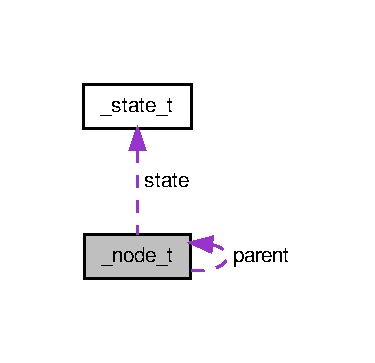
\includegraphics[width=180pt]{d4/d8c/a00035}
\end{center}
\end{figure}
\subsection*{\-Data \-Fields}
\begin{DoxyCompactItemize}
\item 
\hyperlink{a00018_a1c9d0bb39483d4981491e6383b0dbb47_a1c9d0bb39483d4981491e6383b0dbb47}{state\-\_\-t} $\ast$ \hyperlink{a00003_ad180be797ec209ed2712c000b4fd536f_ad180be797ec209ed2712c000b4fd536f}{state}
\item 
\hyperlink{a00020_a9c3f304c1ae0687240efd69b7dc98cd6_a9c3f304c1ae0687240efd69b7dc98cd6}{node\-\_\-t} $\ast$ \hyperlink{a00003_a3d511232fc93632bb149b5932f215a4f_a3d511232fc93632bb149b5932f215a4f}{parent}
\item 
\-G\-S\-List $\ast$ \hyperlink{a00003_a079f3e21ccc72b5e64c1e75be0a9d527_a079f3e21ccc72b5e64c1e75be0a9d527}{children}
\item 
gboolean \hyperlink{a00003_a777bee52ae854bd4b84bddfc8ab97ede_a777bee52ae854bd4b84bddfc8ab97ede}{reaches\-\_\-target}
\item 
double \hyperlink{a00003_a43d03ac887471ca47aaa3e1a99737821_a43d03ac887471ca47aaa3e1a99737821}{distance\-\_\-from\-\_\-parent}
\item 
double \hyperlink{a00003_a8a0362089c7c238279211ee1d3d18f64_a8a0362089c7c238279211ee1d3d18f64}{distance\-\_\-from\-\_\-root}
\item 
\-G\-S\-List $\ast$ \hyperlink{a00003_a5e2ba085667b237c00e4c754c829e9e9_a5e2ba085667b237c00e4c754c829e9e9}{traj\-\_\-from\-\_\-parent}
\item 
\-G\-S\-List $\ast$ \hyperlink{a00003_a3105712d067868a810af6719f032306d_a3105712d067868a810af6719f032306d}{inputs\-\_\-from\-\_\-parent}
\end{DoxyCompactItemize}


\subsection{\-Field \-Documentation}
\hypertarget{a00003_a079f3e21ccc72b5e64c1e75be0a9d527_a079f3e21ccc72b5e64c1e75be0a9d527}{\index{\-\_\-node\-\_\-t@{\-\_\-node\-\_\-t}!children@{children}}
\index{children@{children}!_node_t@{\-\_\-node\-\_\-t}}
\subsubsection[{children}]{\setlength{\rightskip}{0pt plus 5cm}\-G\-S\-List$\ast$ {\bf children}}}\label{d1/d7c/a00003_a079f3e21ccc72b5e64c1e75be0a9d527_a079f3e21ccc72b5e64c1e75be0a9d527}
\hypertarget{a00003_a43d03ac887471ca47aaa3e1a99737821_a43d03ac887471ca47aaa3e1a99737821}{\index{\-\_\-node\-\_\-t@{\-\_\-node\-\_\-t}!distance\-\_\-from\-\_\-parent@{distance\-\_\-from\-\_\-parent}}
\index{distance\-\_\-from\-\_\-parent@{distance\-\_\-from\-\_\-parent}!_node_t@{\-\_\-node\-\_\-t}}
\subsubsection[{distance\-\_\-from\-\_\-parent}]{\setlength{\rightskip}{0pt plus 5cm}double {\bf distance\-\_\-from\-\_\-parent}}}\label{d1/d7c/a00003_a43d03ac887471ca47aaa3e1a99737821_a43d03ac887471ca47aaa3e1a99737821}
\hypertarget{a00003_a8a0362089c7c238279211ee1d3d18f64_a8a0362089c7c238279211ee1d3d18f64}{\index{\-\_\-node\-\_\-t@{\-\_\-node\-\_\-t}!distance\-\_\-from\-\_\-root@{distance\-\_\-from\-\_\-root}}
\index{distance\-\_\-from\-\_\-root@{distance\-\_\-from\-\_\-root}!_node_t@{\-\_\-node\-\_\-t}}
\subsubsection[{distance\-\_\-from\-\_\-root}]{\setlength{\rightskip}{0pt plus 5cm}double {\bf distance\-\_\-from\-\_\-root}}}\label{d1/d7c/a00003_a8a0362089c7c238279211ee1d3d18f64_a8a0362089c7c238279211ee1d3d18f64}
\hypertarget{a00003_a3105712d067868a810af6719f032306d_a3105712d067868a810af6719f032306d}{\index{\-\_\-node\-\_\-t@{\-\_\-node\-\_\-t}!inputs\-\_\-from\-\_\-parent@{inputs\-\_\-from\-\_\-parent}}
\index{inputs\-\_\-from\-\_\-parent@{inputs\-\_\-from\-\_\-parent}!_node_t@{\-\_\-node\-\_\-t}}
\subsubsection[{inputs\-\_\-from\-\_\-parent}]{\setlength{\rightskip}{0pt plus 5cm}\-G\-S\-List$\ast$ {\bf inputs\-\_\-from\-\_\-parent}}}\label{d1/d7c/a00003_a3105712d067868a810af6719f032306d_a3105712d067868a810af6719f032306d}
\hypertarget{a00003_a3d511232fc93632bb149b5932f215a4f_a3d511232fc93632bb149b5932f215a4f}{\index{\-\_\-node\-\_\-t@{\-\_\-node\-\_\-t}!parent@{parent}}
\index{parent@{parent}!_node_t@{\-\_\-node\-\_\-t}}
\subsubsection[{parent}]{\setlength{\rightskip}{0pt plus 5cm}{\bf node\-\_\-t}$\ast$ {\bf parent}}}\label{d1/d7c/a00003_a3d511232fc93632bb149b5932f215a4f_a3d511232fc93632bb149b5932f215a4f}
\hypertarget{a00003_a777bee52ae854bd4b84bddfc8ab97ede_a777bee52ae854bd4b84bddfc8ab97ede}{\index{\-\_\-node\-\_\-t@{\-\_\-node\-\_\-t}!reaches\-\_\-target@{reaches\-\_\-target}}
\index{reaches\-\_\-target@{reaches\-\_\-target}!_node_t@{\-\_\-node\-\_\-t}}
\subsubsection[{reaches\-\_\-target}]{\setlength{\rightskip}{0pt plus 5cm}gboolean {\bf reaches\-\_\-target}}}\label{d1/d7c/a00003_a777bee52ae854bd4b84bddfc8ab97ede_a777bee52ae854bd4b84bddfc8ab97ede}
\hypertarget{a00003_ad180be797ec209ed2712c000b4fd536f_ad180be797ec209ed2712c000b4fd536f}{\index{\-\_\-node\-\_\-t@{\-\_\-node\-\_\-t}!state@{state}}
\index{state@{state}!_node_t@{\-\_\-node\-\_\-t}}
\subsubsection[{state}]{\setlength{\rightskip}{0pt plus 5cm}{\bf state\-\_\-t}$\ast$ {\bf state}}}\label{d1/d7c/a00003_ad180be797ec209ed2712c000b4fd536f_ad180be797ec209ed2712c000b4fd536f}
\hypertarget{a00003_a5e2ba085667b237c00e4c754c829e9e9_a5e2ba085667b237c00e4c754c829e9e9}{\index{\-\_\-node\-\_\-t@{\-\_\-node\-\_\-t}!traj\-\_\-from\-\_\-parent@{traj\-\_\-from\-\_\-parent}}
\index{traj\-\_\-from\-\_\-parent@{traj\-\_\-from\-\_\-parent}!_node_t@{\-\_\-node\-\_\-t}}
\subsubsection[{traj\-\_\-from\-\_\-parent}]{\setlength{\rightskip}{0pt plus 5cm}\-G\-S\-List$\ast$ {\bf traj\-\_\-from\-\_\-parent}}}\label{d1/d7c/a00003_a5e2ba085667b237c00e4c754c829e9e9_a5e2ba085667b237c00e4c754c829e9e9}


\-The documentation for this struct was generated from the following file\-:\begin{DoxyCompactItemize}
\item 
\hyperlink{a00020}{opttree.\-h}\end{DoxyCompactItemize}

\hypertarget{a00004}{\section{\-\_\-optsystem\-\_\-t \-Struct \-Reference}
\label{d0/d0b/a00004}\index{\-\_\-optsystem\-\_\-t@{\-\_\-optsystem\-\_\-t}}
}


{\ttfamily \#include $<$optsystem.\-h$>$}



\-Collaboration diagram for \-\_\-optsystem\-\_\-t\-:\nopagebreak
\begin{figure}[H]
\begin{center}
\leavevmode
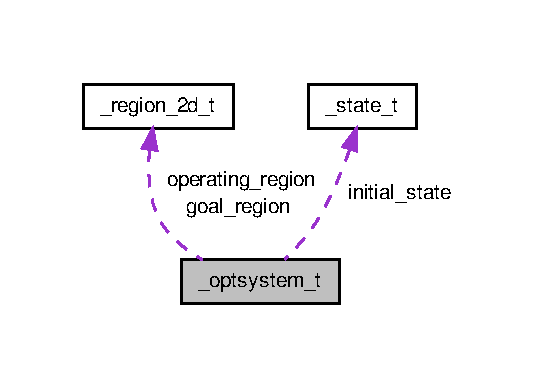
\includegraphics[width=257pt]{de/d8c/a00036}
\end{center}
\end{figure}
\subsection*{\-Data \-Fields}
\begin{DoxyCompactItemize}
\item 
\hyperlink{a00018_a1c9d0bb39483d4981491e6383b0dbb47_a1c9d0bb39483d4981491e6383b0dbb47}{state\-\_\-t} $\ast$ \hyperlink{a00004_ad793fe48f6f4a6d697dc4629f9cb6e91_ad793fe48f6f4a6d697dc4629f9cb6e91}{initial\-\_\-state}
\item 
\hyperlink{a00018_a9136102e25aac8406a94d89f5a95bd1f_a9136102e25aac8406a94d89f5a95bd1f}{region\-\_\-2d\-\_\-t} \hyperlink{a00004_ade92b4bd2437c5d7a474613d0c0c8e95_ade92b4bd2437c5d7a474613d0c0c8e95}{operating\-\_\-region}
\item 
\hyperlink{a00018_a9136102e25aac8406a94d89f5a95bd1f_a9136102e25aac8406a94d89f5a95bd1f}{region\-\_\-2d\-\_\-t} \hyperlink{a00004_a78dce10731005cd5cac846e2eea1a76d_a78dce10731005cd5cac846e2eea1a76d}{goal\-\_\-region}
\item 
\-G\-S\-List $\ast$ \hyperlink{a00004_a5fa7d8df84a6fea47d81dec9cb2c68f2_a5fa7d8df84a6fea47d81dec9cb2c68f2}{obstacle\-\_\-list}
\item 
\-G\-S\-List $\ast$ \hyperlink{a00004_a74c86a6f406deb440600ab0679898043_a74c86a6f406deb440600ab0679898043}{rectangle\-\_\-list}
\end{DoxyCompactItemize}


\subsection{\-Field \-Documentation}
\hypertarget{a00004_a78dce10731005cd5cac846e2eea1a76d_a78dce10731005cd5cac846e2eea1a76d}{\index{\-\_\-optsystem\-\_\-t@{\-\_\-optsystem\-\_\-t}!goal\-\_\-region@{goal\-\_\-region}}
\index{goal\-\_\-region@{goal\-\_\-region}!_optsystem_t@{\-\_\-optsystem\-\_\-t}}
\subsubsection[{goal\-\_\-region}]{\setlength{\rightskip}{0pt plus 5cm}{\bf region\-\_\-2d\-\_\-t} {\bf goal\-\_\-region}}}\label{d0/d0b/a00004_a78dce10731005cd5cac846e2eea1a76d_a78dce10731005cd5cac846e2eea1a76d}
\hypertarget{a00004_ad793fe48f6f4a6d697dc4629f9cb6e91_ad793fe48f6f4a6d697dc4629f9cb6e91}{\index{\-\_\-optsystem\-\_\-t@{\-\_\-optsystem\-\_\-t}!initial\-\_\-state@{initial\-\_\-state}}
\index{initial\-\_\-state@{initial\-\_\-state}!_optsystem_t@{\-\_\-optsystem\-\_\-t}}
\subsubsection[{initial\-\_\-state}]{\setlength{\rightskip}{0pt plus 5cm}{\bf state\-\_\-t}$\ast$ {\bf initial\-\_\-state}}}\label{d0/d0b/a00004_ad793fe48f6f4a6d697dc4629f9cb6e91_ad793fe48f6f4a6d697dc4629f9cb6e91}
\hypertarget{a00004_a5fa7d8df84a6fea47d81dec9cb2c68f2_a5fa7d8df84a6fea47d81dec9cb2c68f2}{\index{\-\_\-optsystem\-\_\-t@{\-\_\-optsystem\-\_\-t}!obstacle\-\_\-list@{obstacle\-\_\-list}}
\index{obstacle\-\_\-list@{obstacle\-\_\-list}!_optsystem_t@{\-\_\-optsystem\-\_\-t}}
\subsubsection[{obstacle\-\_\-list}]{\setlength{\rightskip}{0pt plus 5cm}\-G\-S\-List$\ast$ {\bf obstacle\-\_\-list}}}\label{d0/d0b/a00004_a5fa7d8df84a6fea47d81dec9cb2c68f2_a5fa7d8df84a6fea47d81dec9cb2c68f2}
\hypertarget{a00004_ade92b4bd2437c5d7a474613d0c0c8e95_ade92b4bd2437c5d7a474613d0c0c8e95}{\index{\-\_\-optsystem\-\_\-t@{\-\_\-optsystem\-\_\-t}!operating\-\_\-region@{operating\-\_\-region}}
\index{operating\-\_\-region@{operating\-\_\-region}!_optsystem_t@{\-\_\-optsystem\-\_\-t}}
\subsubsection[{operating\-\_\-region}]{\setlength{\rightskip}{0pt plus 5cm}{\bf region\-\_\-2d\-\_\-t} {\bf operating\-\_\-region}}}\label{d0/d0b/a00004_ade92b4bd2437c5d7a474613d0c0c8e95_ade92b4bd2437c5d7a474613d0c0c8e95}
\hypertarget{a00004_a74c86a6f406deb440600ab0679898043_a74c86a6f406deb440600ab0679898043}{\index{\-\_\-optsystem\-\_\-t@{\-\_\-optsystem\-\_\-t}!rectangle\-\_\-list@{rectangle\-\_\-list}}
\index{rectangle\-\_\-list@{rectangle\-\_\-list}!_optsystem_t@{\-\_\-optsystem\-\_\-t}}
\subsubsection[{rectangle\-\_\-list}]{\setlength{\rightskip}{0pt plus 5cm}\-G\-S\-List$\ast$ {\bf rectangle\-\_\-list}}}\label{d0/d0b/a00004_a74c86a6f406deb440600ab0679898043_a74c86a6f406deb440600ab0679898043}


\-The documentation for this struct was generated from the following file\-:\begin{DoxyCompactItemize}
\item 
\hyperlink{a00018}{optsystem.\-h}\end{DoxyCompactItemize}

\hypertarget{a00005}{\section{\-\_\-opttree\-\_\-t \-Struct \-Reference}
\label{dd/dad/a00005}\index{\-\_\-opttree\-\_\-t@{\-\_\-opttree\-\_\-t}}
}


{\ttfamily \#include $<$opttree.\-h$>$}



\-Collaboration diagram for \-\_\-opttree\-\_\-t\-:\nopagebreak
\begin{figure}[H]
\begin{center}
\leavevmode
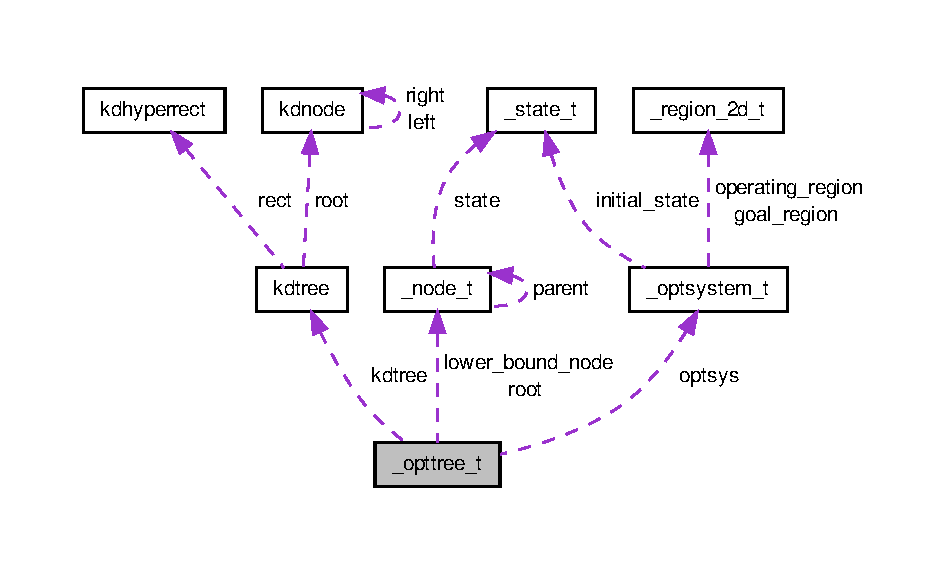
\includegraphics[width=350pt]{d1/dc6/a00037}
\end{center}
\end{figure}
\subsection*{\-Data \-Fields}
\begin{DoxyCompactItemize}
\item 
\hyperlink{a00018_a48d08bbb4534f55ba817743a2b91360c_a48d08bbb4534f55ba817743a2b91360c}{optsystem\-\_\-t} $\ast$ \hyperlink{a00005_ad2d3206cfaefa9f43659e35752c1fdc4_ad2d3206cfaefa9f43659e35752c1fdc4}{optsys}
\item 
\hyperlink{a00020_a3f2e3c0cbfdc70b2db1a09b9aa637a63_a3f2e3c0cbfdc70b2db1a09b9aa637a63}{kdtree\-\_\-t} $\ast$ \hyperlink{a00005_af7ad276e2c2777b487d51d0cfb1e3eba_af7ad276e2c2777b487d51d0cfb1e3eba}{kdtree}
\item 
\hyperlink{a00020_a9c3f304c1ae0687240efd69b7dc98cd6_a9c3f304c1ae0687240efd69b7dc98cd6}{node\-\_\-t} $\ast$ \hyperlink{a00005_a8998e6b3efac0d8d817e301e6522a95e_a8998e6b3efac0d8d817e301e6522a95e}{root}
\item 
\-G\-S\-List $\ast$ \hyperlink{a00005_a36bebfc997ea6923878f45c2ba02bb22_a36bebfc997ea6923878f45c2ba02bb22}{list\-\_\-nodes}
\item 
int \hyperlink{a00005_ae29617de649b665cf0d12c07b31c31d1_ae29617de649b665cf0d12c07b31c31d1}{num\-\_\-nodes}
\item 
gboolean \hyperlink{a00005_a30aad23453eb79f035ecd1fa82acf002_a30aad23453eb79f035ecd1fa82acf002}{run\-\_\-rrtstar}
\item 
double \hyperlink{a00005_a78004c6639270faa551ca8102a2f1a10_a78004c6639270faa551ca8102a2f1a10}{ball\-\_\-radius\-\_\-constant}
\item 
double \hyperlink{a00005_ad248f1aab9c69119356c269d592c4ae1_ad248f1aab9c69119356c269d592c4ae1}{ball\-\_\-radius\-\_\-max}
\item 
double \hyperlink{a00005_aec471f580f2a7649b67117cad9007e4a_aec471f580f2a7649b67117cad9007e4a}{target\-\_\-sample\-\_\-prob\-\_\-before\-\_\-first\-\_\-solution}
\item 
double \hyperlink{a00005_a39416738d060dfec64264e6c7178b8b5_a39416738d060dfec64264e6c7178b8b5}{target\-\_\-sample\-\_\-prob\-\_\-after\-\_\-first\-\_\-solution}
\item 
double \hyperlink{a00005_a8feca8c5101e18b5fdc56936afa01dec_a8feca8c5101e18b5fdc56936afa01dec}{ball\-\_\-radius\-\_\-last}
\item 
double \hyperlink{a00005_a1e2f9a2352c1d9a6cada9544898fceec_a1e2f9a2352c1d9a6cada9544898fceec}{lower\-\_\-bound}
\item 
\hyperlink{a00020_a9c3f304c1ae0687240efd69b7dc98cd6_a9c3f304c1ae0687240efd69b7dc98cd6}{node\-\_\-t} $\ast$ \hyperlink{a00005_ad3729166dd83f52a5e03e65a83eef6e7_ad3729166dd83f52a5e03e65a83eef6e7}{lower\-\_\-bound\-\_\-node}
\end{DoxyCompactItemize}


\subsection{\-Field \-Documentation}
\hypertarget{a00005_a78004c6639270faa551ca8102a2f1a10_a78004c6639270faa551ca8102a2f1a10}{\index{\-\_\-opttree\-\_\-t@{\-\_\-opttree\-\_\-t}!ball\-\_\-radius\-\_\-constant@{ball\-\_\-radius\-\_\-constant}}
\index{ball\-\_\-radius\-\_\-constant@{ball\-\_\-radius\-\_\-constant}!_opttree_t@{\-\_\-opttree\-\_\-t}}
\subsubsection[{ball\-\_\-radius\-\_\-constant}]{\setlength{\rightskip}{0pt plus 5cm}double {\bf ball\-\_\-radius\-\_\-constant}}}\label{dd/dad/a00005_a78004c6639270faa551ca8102a2f1a10_a78004c6639270faa551ca8102a2f1a10}
\hypertarget{a00005_a8feca8c5101e18b5fdc56936afa01dec_a8feca8c5101e18b5fdc56936afa01dec}{\index{\-\_\-opttree\-\_\-t@{\-\_\-opttree\-\_\-t}!ball\-\_\-radius\-\_\-last@{ball\-\_\-radius\-\_\-last}}
\index{ball\-\_\-radius\-\_\-last@{ball\-\_\-radius\-\_\-last}!_opttree_t@{\-\_\-opttree\-\_\-t}}
\subsubsection[{ball\-\_\-radius\-\_\-last}]{\setlength{\rightskip}{0pt plus 5cm}double {\bf ball\-\_\-radius\-\_\-last}}}\label{dd/dad/a00005_a8feca8c5101e18b5fdc56936afa01dec_a8feca8c5101e18b5fdc56936afa01dec}
\hypertarget{a00005_ad248f1aab9c69119356c269d592c4ae1_ad248f1aab9c69119356c269d592c4ae1}{\index{\-\_\-opttree\-\_\-t@{\-\_\-opttree\-\_\-t}!ball\-\_\-radius\-\_\-max@{ball\-\_\-radius\-\_\-max}}
\index{ball\-\_\-radius\-\_\-max@{ball\-\_\-radius\-\_\-max}!_opttree_t@{\-\_\-opttree\-\_\-t}}
\subsubsection[{ball\-\_\-radius\-\_\-max}]{\setlength{\rightskip}{0pt plus 5cm}double {\bf ball\-\_\-radius\-\_\-max}}}\label{dd/dad/a00005_ad248f1aab9c69119356c269d592c4ae1_ad248f1aab9c69119356c269d592c4ae1}
\hypertarget{a00005_af7ad276e2c2777b487d51d0cfb1e3eba_af7ad276e2c2777b487d51d0cfb1e3eba}{\index{\-\_\-opttree\-\_\-t@{\-\_\-opttree\-\_\-t}!kdtree@{kdtree}}
\index{kdtree@{kdtree}!_opttree_t@{\-\_\-opttree\-\_\-t}}
\subsubsection[{kdtree}]{\setlength{\rightskip}{0pt plus 5cm}{\bf kdtree\-\_\-t}$\ast$ {\bf kdtree}}}\label{dd/dad/a00005_af7ad276e2c2777b487d51d0cfb1e3eba_af7ad276e2c2777b487d51d0cfb1e3eba}
\hypertarget{a00005_a36bebfc997ea6923878f45c2ba02bb22_a36bebfc997ea6923878f45c2ba02bb22}{\index{\-\_\-opttree\-\_\-t@{\-\_\-opttree\-\_\-t}!list\-\_\-nodes@{list\-\_\-nodes}}
\index{list\-\_\-nodes@{list\-\_\-nodes}!_opttree_t@{\-\_\-opttree\-\_\-t}}
\subsubsection[{list\-\_\-nodes}]{\setlength{\rightskip}{0pt plus 5cm}\-G\-S\-List$\ast$ {\bf list\-\_\-nodes}}}\label{dd/dad/a00005_a36bebfc997ea6923878f45c2ba02bb22_a36bebfc997ea6923878f45c2ba02bb22}
\hypertarget{a00005_a1e2f9a2352c1d9a6cada9544898fceec_a1e2f9a2352c1d9a6cada9544898fceec}{\index{\-\_\-opttree\-\_\-t@{\-\_\-opttree\-\_\-t}!lower\-\_\-bound@{lower\-\_\-bound}}
\index{lower\-\_\-bound@{lower\-\_\-bound}!_opttree_t@{\-\_\-opttree\-\_\-t}}
\subsubsection[{lower\-\_\-bound}]{\setlength{\rightskip}{0pt plus 5cm}double {\bf lower\-\_\-bound}}}\label{dd/dad/a00005_a1e2f9a2352c1d9a6cada9544898fceec_a1e2f9a2352c1d9a6cada9544898fceec}
\hypertarget{a00005_ad3729166dd83f52a5e03e65a83eef6e7_ad3729166dd83f52a5e03e65a83eef6e7}{\index{\-\_\-opttree\-\_\-t@{\-\_\-opttree\-\_\-t}!lower\-\_\-bound\-\_\-node@{lower\-\_\-bound\-\_\-node}}
\index{lower\-\_\-bound\-\_\-node@{lower\-\_\-bound\-\_\-node}!_opttree_t@{\-\_\-opttree\-\_\-t}}
\subsubsection[{lower\-\_\-bound\-\_\-node}]{\setlength{\rightskip}{0pt plus 5cm}{\bf node\-\_\-t}$\ast$ {\bf lower\-\_\-bound\-\_\-node}}}\label{dd/dad/a00005_ad3729166dd83f52a5e03e65a83eef6e7_ad3729166dd83f52a5e03e65a83eef6e7}
\hypertarget{a00005_ae29617de649b665cf0d12c07b31c31d1_ae29617de649b665cf0d12c07b31c31d1}{\index{\-\_\-opttree\-\_\-t@{\-\_\-opttree\-\_\-t}!num\-\_\-nodes@{num\-\_\-nodes}}
\index{num\-\_\-nodes@{num\-\_\-nodes}!_opttree_t@{\-\_\-opttree\-\_\-t}}
\subsubsection[{num\-\_\-nodes}]{\setlength{\rightskip}{0pt plus 5cm}int {\bf num\-\_\-nodes}}}\label{dd/dad/a00005_ae29617de649b665cf0d12c07b31c31d1_ae29617de649b665cf0d12c07b31c31d1}
\hypertarget{a00005_ad2d3206cfaefa9f43659e35752c1fdc4_ad2d3206cfaefa9f43659e35752c1fdc4}{\index{\-\_\-opttree\-\_\-t@{\-\_\-opttree\-\_\-t}!optsys@{optsys}}
\index{optsys@{optsys}!_opttree_t@{\-\_\-opttree\-\_\-t}}
\subsubsection[{optsys}]{\setlength{\rightskip}{0pt plus 5cm}{\bf optsystem\-\_\-t}$\ast$ {\bf optsys}}}\label{dd/dad/a00005_ad2d3206cfaefa9f43659e35752c1fdc4_ad2d3206cfaefa9f43659e35752c1fdc4}
\hypertarget{a00005_a8998e6b3efac0d8d817e301e6522a95e_a8998e6b3efac0d8d817e301e6522a95e}{\index{\-\_\-opttree\-\_\-t@{\-\_\-opttree\-\_\-t}!root@{root}}
\index{root@{root}!_opttree_t@{\-\_\-opttree\-\_\-t}}
\subsubsection[{root}]{\setlength{\rightskip}{0pt plus 5cm}{\bf node\-\_\-t}$\ast$ {\bf root}}}\label{dd/dad/a00005_a8998e6b3efac0d8d817e301e6522a95e_a8998e6b3efac0d8d817e301e6522a95e}
\hypertarget{a00005_a30aad23453eb79f035ecd1fa82acf002_a30aad23453eb79f035ecd1fa82acf002}{\index{\-\_\-opttree\-\_\-t@{\-\_\-opttree\-\_\-t}!run\-\_\-rrtstar@{run\-\_\-rrtstar}}
\index{run\-\_\-rrtstar@{run\-\_\-rrtstar}!_opttree_t@{\-\_\-opttree\-\_\-t}}
\subsubsection[{run\-\_\-rrtstar}]{\setlength{\rightskip}{0pt plus 5cm}gboolean {\bf run\-\_\-rrtstar}}}\label{dd/dad/a00005_a30aad23453eb79f035ecd1fa82acf002_a30aad23453eb79f035ecd1fa82acf002}
\hypertarget{a00005_a39416738d060dfec64264e6c7178b8b5_a39416738d060dfec64264e6c7178b8b5}{\index{\-\_\-opttree\-\_\-t@{\-\_\-opttree\-\_\-t}!target\-\_\-sample\-\_\-prob\-\_\-after\-\_\-first\-\_\-solution@{target\-\_\-sample\-\_\-prob\-\_\-after\-\_\-first\-\_\-solution}}
\index{target\-\_\-sample\-\_\-prob\-\_\-after\-\_\-first\-\_\-solution@{target\-\_\-sample\-\_\-prob\-\_\-after\-\_\-first\-\_\-solution}!_opttree_t@{\-\_\-opttree\-\_\-t}}
\subsubsection[{target\-\_\-sample\-\_\-prob\-\_\-after\-\_\-first\-\_\-solution}]{\setlength{\rightskip}{0pt plus 5cm}double {\bf target\-\_\-sample\-\_\-prob\-\_\-after\-\_\-first\-\_\-solution}}}\label{dd/dad/a00005_a39416738d060dfec64264e6c7178b8b5_a39416738d060dfec64264e6c7178b8b5}
\hypertarget{a00005_aec471f580f2a7649b67117cad9007e4a_aec471f580f2a7649b67117cad9007e4a}{\index{\-\_\-opttree\-\_\-t@{\-\_\-opttree\-\_\-t}!target\-\_\-sample\-\_\-prob\-\_\-before\-\_\-first\-\_\-solution@{target\-\_\-sample\-\_\-prob\-\_\-before\-\_\-first\-\_\-solution}}
\index{target\-\_\-sample\-\_\-prob\-\_\-before\-\_\-first\-\_\-solution@{target\-\_\-sample\-\_\-prob\-\_\-before\-\_\-first\-\_\-solution}!_opttree_t@{\-\_\-opttree\-\_\-t}}
\subsubsection[{target\-\_\-sample\-\_\-prob\-\_\-before\-\_\-first\-\_\-solution}]{\setlength{\rightskip}{0pt plus 5cm}double {\bf target\-\_\-sample\-\_\-prob\-\_\-before\-\_\-first\-\_\-solution}}}\label{dd/dad/a00005_aec471f580f2a7649b67117cad9007e4a_aec471f580f2a7649b67117cad9007e4a}


\-The documentation for this struct was generated from the following file\-:\begin{DoxyCompactItemize}
\item 
\hyperlink{a00020}{opttree.\-h}\end{DoxyCompactItemize}

\hypertarget{a00006}{\section{\-\_\-region\-\_\-2d\-\_\-t \-Struct \-Reference}
\label{de/d21/a00006}\index{\-\_\-region\-\_\-2d\-\_\-t@{\-\_\-region\-\_\-2d\-\_\-t}}
}


{\ttfamily \#include $<$optsystem.\-h$>$}

\subsection*{\-Data \-Fields}
\begin{DoxyCompactItemize}
\item 
double \hyperlink{a00006_a00e863db26745564c8e171606f0900e2_a00e863db26745564c8e171606f0900e2}{center} \mbox{[}2\mbox{]}
\item 
double \hyperlink{a00006_ad1af25ff64d4bcccf1c67fb516a10b13_ad1af25ff64d4bcccf1c67fb516a10b13}{size} \mbox{[}2\mbox{]}
\end{DoxyCompactItemize}


\subsection{\-Field \-Documentation}
\hypertarget{a00006_a00e863db26745564c8e171606f0900e2_a00e863db26745564c8e171606f0900e2}{\index{\-\_\-region\-\_\-2d\-\_\-t@{\-\_\-region\-\_\-2d\-\_\-t}!center@{center}}
\index{center@{center}!_region_2d_t@{\-\_\-region\-\_\-2d\-\_\-t}}
\subsubsection[{center}]{\setlength{\rightskip}{0pt plus 5cm}double {\bf center}\mbox{[}2\mbox{]}}}\label{de/d21/a00006_a00e863db26745564c8e171606f0900e2_a00e863db26745564c8e171606f0900e2}
\hypertarget{a00006_ad1af25ff64d4bcccf1c67fb516a10b13_ad1af25ff64d4bcccf1c67fb516a10b13}{\index{\-\_\-region\-\_\-2d\-\_\-t@{\-\_\-region\-\_\-2d\-\_\-t}!size@{size}}
\index{size@{size}!_region_2d_t@{\-\_\-region\-\_\-2d\-\_\-t}}
\subsubsection[{size}]{\setlength{\rightskip}{0pt plus 5cm}double {\bf size}\mbox{[}2\mbox{]}}}\label{de/d21/a00006_ad1af25ff64d4bcccf1c67fb516a10b13_ad1af25ff64d4bcccf1c67fb516a10b13}


\-The documentation for this struct was generated from the following file\-:\begin{DoxyCompactItemize}
\item 
\hyperlink{a00018}{optsystem.\-h}\end{DoxyCompactItemize}

\hypertarget{a00007}{\section{\-\_\-state\-\_\-t \-Struct \-Reference}
\label{de/d5e/a00007}\index{\-\_\-state\-\_\-t@{\-\_\-state\-\_\-t}}
}


{\ttfamily \#include $<$optsystem.\-h$>$}

\subsection*{\-Data \-Fields}
\begin{DoxyCompactItemize}
\item 
double \hyperlink{a00007_ab1632e02642e8b20f337b10daa3cf5c2_ab1632e02642e8b20f337b10daa3cf5c2}{x} \mbox{[}\hyperlink{a00018_a6e67a587012cd0570839daca590cf822_a6e67a587012cd0570839daca590cf822}{\-N\-U\-M\-\_\-\-S\-T\-A\-T\-E\-S}\mbox{]}
\end{DoxyCompactItemize}


\subsection{\-Field \-Documentation}
\hypertarget{a00007_ab1632e02642e8b20f337b10daa3cf5c2_ab1632e02642e8b20f337b10daa3cf5c2}{\index{\-\_\-state\-\_\-t@{\-\_\-state\-\_\-t}!x@{x}}
\index{x@{x}!_state_t@{\-\_\-state\-\_\-t}}
\subsubsection[{x}]{\setlength{\rightskip}{0pt plus 5cm}double {\bf x}\mbox{[}{\bf \-N\-U\-M\-\_\-\-S\-T\-A\-T\-E\-S}\mbox{]}}}\label{de/d5e/a00007_ab1632e02642e8b20f337b10daa3cf5c2_ab1632e02642e8b20f337b10daa3cf5c2}


\-The documentation for this struct was generated from the following file\-:\begin{DoxyCompactItemize}
\item 
\hyperlink{a00018}{optsystem.\-h}\end{DoxyCompactItemize}

\hypertarget{a00008}{\section{kdhyperrect \-Struct \-Reference}
\label{d4/dee/a00008}\index{kdhyperrect@{kdhyperrect}}
}
\subsection*{\-Data \-Fields}
\begin{DoxyCompactItemize}
\item 
int \hyperlink{a00008_a70b5e28b5bc3d1b63a7435c5fe50b837_a70b5e28b5bc3d1b63a7435c5fe50b837}{dim}
\item 
double $\ast$ \hyperlink{a00008_a84ea468000e399560bbee8281490337d_a84ea468000e399560bbee8281490337d}{min}
\item 
double $\ast$ \hyperlink{a00008_a1a9be85667cb2f50d8abcfcb4edb17c7_a1a9be85667cb2f50d8abcfcb4edb17c7}{max}
\end{DoxyCompactItemize}


\subsection{\-Field \-Documentation}
\hypertarget{a00008_a70b5e28b5bc3d1b63a7435c5fe50b837_a70b5e28b5bc3d1b63a7435c5fe50b837}{\index{kdhyperrect@{kdhyperrect}!dim@{dim}}
\index{dim@{dim}!kdhyperrect@{kdhyperrect}}
\subsubsection[{dim}]{\setlength{\rightskip}{0pt plus 5cm}int {\bf dim}}}\label{d4/dee/a00008_a70b5e28b5bc3d1b63a7435c5fe50b837_a70b5e28b5bc3d1b63a7435c5fe50b837}
\hypertarget{a00008_a1a9be85667cb2f50d8abcfcb4edb17c7_a1a9be85667cb2f50d8abcfcb4edb17c7}{\index{kdhyperrect@{kdhyperrect}!max@{max}}
\index{max@{max}!kdhyperrect@{kdhyperrect}}
\subsubsection[{max}]{\setlength{\rightskip}{0pt plus 5cm}double $\ast$ {\bf max}}}\label{d4/dee/a00008_a1a9be85667cb2f50d8abcfcb4edb17c7_a1a9be85667cb2f50d8abcfcb4edb17c7}
\hypertarget{a00008_a84ea468000e399560bbee8281490337d_a84ea468000e399560bbee8281490337d}{\index{kdhyperrect@{kdhyperrect}!min@{min}}
\index{min@{min}!kdhyperrect@{kdhyperrect}}
\subsubsection[{min}]{\setlength{\rightskip}{0pt plus 5cm}double$\ast$ {\bf min}}}\label{d4/dee/a00008_a84ea468000e399560bbee8281490337d_a84ea468000e399560bbee8281490337d}


\-The documentation for this struct was generated from the following file\-:\begin{DoxyCompactItemize}
\item 
\hyperlink{a00013}{kdtree.\-c}\end{DoxyCompactItemize}

\hypertarget{a00009}{\section{kdnode \-Struct \-Reference}
\label{da/da0/a00009}\index{kdnode@{kdnode}}
}


\-Collaboration diagram for kdnode\-:\nopagebreak
\begin{figure}[H]
\begin{center}
\leavevmode
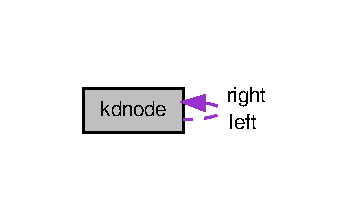
\includegraphics[width=168pt]{d8/d41/a00038}
\end{center}
\end{figure}
\subsection*{\-Data \-Fields}
\begin{DoxyCompactItemize}
\item 
double $\ast$ \hyperlink{a00009_a1a6076b5177bd7af0d55bc0e8c21fde3_a1a6076b5177bd7af0d55bc0e8c21fde3}{pos}
\item 
int \hyperlink{a00009_a851cf68c8f607573c1a5e987784c83f6_a851cf68c8f607573c1a5e987784c83f6}{dir}
\item 
void $\ast$ \hyperlink{a00009_a735984d41155bc1032e09bece8f8d66d_a735984d41155bc1032e09bece8f8d66d}{data}
\item 
struct \hyperlink{a00009}{kdnode} $\ast$ \hyperlink{a00009_a77fe629b496db8e95613fa6520af4371_a77fe629b496db8e95613fa6520af4371}{left}
\item 
struct \hyperlink{a00009}{kdnode} $\ast$ \hyperlink{a00009_ad73ae7970017da6a7f7fafc2e889bb51_ad73ae7970017da6a7f7fafc2e889bb51}{right}
\end{DoxyCompactItemize}


\subsection{\-Field \-Documentation}
\hypertarget{a00009_a735984d41155bc1032e09bece8f8d66d_a735984d41155bc1032e09bece8f8d66d}{\index{kdnode@{kdnode}!data@{data}}
\index{data@{data}!kdnode@{kdnode}}
\subsubsection[{data}]{\setlength{\rightskip}{0pt plus 5cm}void$\ast$ {\bf data}}}\label{da/da0/a00009_a735984d41155bc1032e09bece8f8d66d_a735984d41155bc1032e09bece8f8d66d}
\hypertarget{a00009_a851cf68c8f607573c1a5e987784c83f6_a851cf68c8f607573c1a5e987784c83f6}{\index{kdnode@{kdnode}!dir@{dir}}
\index{dir@{dir}!kdnode@{kdnode}}
\subsubsection[{dir}]{\setlength{\rightskip}{0pt plus 5cm}int {\bf dir}}}\label{da/da0/a00009_a851cf68c8f607573c1a5e987784c83f6_a851cf68c8f607573c1a5e987784c83f6}
\hypertarget{a00009_a77fe629b496db8e95613fa6520af4371_a77fe629b496db8e95613fa6520af4371}{\index{kdnode@{kdnode}!left@{left}}
\index{left@{left}!kdnode@{kdnode}}
\subsubsection[{left}]{\setlength{\rightskip}{0pt plus 5cm}struct {\bf kdnode}$\ast$ {\bf left}}}\label{da/da0/a00009_a77fe629b496db8e95613fa6520af4371_a77fe629b496db8e95613fa6520af4371}
\hypertarget{a00009_a1a6076b5177bd7af0d55bc0e8c21fde3_a1a6076b5177bd7af0d55bc0e8c21fde3}{\index{kdnode@{kdnode}!pos@{pos}}
\index{pos@{pos}!kdnode@{kdnode}}
\subsubsection[{pos}]{\setlength{\rightskip}{0pt plus 5cm}double$\ast$ {\bf pos}}}\label{da/da0/a00009_a1a6076b5177bd7af0d55bc0e8c21fde3_a1a6076b5177bd7af0d55bc0e8c21fde3}
\hypertarget{a00009_ad73ae7970017da6a7f7fafc2e889bb51_ad73ae7970017da6a7f7fafc2e889bb51}{\index{kdnode@{kdnode}!right@{right}}
\index{right@{right}!kdnode@{kdnode}}
\subsubsection[{right}]{\setlength{\rightskip}{0pt plus 5cm}struct {\bf kdnode} $\ast$ {\bf right}}}\label{da/da0/a00009_ad73ae7970017da6a7f7fafc2e889bb51_ad73ae7970017da6a7f7fafc2e889bb51}


\-The documentation for this struct was generated from the following file\-:\begin{DoxyCompactItemize}
\item 
\hyperlink{a00013}{kdtree.\-c}\end{DoxyCompactItemize}

\hypertarget{a00010}{\section{kdres \-Struct \-Reference}
\label{d7/dec/a00010}\index{kdres@{kdres}}
}


\-Collaboration diagram for kdres\-:\nopagebreak
\begin{figure}[H]
\begin{center}
\leavevmode
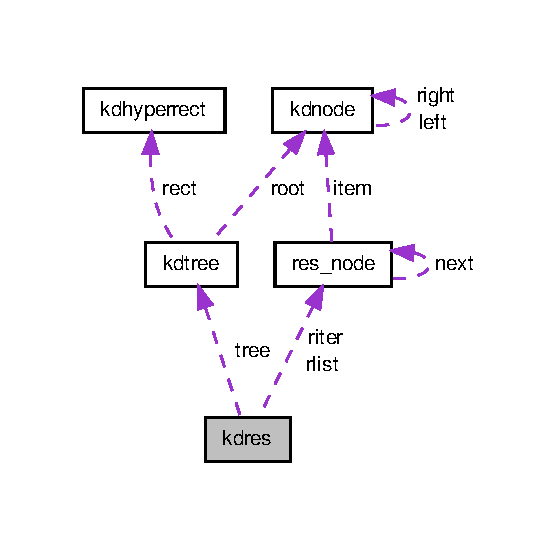
\includegraphics[width=268pt]{d3/de7/a00039}
\end{center}
\end{figure}
\subsection*{\-Data \-Fields}
\begin{DoxyCompactItemize}
\item 
struct \hyperlink{a00011}{kdtree} $\ast$ \hyperlink{a00010_ae75a12d07763fe14039f5123e1e3d377_ae75a12d07763fe14039f5123e1e3d377}{tree}
\item 
struct \hyperlink{a00012}{res\-\_\-node} $\ast$ \hyperlink{a00010_a1424ef73f7eb289a18a4ce40ac38dedb_a1424ef73f7eb289a18a4ce40ac38dedb}{rlist}
\item 
struct \hyperlink{a00012}{res\-\_\-node} $\ast$ \hyperlink{a00010_a10ec50599e37f9fcb520b8fc6d44728b_a10ec50599e37f9fcb520b8fc6d44728b}{riter}
\item 
int \hyperlink{a00010_a439227feff9d7f55384e8780cfc2eb82_a439227feff9d7f55384e8780cfc2eb82}{size}
\end{DoxyCompactItemize}


\subsection{\-Field \-Documentation}
\hypertarget{a00010_a10ec50599e37f9fcb520b8fc6d44728b_a10ec50599e37f9fcb520b8fc6d44728b}{\index{kdres@{kdres}!riter@{riter}}
\index{riter@{riter}!kdres@{kdres}}
\subsubsection[{riter}]{\setlength{\rightskip}{0pt plus 5cm}struct {\bf res\-\_\-node} $\ast$ {\bf riter}}}\label{d7/dec/a00010_a10ec50599e37f9fcb520b8fc6d44728b_a10ec50599e37f9fcb520b8fc6d44728b}
\hypertarget{a00010_a1424ef73f7eb289a18a4ce40ac38dedb_a1424ef73f7eb289a18a4ce40ac38dedb}{\index{kdres@{kdres}!rlist@{rlist}}
\index{rlist@{rlist}!kdres@{kdres}}
\subsubsection[{rlist}]{\setlength{\rightskip}{0pt plus 5cm}struct {\bf res\-\_\-node}$\ast$ {\bf rlist}}}\label{d7/dec/a00010_a1424ef73f7eb289a18a4ce40ac38dedb_a1424ef73f7eb289a18a4ce40ac38dedb}
\hypertarget{a00010_a439227feff9d7f55384e8780cfc2eb82_a439227feff9d7f55384e8780cfc2eb82}{\index{kdres@{kdres}!size@{size}}
\index{size@{size}!kdres@{kdres}}
\subsubsection[{size}]{\setlength{\rightskip}{0pt plus 5cm}int {\bf size}}}\label{d7/dec/a00010_a439227feff9d7f55384e8780cfc2eb82_a439227feff9d7f55384e8780cfc2eb82}
\hypertarget{a00010_ae75a12d07763fe14039f5123e1e3d377_ae75a12d07763fe14039f5123e1e3d377}{\index{kdres@{kdres}!tree@{tree}}
\index{tree@{tree}!kdres@{kdres}}
\subsubsection[{tree}]{\setlength{\rightskip}{0pt plus 5cm}struct {\bf kdtree}$\ast$ {\bf tree}}}\label{d7/dec/a00010_ae75a12d07763fe14039f5123e1e3d377_ae75a12d07763fe14039f5123e1e3d377}


\-The documentation for this struct was generated from the following file\-:\begin{DoxyCompactItemize}
\item 
\hyperlink{a00013}{kdtree.\-c}\end{DoxyCompactItemize}

\hypertarget{a00011}{\section{kdtree \-Struct \-Reference}
\label{da/d45/a00011}\index{kdtree@{kdtree}}
}


\-Collaboration diagram for kdtree\-:\nopagebreak
\begin{figure}[H]
\begin{center}
\leavevmode
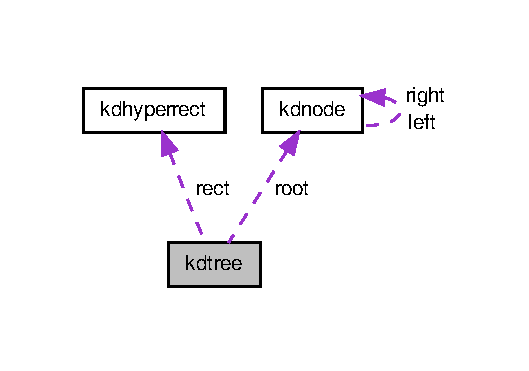
\includegraphics[width=254pt]{db/d3a/a00040}
\end{center}
\end{figure}
\subsection*{\-Data \-Fields}
\begin{DoxyCompactItemize}
\item 
int \hyperlink{a00011_a70b5e28b5bc3d1b63a7435c5fe50b837_a70b5e28b5bc3d1b63a7435c5fe50b837}{dim}
\item 
struct \hyperlink{a00009}{kdnode} $\ast$ \hyperlink{a00011_a75f7244d061840423e44a33990f08d07_a75f7244d061840423e44a33990f08d07}{root}
\item 
struct \hyperlink{a00008}{kdhyperrect} $\ast$ \hyperlink{a00011_aa40b9a36013f3e2014bd44fb27909ca2_aa40b9a36013f3e2014bd44fb27909ca2}{rect}
\item 
void($\ast$ \hyperlink{a00011_a7d06069e4fb5ffe40d5db88c0081f3ac_a7d06069e4fb5ffe40d5db88c0081f3ac}{destr} )(void $\ast$)
\end{DoxyCompactItemize}


\subsection{\-Field \-Documentation}
\hypertarget{a00011_a7d06069e4fb5ffe40d5db88c0081f3ac_a7d06069e4fb5ffe40d5db88c0081f3ac}{\index{kdtree@{kdtree}!destr@{destr}}
\index{destr@{destr}!kdtree@{kdtree}}
\subsubsection[{destr}]{\setlength{\rightskip}{0pt plus 5cm}void($\ast$ {\bf destr})(void $\ast$)}}\label{da/d45/a00011_a7d06069e4fb5ffe40d5db88c0081f3ac_a7d06069e4fb5ffe40d5db88c0081f3ac}
\hypertarget{a00011_a70b5e28b5bc3d1b63a7435c5fe50b837_a70b5e28b5bc3d1b63a7435c5fe50b837}{\index{kdtree@{kdtree}!dim@{dim}}
\index{dim@{dim}!kdtree@{kdtree}}
\subsubsection[{dim}]{\setlength{\rightskip}{0pt plus 5cm}int {\bf dim}}}\label{da/d45/a00011_a70b5e28b5bc3d1b63a7435c5fe50b837_a70b5e28b5bc3d1b63a7435c5fe50b837}
\hypertarget{a00011_aa40b9a36013f3e2014bd44fb27909ca2_aa40b9a36013f3e2014bd44fb27909ca2}{\index{kdtree@{kdtree}!rect@{rect}}
\index{rect@{rect}!kdtree@{kdtree}}
\subsubsection[{rect}]{\setlength{\rightskip}{0pt plus 5cm}struct {\bf kdhyperrect}$\ast$ {\bf rect}}}\label{da/d45/a00011_aa40b9a36013f3e2014bd44fb27909ca2_aa40b9a36013f3e2014bd44fb27909ca2}
\hypertarget{a00011_a75f7244d061840423e44a33990f08d07_a75f7244d061840423e44a33990f08d07}{\index{kdtree@{kdtree}!root@{root}}
\index{root@{root}!kdtree@{kdtree}}
\subsubsection[{root}]{\setlength{\rightskip}{0pt plus 5cm}struct {\bf kdnode}$\ast$ {\bf root}}}\label{da/d45/a00011_a75f7244d061840423e44a33990f08d07_a75f7244d061840423e44a33990f08d07}


\-The documentation for this struct was generated from the following file\-:\begin{DoxyCompactItemize}
\item 
\hyperlink{a00013}{kdtree.\-c}\end{DoxyCompactItemize}

\hypertarget{a00012}{\section{res\-\_\-node \-Struct \-Reference}
\label{df/d86/a00012}\index{res\-\_\-node@{res\-\_\-node}}
}


\-Collaboration diagram for res\-\_\-node\-:
\nopagebreak
\begin{figure}[H]
\begin{center}
\leavevmode
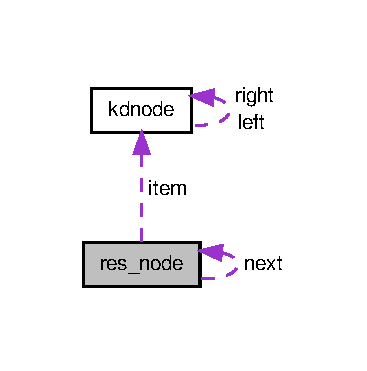
\includegraphics[width=176pt]{dd/d32/a00041}
\end{center}
\end{figure}
\subsection*{\-Data \-Fields}
\begin{DoxyCompactItemize}
\item 
struct \hyperlink{a00009}{kdnode} $\ast$ \hyperlink{a00012_a9839da196515787759722e34b14a2d3f_a9839da196515787759722e34b14a2d3f}{item}
\item 
double \hyperlink{a00012_ab5db408f198264d49229dc7119b5a259_ab5db408f198264d49229dc7119b5a259}{dist\-\_\-sq}
\item 
struct \hyperlink{a00012}{res\-\_\-node} $\ast$ \hyperlink{a00012_a4a322132f093f66e895e0b5f5ee1bfea_a4a322132f093f66e895e0b5f5ee1bfea}{next}
\end{DoxyCompactItemize}


\subsection{\-Field \-Documentation}
\hypertarget{a00012_ab5db408f198264d49229dc7119b5a259_ab5db408f198264d49229dc7119b5a259}{\index{res\-\_\-node@{res\-\_\-node}!dist\-\_\-sq@{dist\-\_\-sq}}
\index{dist\-\_\-sq@{dist\-\_\-sq}!res_node@{res\-\_\-node}}
\subsubsection[{dist\-\_\-sq}]{\setlength{\rightskip}{0pt plus 5cm}double {\bf dist\-\_\-sq}}}\label{df/d86/a00012_ab5db408f198264d49229dc7119b5a259_ab5db408f198264d49229dc7119b5a259}
\hypertarget{a00012_a9839da196515787759722e34b14a2d3f_a9839da196515787759722e34b14a2d3f}{\index{res\-\_\-node@{res\-\_\-node}!item@{item}}
\index{item@{item}!res_node@{res\-\_\-node}}
\subsubsection[{item}]{\setlength{\rightskip}{0pt plus 5cm}struct {\bf kdnode}$\ast$ {\bf item}}}\label{df/d86/a00012_a9839da196515787759722e34b14a2d3f_a9839da196515787759722e34b14a2d3f}
\hypertarget{a00012_a4a322132f093f66e895e0b5f5ee1bfea_a4a322132f093f66e895e0b5f5ee1bfea}{\index{res\-\_\-node@{res\-\_\-node}!next@{next}}
\index{next@{next}!res_node@{res\-\_\-node}}
\subsubsection[{next}]{\setlength{\rightskip}{0pt plus 5cm}struct {\bf res\-\_\-node}$\ast$ {\bf next}}}\label{df/d86/a00012_a4a322132f093f66e895e0b5f5ee1bfea_a4a322132f093f66e895e0b5f5ee1bfea}


\-The documentation for this struct was generated from the following file\-:\begin{DoxyCompactItemize}
\item 
\hyperlink{a00013}{kdtree.\-c}\end{DoxyCompactItemize}

\chapter{\-File \-Documentation}
\hypertarget{a00013}{\section{kdtree.\-c \-File \-Reference}
\label{d7/dd4/a00013}\index{kdtree.\-c@{kdtree.\-c}}
}
{\ttfamily \#include $<$stdio.\-h$>$}\*
{\ttfamily \#include $<$stdlib.\-h$>$}\*
{\ttfamily \#include $<$string.\-h$>$}\*
{\ttfamily \#include $<$math.\-h$>$}\*
{\ttfamily \#include \char`\"{}kdtree.\-h\char`\"{}}\*
\-Include dependency graph for kdtree.\-c\-:\nopagebreak
\begin{figure}[H]
\begin{center}
\leavevmode
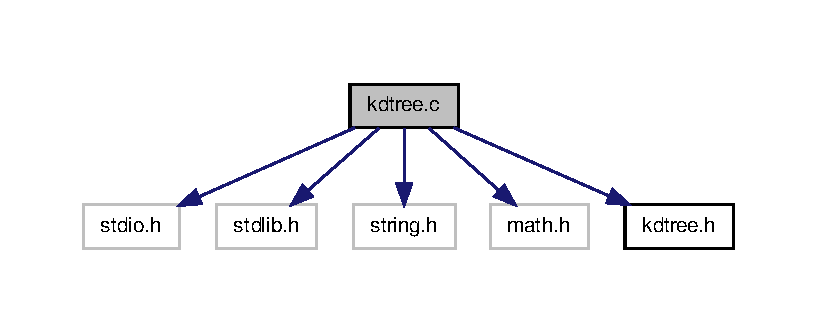
\includegraphics[width=350pt]{d3/d52/a00023}
\end{center}
\end{figure}
\subsection*{\-Data \-Structures}
\begin{DoxyCompactItemize}
\item 
struct \hyperlink{a00008}{kdhyperrect}
\item 
struct \hyperlink{a00009}{kdnode}
\item 
struct \hyperlink{a00012}{res\-\_\-node}
\item 
struct \hyperlink{a00011}{kdtree}
\item 
struct \hyperlink{a00010}{kdres}
\end{DoxyCompactItemize}
\subsection*{\-Defines}
\begin{DoxyCompactItemize}
\item 
\#define \hyperlink{a00013_ac3644f84794a8bfdacf39c4b2c2495fc_ac3644f84794a8bfdacf39c4b2c2495fc}{\-S\-Q}(x)~((x) $\ast$ (x))
\item 
\#define \hyperlink{a00013_aeb41ddbd68313adcb5129add2c4428d0_aeb41ddbd68313adcb5129add2c4428d0}{alloc\-\_\-resnode}()~malloc(sizeof(struct \hyperlink{a00012}{res\-\_\-node}))
\item 
\#define \hyperlink{a00013_aa809c41131ed043aab5ea2f7806fa458_aa809c41131ed043aab5ea2f7806fa458}{free\-\_\-resnode}(n)~free(n)
\end{DoxyCompactItemize}
\subsection*{\-Functions}
\begin{DoxyCompactItemize}
\item 
struct \hyperlink{a00011}{kdtree} $\ast$ \hyperlink{a00013_a0267f17ca84a70322af662b16a625c16_a0267f17ca84a70322af662b16a625c16}{kd\-\_\-create} (int k)
\item 
void \hyperlink{a00013_aafdee4d5c129970e12fd9fe6da45d6d1_aafdee4d5c129970e12fd9fe6da45d6d1}{kd\-\_\-free} (struct \hyperlink{a00011}{kdtree} $\ast$tree)
\item 
void \hyperlink{a00013_a354bb35c5b031992cd0972dc53ad5d4f_a354bb35c5b031992cd0972dc53ad5d4f}{kd\-\_\-clear} (struct \hyperlink{a00011}{kdtree} $\ast$tree)
\item 
void \hyperlink{a00013_af2b7a413e4a0daf4add90cf982b954ec_af2b7a413e4a0daf4add90cf982b954ec}{kd\-\_\-data\-\_\-destructor} (struct \hyperlink{a00011}{kdtree} $\ast$tree, void($\ast$destr)(void $\ast$))
\item 
int \hyperlink{a00013_afafddbe0ccd0ca2c41917fb6d79f3392_afafddbe0ccd0ca2c41917fb6d79f3392}{kd\-\_\-insert} (struct \hyperlink{a00011}{kdtree} $\ast$tree, const double $\ast$pos, void $\ast$data)
\item 
int \hyperlink{a00013_ab64899a430280fc8affa205d82d07d10_ab64899a430280fc8affa205d82d07d10}{kd\-\_\-insertf} (struct \hyperlink{a00011}{kdtree} $\ast$tree, const float $\ast$pos, void $\ast$data)
\item 
int \hyperlink{a00013_a354954a360619c49f086402676b36e35_a354954a360619c49f086402676b36e35}{kd\-\_\-insert3} (struct \hyperlink{a00011}{kdtree} $\ast$tree, double x, double y, double z, void $\ast$data)
\item 
int \hyperlink{a00013_a9875b355df53d4545843f7471abb04f4_a9875b355df53d4545843f7471abb04f4}{kd\-\_\-insert3f} (struct \hyperlink{a00011}{kdtree} $\ast$tree, float x, float y, float z, void $\ast$data)
\item 
struct \hyperlink{a00010}{kdres} $\ast$ \hyperlink{a00013_a0ef52ad10ed0e7a1cf7b773165810361_a0ef52ad10ed0e7a1cf7b773165810361}{kd\-\_\-nearest} (struct \hyperlink{a00011}{kdtree} $\ast$kd, const double $\ast$pos)
\item 
struct \hyperlink{a00010}{kdres} $\ast$ \hyperlink{a00013_a62c3e2c5f4ee976a504d9e54080e332d_a62c3e2c5f4ee976a504d9e54080e332d}{kd\-\_\-nearestf} (struct \hyperlink{a00011}{kdtree} $\ast$tree, const float $\ast$pos)
\item 
struct \hyperlink{a00010}{kdres} $\ast$ \hyperlink{a00013_ad5d009b99e7804547508048f49b79d30_ad5d009b99e7804547508048f49b79d30}{kd\-\_\-nearest3} (struct \hyperlink{a00011}{kdtree} $\ast$tree, double x, double y, double z)
\item 
struct \hyperlink{a00010}{kdres} $\ast$ \hyperlink{a00013_a9811ac60c0e418bd5d0537e3a3568b6f_a9811ac60c0e418bd5d0537e3a3568b6f}{kd\-\_\-nearest3f} (struct \hyperlink{a00011}{kdtree} $\ast$tree, float x, float y, float z)
\item 
struct \hyperlink{a00010}{kdres} $\ast$ \hyperlink{a00013_a09a358026da74679e3704c7f815541db_a09a358026da74679e3704c7f815541db}{kd\-\_\-nearest\-\_\-range} (struct \hyperlink{a00011}{kdtree} $\ast$kd, const double $\ast$pos, double range)
\item 
struct \hyperlink{a00010}{kdres} $\ast$ \hyperlink{a00013_aa78fd42b8fe94f37a13bfc07cd5e613f_aa78fd42b8fe94f37a13bfc07cd5e613f}{kd\-\_\-nearest\-\_\-rangef} (struct \hyperlink{a00011}{kdtree} $\ast$kd, const float $\ast$pos, float range)
\item 
struct \hyperlink{a00010}{kdres} $\ast$ \hyperlink{a00013_a205361bbf9b2378819b17a1e101c1d23_a205361bbf9b2378819b17a1e101c1d23}{kd\-\_\-nearest\-\_\-range3} (struct \hyperlink{a00011}{kdtree} $\ast$tree, double x, double y, double z, double range)
\item 
struct \hyperlink{a00010}{kdres} $\ast$ \hyperlink{a00013_a31785d1b48d785e7c8f178a40671d4f4_a31785d1b48d785e7c8f178a40671d4f4}{kd\-\_\-nearest\-\_\-range3f} (struct \hyperlink{a00011}{kdtree} $\ast$tree, float x, float y, float z, float range)
\item 
void \hyperlink{a00013_a0455428d163f82decaecee4b2634f523_a0455428d163f82decaecee4b2634f523}{kd\-\_\-res\-\_\-free} (struct \hyperlink{a00010}{kdres} $\ast$rset)
\item 
int \hyperlink{a00013_adb070dde37e9a978f231d730b7a24b53_adb070dde37e9a978f231d730b7a24b53}{kd\-\_\-res\-\_\-size} (struct \hyperlink{a00010}{kdres} $\ast$set)
\item 
void \hyperlink{a00013_a929a839b9fbdf7301fd0a0b6500bbf64_a929a839b9fbdf7301fd0a0b6500bbf64}{kd\-\_\-res\-\_\-rewind} (struct \hyperlink{a00010}{kdres} $\ast$rset)
\item 
int \hyperlink{a00013_aeeb3d7c8f548d0f9f91679fe819aa0ca_aeeb3d7c8f548d0f9f91679fe819aa0ca}{kd\-\_\-res\-\_\-end} (struct \hyperlink{a00010}{kdres} $\ast$rset)
\item 
int \hyperlink{a00013_a83b3badfed2a9a1bf6f36bb69542f2c3_a83b3badfed2a9a1bf6f36bb69542f2c3}{kd\-\_\-res\-\_\-next} (struct \hyperlink{a00010}{kdres} $\ast$rset)
\item 
void $\ast$ \hyperlink{a00013_a0028b892251544f9dd78922826c69bc4_a0028b892251544f9dd78922826c69bc4}{kd\-\_\-res\-\_\-item} (struct \hyperlink{a00010}{kdres} $\ast$rset, double $\ast$pos)
\item 
void $\ast$ \hyperlink{a00013_a6e98d639232bb40f5406d3fcd52dbcef_a6e98d639232bb40f5406d3fcd52dbcef}{kd\-\_\-res\-\_\-itemf} (struct \hyperlink{a00010}{kdres} $\ast$rset, float $\ast$pos)
\item 
void $\ast$ \hyperlink{a00013_ab77642dadd394c79265f9426c69ab21b_ab77642dadd394c79265f9426c69ab21b}{kd\-\_\-res\-\_\-item3} (struct \hyperlink{a00010}{kdres} $\ast$rset, double $\ast$x, double $\ast$y, double $\ast$z)
\item 
void $\ast$ \hyperlink{a00013_afd9a5a7217f76209cff1504d7fc687fe_afd9a5a7217f76209cff1504d7fc687fe}{kd\-\_\-res\-\_\-item3f} (struct \hyperlink{a00010}{kdres} $\ast$rset, float $\ast$x, float $\ast$y, float $\ast$z)
\item 
void $\ast$ \hyperlink{a00013_abbff3a82caa304688020bc050d474d30_abbff3a82caa304688020bc050d474d30}{kd\-\_\-res\-\_\-item\-\_\-data} (struct \hyperlink{a00010}{kdres} $\ast$set)
\end{DoxyCompactItemize}


\subsection{\-Define \-Documentation}
\hypertarget{a00013_aeb41ddbd68313adcb5129add2c4428d0_aeb41ddbd68313adcb5129add2c4428d0}{\index{kdtree.\-c@{kdtree.\-c}!alloc\-\_\-resnode@{alloc\-\_\-resnode}}
\index{alloc\-\_\-resnode@{alloc\-\_\-resnode}!kdtree.c@{kdtree.\-c}}
\subsubsection[{alloc\-\_\-resnode}]{\setlength{\rightskip}{0pt plus 5cm}\#define {\bf alloc\-\_\-resnode}(
\begin{DoxyParamCaption}
{}
\end{DoxyParamCaption}
)~malloc(sizeof(struct {\bf res\-\_\-node}))}}\label{d7/dd4/a00013_aeb41ddbd68313adcb5129add2c4428d0_aeb41ddbd68313adcb5129add2c4428d0}
\hypertarget{a00013_aa809c41131ed043aab5ea2f7806fa458_aa809c41131ed043aab5ea2f7806fa458}{\index{kdtree.\-c@{kdtree.\-c}!free\-\_\-resnode@{free\-\_\-resnode}}
\index{free\-\_\-resnode@{free\-\_\-resnode}!kdtree.c@{kdtree.\-c}}
\subsubsection[{free\-\_\-resnode}]{\setlength{\rightskip}{0pt plus 5cm}\#define {\bf free\-\_\-resnode}(
\begin{DoxyParamCaption}
\item[{}]{n}
\end{DoxyParamCaption}
)~free(n)}}\label{d7/dd4/a00013_aa809c41131ed043aab5ea2f7806fa458_aa809c41131ed043aab5ea2f7806fa458}
\hypertarget{a00013_ac3644f84794a8bfdacf39c4b2c2495fc_ac3644f84794a8bfdacf39c4b2c2495fc}{\index{kdtree.\-c@{kdtree.\-c}!\-S\-Q@{\-S\-Q}}
\index{\-S\-Q@{\-S\-Q}!kdtree.c@{kdtree.\-c}}
\subsubsection[{\-S\-Q}]{\setlength{\rightskip}{0pt plus 5cm}\#define {\bf \-S\-Q}(
\begin{DoxyParamCaption}
\item[{}]{x}
\end{DoxyParamCaption}
)~((x) $\ast$ (x))}}\label{d7/dd4/a00013_ac3644f84794a8bfdacf39c4b2c2495fc_ac3644f84794a8bfdacf39c4b2c2495fc}


\subsection{\-Function \-Documentation}
\hypertarget{a00013_a354bb35c5b031992cd0972dc53ad5d4f_a354bb35c5b031992cd0972dc53ad5d4f}{\index{kdtree.\-c@{kdtree.\-c}!kd\-\_\-clear@{kd\-\_\-clear}}
\index{kd\-\_\-clear@{kd\-\_\-clear}!kdtree.c@{kdtree.\-c}}
\subsubsection[{kd\-\_\-clear}]{\setlength{\rightskip}{0pt plus 5cm}void {\bf kd\-\_\-clear} (
\begin{DoxyParamCaption}
\item[{struct {\bf kdtree} $\ast$}]{tree}
\end{DoxyParamCaption}
)}}\label{d7/dd4/a00013_a354bb35c5b031992cd0972dc53ad5d4f_a354bb35c5b031992cd0972dc53ad5d4f}
\hypertarget{a00013_a0267f17ca84a70322af662b16a625c16_a0267f17ca84a70322af662b16a625c16}{\index{kdtree.\-c@{kdtree.\-c}!kd\-\_\-create@{kd\-\_\-create}}
\index{kd\-\_\-create@{kd\-\_\-create}!kdtree.c@{kdtree.\-c}}
\subsubsection[{kd\-\_\-create}]{\setlength{\rightskip}{0pt plus 5cm}struct {\bf kdtree}$\ast$ {\bf kd\-\_\-create} (
\begin{DoxyParamCaption}
\item[{int}]{k}
\end{DoxyParamCaption}
)\hspace{0.3cm}{\ttfamily  \mbox{[}read\mbox{]}}}}\label{d7/dd4/a00013_a0267f17ca84a70322af662b16a625c16_a0267f17ca84a70322af662b16a625c16}
\hypertarget{a00013_af2b7a413e4a0daf4add90cf982b954ec_af2b7a413e4a0daf4add90cf982b954ec}{\index{kdtree.\-c@{kdtree.\-c}!kd\-\_\-data\-\_\-destructor@{kd\-\_\-data\-\_\-destructor}}
\index{kd\-\_\-data\-\_\-destructor@{kd\-\_\-data\-\_\-destructor}!kdtree.c@{kdtree.\-c}}
\subsubsection[{kd\-\_\-data\-\_\-destructor}]{\setlength{\rightskip}{0pt plus 5cm}void {\bf kd\-\_\-data\-\_\-destructor} (
\begin{DoxyParamCaption}
\item[{struct {\bf kdtree} $\ast$}]{tree, }
\item[{void($\ast$)(void $\ast$)}]{destr}
\end{DoxyParamCaption}
)}}\label{d7/dd4/a00013_af2b7a413e4a0daf4add90cf982b954ec_af2b7a413e4a0daf4add90cf982b954ec}
\hypertarget{a00013_aafdee4d5c129970e12fd9fe6da45d6d1_aafdee4d5c129970e12fd9fe6da45d6d1}{\index{kdtree.\-c@{kdtree.\-c}!kd\-\_\-free@{kd\-\_\-free}}
\index{kd\-\_\-free@{kd\-\_\-free}!kdtree.c@{kdtree.\-c}}
\subsubsection[{kd\-\_\-free}]{\setlength{\rightskip}{0pt plus 5cm}void {\bf kd\-\_\-free} (
\begin{DoxyParamCaption}
\item[{struct {\bf kdtree} $\ast$}]{tree}
\end{DoxyParamCaption}
)}}\label{d7/dd4/a00013_aafdee4d5c129970e12fd9fe6da45d6d1_aafdee4d5c129970e12fd9fe6da45d6d1}
\hypertarget{a00013_afafddbe0ccd0ca2c41917fb6d79f3392_afafddbe0ccd0ca2c41917fb6d79f3392}{\index{kdtree.\-c@{kdtree.\-c}!kd\-\_\-insert@{kd\-\_\-insert}}
\index{kd\-\_\-insert@{kd\-\_\-insert}!kdtree.c@{kdtree.\-c}}
\subsubsection[{kd\-\_\-insert}]{\setlength{\rightskip}{0pt plus 5cm}int {\bf kd\-\_\-insert} (
\begin{DoxyParamCaption}
\item[{struct {\bf kdtree} $\ast$}]{tree, }
\item[{const double $\ast$}]{pos, }
\item[{void $\ast$}]{data}
\end{DoxyParamCaption}
)}}\label{d7/dd4/a00013_afafddbe0ccd0ca2c41917fb6d79f3392_afafddbe0ccd0ca2c41917fb6d79f3392}
\hypertarget{a00013_a354954a360619c49f086402676b36e35_a354954a360619c49f086402676b36e35}{\index{kdtree.\-c@{kdtree.\-c}!kd\-\_\-insert3@{kd\-\_\-insert3}}
\index{kd\-\_\-insert3@{kd\-\_\-insert3}!kdtree.c@{kdtree.\-c}}
\subsubsection[{kd\-\_\-insert3}]{\setlength{\rightskip}{0pt plus 5cm}int {\bf kd\-\_\-insert3} (
\begin{DoxyParamCaption}
\item[{struct {\bf kdtree} $\ast$}]{tree, }
\item[{double}]{x, }
\item[{double}]{y, }
\item[{double}]{z, }
\item[{void $\ast$}]{data}
\end{DoxyParamCaption}
)}}\label{d7/dd4/a00013_a354954a360619c49f086402676b36e35_a354954a360619c49f086402676b36e35}
\hypertarget{a00013_a9875b355df53d4545843f7471abb04f4_a9875b355df53d4545843f7471abb04f4}{\index{kdtree.\-c@{kdtree.\-c}!kd\-\_\-insert3f@{kd\-\_\-insert3f}}
\index{kd\-\_\-insert3f@{kd\-\_\-insert3f}!kdtree.c@{kdtree.\-c}}
\subsubsection[{kd\-\_\-insert3f}]{\setlength{\rightskip}{0pt plus 5cm}int {\bf kd\-\_\-insert3f} (
\begin{DoxyParamCaption}
\item[{struct {\bf kdtree} $\ast$}]{tree, }
\item[{float}]{x, }
\item[{float}]{y, }
\item[{float}]{z, }
\item[{void $\ast$}]{data}
\end{DoxyParamCaption}
)}}\label{d7/dd4/a00013_a9875b355df53d4545843f7471abb04f4_a9875b355df53d4545843f7471abb04f4}
\hypertarget{a00013_ab64899a430280fc8affa205d82d07d10_ab64899a430280fc8affa205d82d07d10}{\index{kdtree.\-c@{kdtree.\-c}!kd\-\_\-insertf@{kd\-\_\-insertf}}
\index{kd\-\_\-insertf@{kd\-\_\-insertf}!kdtree.c@{kdtree.\-c}}
\subsubsection[{kd\-\_\-insertf}]{\setlength{\rightskip}{0pt plus 5cm}int {\bf kd\-\_\-insertf} (
\begin{DoxyParamCaption}
\item[{struct {\bf kdtree} $\ast$}]{tree, }
\item[{const float $\ast$}]{pos, }
\item[{void $\ast$}]{data}
\end{DoxyParamCaption}
)}}\label{d7/dd4/a00013_ab64899a430280fc8affa205d82d07d10_ab64899a430280fc8affa205d82d07d10}
\hypertarget{a00013_a0ef52ad10ed0e7a1cf7b773165810361_a0ef52ad10ed0e7a1cf7b773165810361}{\index{kdtree.\-c@{kdtree.\-c}!kd\-\_\-nearest@{kd\-\_\-nearest}}
\index{kd\-\_\-nearest@{kd\-\_\-nearest}!kdtree.c@{kdtree.\-c}}
\subsubsection[{kd\-\_\-nearest}]{\setlength{\rightskip}{0pt plus 5cm}struct {\bf kdres}$\ast$ {\bf kd\-\_\-nearest} (
\begin{DoxyParamCaption}
\item[{struct {\bf kdtree} $\ast$}]{kd, }
\item[{const double $\ast$}]{pos}
\end{DoxyParamCaption}
)\hspace{0.3cm}{\ttfamily  \mbox{[}read\mbox{]}}}}\label{d7/dd4/a00013_a0ef52ad10ed0e7a1cf7b773165810361_a0ef52ad10ed0e7a1cf7b773165810361}
\hypertarget{a00013_ad5d009b99e7804547508048f49b79d30_ad5d009b99e7804547508048f49b79d30}{\index{kdtree.\-c@{kdtree.\-c}!kd\-\_\-nearest3@{kd\-\_\-nearest3}}
\index{kd\-\_\-nearest3@{kd\-\_\-nearest3}!kdtree.c@{kdtree.\-c}}
\subsubsection[{kd\-\_\-nearest3}]{\setlength{\rightskip}{0pt plus 5cm}struct {\bf kdres}$\ast$ {\bf kd\-\_\-nearest3} (
\begin{DoxyParamCaption}
\item[{struct {\bf kdtree} $\ast$}]{tree, }
\item[{double}]{x, }
\item[{double}]{y, }
\item[{double}]{z}
\end{DoxyParamCaption}
)\hspace{0.3cm}{\ttfamily  \mbox{[}read\mbox{]}}}}\label{d7/dd4/a00013_ad5d009b99e7804547508048f49b79d30_ad5d009b99e7804547508048f49b79d30}
\hypertarget{a00013_a9811ac60c0e418bd5d0537e3a3568b6f_a9811ac60c0e418bd5d0537e3a3568b6f}{\index{kdtree.\-c@{kdtree.\-c}!kd\-\_\-nearest3f@{kd\-\_\-nearest3f}}
\index{kd\-\_\-nearest3f@{kd\-\_\-nearest3f}!kdtree.c@{kdtree.\-c}}
\subsubsection[{kd\-\_\-nearest3f}]{\setlength{\rightskip}{0pt plus 5cm}struct {\bf kdres}$\ast$ {\bf kd\-\_\-nearest3f} (
\begin{DoxyParamCaption}
\item[{struct {\bf kdtree} $\ast$}]{tree, }
\item[{float}]{x, }
\item[{float}]{y, }
\item[{float}]{z}
\end{DoxyParamCaption}
)\hspace{0.3cm}{\ttfamily  \mbox{[}read\mbox{]}}}}\label{d7/dd4/a00013_a9811ac60c0e418bd5d0537e3a3568b6f_a9811ac60c0e418bd5d0537e3a3568b6f}
\hypertarget{a00013_a09a358026da74679e3704c7f815541db_a09a358026da74679e3704c7f815541db}{\index{kdtree.\-c@{kdtree.\-c}!kd\-\_\-nearest\-\_\-range@{kd\-\_\-nearest\-\_\-range}}
\index{kd\-\_\-nearest\-\_\-range@{kd\-\_\-nearest\-\_\-range}!kdtree.c@{kdtree.\-c}}
\subsubsection[{kd\-\_\-nearest\-\_\-range}]{\setlength{\rightskip}{0pt plus 5cm}struct {\bf kdres}$\ast$ {\bf kd\-\_\-nearest\-\_\-range} (
\begin{DoxyParamCaption}
\item[{struct {\bf kdtree} $\ast$}]{kd, }
\item[{const double $\ast$}]{pos, }
\item[{double}]{range}
\end{DoxyParamCaption}
)\hspace{0.3cm}{\ttfamily  \mbox{[}read\mbox{]}}}}\label{d7/dd4/a00013_a09a358026da74679e3704c7f815541db_a09a358026da74679e3704c7f815541db}
\hypertarget{a00013_a205361bbf9b2378819b17a1e101c1d23_a205361bbf9b2378819b17a1e101c1d23}{\index{kdtree.\-c@{kdtree.\-c}!kd\-\_\-nearest\-\_\-range3@{kd\-\_\-nearest\-\_\-range3}}
\index{kd\-\_\-nearest\-\_\-range3@{kd\-\_\-nearest\-\_\-range3}!kdtree.c@{kdtree.\-c}}
\subsubsection[{kd\-\_\-nearest\-\_\-range3}]{\setlength{\rightskip}{0pt plus 5cm}struct {\bf kdres}$\ast$ {\bf kd\-\_\-nearest\-\_\-range3} (
\begin{DoxyParamCaption}
\item[{struct {\bf kdtree} $\ast$}]{tree, }
\item[{double}]{x, }
\item[{double}]{y, }
\item[{double}]{z, }
\item[{double}]{range}
\end{DoxyParamCaption}
)\hspace{0.3cm}{\ttfamily  \mbox{[}read\mbox{]}}}}\label{d7/dd4/a00013_a205361bbf9b2378819b17a1e101c1d23_a205361bbf9b2378819b17a1e101c1d23}
\hypertarget{a00013_a31785d1b48d785e7c8f178a40671d4f4_a31785d1b48d785e7c8f178a40671d4f4}{\index{kdtree.\-c@{kdtree.\-c}!kd\-\_\-nearest\-\_\-range3f@{kd\-\_\-nearest\-\_\-range3f}}
\index{kd\-\_\-nearest\-\_\-range3f@{kd\-\_\-nearest\-\_\-range3f}!kdtree.c@{kdtree.\-c}}
\subsubsection[{kd\-\_\-nearest\-\_\-range3f}]{\setlength{\rightskip}{0pt plus 5cm}struct {\bf kdres}$\ast$ {\bf kd\-\_\-nearest\-\_\-range3f} (
\begin{DoxyParamCaption}
\item[{struct {\bf kdtree} $\ast$}]{tree, }
\item[{float}]{x, }
\item[{float}]{y, }
\item[{float}]{z, }
\item[{float}]{range}
\end{DoxyParamCaption}
)\hspace{0.3cm}{\ttfamily  \mbox{[}read\mbox{]}}}}\label{d7/dd4/a00013_a31785d1b48d785e7c8f178a40671d4f4_a31785d1b48d785e7c8f178a40671d4f4}
\hypertarget{a00013_aa78fd42b8fe94f37a13bfc07cd5e613f_aa78fd42b8fe94f37a13bfc07cd5e613f}{\index{kdtree.\-c@{kdtree.\-c}!kd\-\_\-nearest\-\_\-rangef@{kd\-\_\-nearest\-\_\-rangef}}
\index{kd\-\_\-nearest\-\_\-rangef@{kd\-\_\-nearest\-\_\-rangef}!kdtree.c@{kdtree.\-c}}
\subsubsection[{kd\-\_\-nearest\-\_\-rangef}]{\setlength{\rightskip}{0pt plus 5cm}struct {\bf kdres}$\ast$ {\bf kd\-\_\-nearest\-\_\-rangef} (
\begin{DoxyParamCaption}
\item[{struct {\bf kdtree} $\ast$}]{kd, }
\item[{const float $\ast$}]{pos, }
\item[{float}]{range}
\end{DoxyParamCaption}
)\hspace{0.3cm}{\ttfamily  \mbox{[}read\mbox{]}}}}\label{d7/dd4/a00013_aa78fd42b8fe94f37a13bfc07cd5e613f_aa78fd42b8fe94f37a13bfc07cd5e613f}
\hypertarget{a00013_a62c3e2c5f4ee976a504d9e54080e332d_a62c3e2c5f4ee976a504d9e54080e332d}{\index{kdtree.\-c@{kdtree.\-c}!kd\-\_\-nearestf@{kd\-\_\-nearestf}}
\index{kd\-\_\-nearestf@{kd\-\_\-nearestf}!kdtree.c@{kdtree.\-c}}
\subsubsection[{kd\-\_\-nearestf}]{\setlength{\rightskip}{0pt plus 5cm}struct {\bf kdres}$\ast$ {\bf kd\-\_\-nearestf} (
\begin{DoxyParamCaption}
\item[{struct {\bf kdtree} $\ast$}]{tree, }
\item[{const float $\ast$}]{pos}
\end{DoxyParamCaption}
)\hspace{0.3cm}{\ttfamily  \mbox{[}read\mbox{]}}}}\label{d7/dd4/a00013_a62c3e2c5f4ee976a504d9e54080e332d_a62c3e2c5f4ee976a504d9e54080e332d}
\hypertarget{a00013_aeeb3d7c8f548d0f9f91679fe819aa0ca_aeeb3d7c8f548d0f9f91679fe819aa0ca}{\index{kdtree.\-c@{kdtree.\-c}!kd\-\_\-res\-\_\-end@{kd\-\_\-res\-\_\-end}}
\index{kd\-\_\-res\-\_\-end@{kd\-\_\-res\-\_\-end}!kdtree.c@{kdtree.\-c}}
\subsubsection[{kd\-\_\-res\-\_\-end}]{\setlength{\rightskip}{0pt plus 5cm}int {\bf kd\-\_\-res\-\_\-end} (
\begin{DoxyParamCaption}
\item[{struct {\bf kdres} $\ast$}]{rset}
\end{DoxyParamCaption}
)}}\label{d7/dd4/a00013_aeeb3d7c8f548d0f9f91679fe819aa0ca_aeeb3d7c8f548d0f9f91679fe819aa0ca}
\hypertarget{a00013_a0455428d163f82decaecee4b2634f523_a0455428d163f82decaecee4b2634f523}{\index{kdtree.\-c@{kdtree.\-c}!kd\-\_\-res\-\_\-free@{kd\-\_\-res\-\_\-free}}
\index{kd\-\_\-res\-\_\-free@{kd\-\_\-res\-\_\-free}!kdtree.c@{kdtree.\-c}}
\subsubsection[{kd\-\_\-res\-\_\-free}]{\setlength{\rightskip}{0pt plus 5cm}void {\bf kd\-\_\-res\-\_\-free} (
\begin{DoxyParamCaption}
\item[{struct {\bf kdres} $\ast$}]{rset}
\end{DoxyParamCaption}
)}}\label{d7/dd4/a00013_a0455428d163f82decaecee4b2634f523_a0455428d163f82decaecee4b2634f523}
\hypertarget{a00013_a0028b892251544f9dd78922826c69bc4_a0028b892251544f9dd78922826c69bc4}{\index{kdtree.\-c@{kdtree.\-c}!kd\-\_\-res\-\_\-item@{kd\-\_\-res\-\_\-item}}
\index{kd\-\_\-res\-\_\-item@{kd\-\_\-res\-\_\-item}!kdtree.c@{kdtree.\-c}}
\subsubsection[{kd\-\_\-res\-\_\-item}]{\setlength{\rightskip}{0pt plus 5cm}void$\ast$ {\bf kd\-\_\-res\-\_\-item} (
\begin{DoxyParamCaption}
\item[{struct {\bf kdres} $\ast$}]{rset, }
\item[{double $\ast$}]{pos}
\end{DoxyParamCaption}
)}}\label{d7/dd4/a00013_a0028b892251544f9dd78922826c69bc4_a0028b892251544f9dd78922826c69bc4}
\hypertarget{a00013_ab77642dadd394c79265f9426c69ab21b_ab77642dadd394c79265f9426c69ab21b}{\index{kdtree.\-c@{kdtree.\-c}!kd\-\_\-res\-\_\-item3@{kd\-\_\-res\-\_\-item3}}
\index{kd\-\_\-res\-\_\-item3@{kd\-\_\-res\-\_\-item3}!kdtree.c@{kdtree.\-c}}
\subsubsection[{kd\-\_\-res\-\_\-item3}]{\setlength{\rightskip}{0pt plus 5cm}void$\ast$ {\bf kd\-\_\-res\-\_\-item3} (
\begin{DoxyParamCaption}
\item[{struct {\bf kdres} $\ast$}]{rset, }
\item[{double $\ast$}]{x, }
\item[{double $\ast$}]{y, }
\item[{double $\ast$}]{z}
\end{DoxyParamCaption}
)}}\label{d7/dd4/a00013_ab77642dadd394c79265f9426c69ab21b_ab77642dadd394c79265f9426c69ab21b}
\hypertarget{a00013_afd9a5a7217f76209cff1504d7fc687fe_afd9a5a7217f76209cff1504d7fc687fe}{\index{kdtree.\-c@{kdtree.\-c}!kd\-\_\-res\-\_\-item3f@{kd\-\_\-res\-\_\-item3f}}
\index{kd\-\_\-res\-\_\-item3f@{kd\-\_\-res\-\_\-item3f}!kdtree.c@{kdtree.\-c}}
\subsubsection[{kd\-\_\-res\-\_\-item3f}]{\setlength{\rightskip}{0pt plus 5cm}void$\ast$ {\bf kd\-\_\-res\-\_\-item3f} (
\begin{DoxyParamCaption}
\item[{struct {\bf kdres} $\ast$}]{rset, }
\item[{float $\ast$}]{x, }
\item[{float $\ast$}]{y, }
\item[{float $\ast$}]{z}
\end{DoxyParamCaption}
)}}\label{d7/dd4/a00013_afd9a5a7217f76209cff1504d7fc687fe_afd9a5a7217f76209cff1504d7fc687fe}
\hypertarget{a00013_abbff3a82caa304688020bc050d474d30_abbff3a82caa304688020bc050d474d30}{\index{kdtree.\-c@{kdtree.\-c}!kd\-\_\-res\-\_\-item\-\_\-data@{kd\-\_\-res\-\_\-item\-\_\-data}}
\index{kd\-\_\-res\-\_\-item\-\_\-data@{kd\-\_\-res\-\_\-item\-\_\-data}!kdtree.c@{kdtree.\-c}}
\subsubsection[{kd\-\_\-res\-\_\-item\-\_\-data}]{\setlength{\rightskip}{0pt plus 5cm}void$\ast$ {\bf kd\-\_\-res\-\_\-item\-\_\-data} (
\begin{DoxyParamCaption}
\item[{struct {\bf kdres} $\ast$}]{set}
\end{DoxyParamCaption}
)}}\label{d7/dd4/a00013_abbff3a82caa304688020bc050d474d30_abbff3a82caa304688020bc050d474d30}
\hypertarget{a00013_a6e98d639232bb40f5406d3fcd52dbcef_a6e98d639232bb40f5406d3fcd52dbcef}{\index{kdtree.\-c@{kdtree.\-c}!kd\-\_\-res\-\_\-itemf@{kd\-\_\-res\-\_\-itemf}}
\index{kd\-\_\-res\-\_\-itemf@{kd\-\_\-res\-\_\-itemf}!kdtree.c@{kdtree.\-c}}
\subsubsection[{kd\-\_\-res\-\_\-itemf}]{\setlength{\rightskip}{0pt plus 5cm}void$\ast$ {\bf kd\-\_\-res\-\_\-itemf} (
\begin{DoxyParamCaption}
\item[{struct {\bf kdres} $\ast$}]{rset, }
\item[{float $\ast$}]{pos}
\end{DoxyParamCaption}
)}}\label{d7/dd4/a00013_a6e98d639232bb40f5406d3fcd52dbcef_a6e98d639232bb40f5406d3fcd52dbcef}
\hypertarget{a00013_a83b3badfed2a9a1bf6f36bb69542f2c3_a83b3badfed2a9a1bf6f36bb69542f2c3}{\index{kdtree.\-c@{kdtree.\-c}!kd\-\_\-res\-\_\-next@{kd\-\_\-res\-\_\-next}}
\index{kd\-\_\-res\-\_\-next@{kd\-\_\-res\-\_\-next}!kdtree.c@{kdtree.\-c}}
\subsubsection[{kd\-\_\-res\-\_\-next}]{\setlength{\rightskip}{0pt plus 5cm}int {\bf kd\-\_\-res\-\_\-next} (
\begin{DoxyParamCaption}
\item[{struct {\bf kdres} $\ast$}]{rset}
\end{DoxyParamCaption}
)}}\label{d7/dd4/a00013_a83b3badfed2a9a1bf6f36bb69542f2c3_a83b3badfed2a9a1bf6f36bb69542f2c3}
\hypertarget{a00013_a929a839b9fbdf7301fd0a0b6500bbf64_a929a839b9fbdf7301fd0a0b6500bbf64}{\index{kdtree.\-c@{kdtree.\-c}!kd\-\_\-res\-\_\-rewind@{kd\-\_\-res\-\_\-rewind}}
\index{kd\-\_\-res\-\_\-rewind@{kd\-\_\-res\-\_\-rewind}!kdtree.c@{kdtree.\-c}}
\subsubsection[{kd\-\_\-res\-\_\-rewind}]{\setlength{\rightskip}{0pt plus 5cm}void {\bf kd\-\_\-res\-\_\-rewind} (
\begin{DoxyParamCaption}
\item[{struct {\bf kdres} $\ast$}]{rset}
\end{DoxyParamCaption}
)}}\label{d7/dd4/a00013_a929a839b9fbdf7301fd0a0b6500bbf64_a929a839b9fbdf7301fd0a0b6500bbf64}
\hypertarget{a00013_adb070dde37e9a978f231d730b7a24b53_adb070dde37e9a978f231d730b7a24b53}{\index{kdtree.\-c@{kdtree.\-c}!kd\-\_\-res\-\_\-size@{kd\-\_\-res\-\_\-size}}
\index{kd\-\_\-res\-\_\-size@{kd\-\_\-res\-\_\-size}!kdtree.c@{kdtree.\-c}}
\subsubsection[{kd\-\_\-res\-\_\-size}]{\setlength{\rightskip}{0pt plus 5cm}int {\bf kd\-\_\-res\-\_\-size} (
\begin{DoxyParamCaption}
\item[{struct {\bf kdres} $\ast$}]{set}
\end{DoxyParamCaption}
)}}\label{d7/dd4/a00013_adb070dde37e9a978f231d730b7a24b53_adb070dde37e9a978f231d730b7a24b53}

\hypertarget{a00014}{\section{kdtree.\-h \-File \-Reference}
\label{d2/de7/a00014}\index{kdtree.\-h@{kdtree.\-h}}
}
\-This graph shows which files directly or indirectly include this file\-:\nopagebreak
\begin{figure}[H]
\begin{center}
\leavevmode
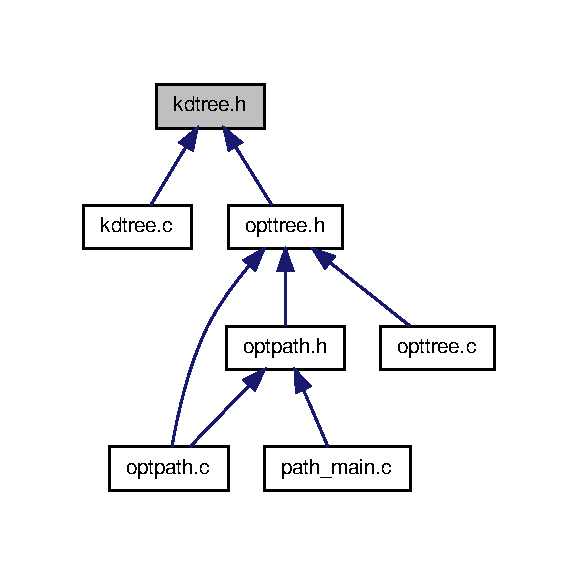
\includegraphics[width=277pt]{dc/de2/a00024}
\end{center}
\end{figure}
\subsection*{\-Functions}
\begin{DoxyCompactItemize}
\item 
struct \hyperlink{a00011}{kdtree} $\ast$ \hyperlink{a00014_a0267f17ca84a70322af662b16a625c16_a0267f17ca84a70322af662b16a625c16}{kd\-\_\-create} (int k)
\item 
void \hyperlink{a00014_aafdee4d5c129970e12fd9fe6da45d6d1_aafdee4d5c129970e12fd9fe6da45d6d1}{kd\-\_\-free} (struct \hyperlink{a00011}{kdtree} $\ast$tree)
\item 
void \hyperlink{a00014_a354bb35c5b031992cd0972dc53ad5d4f_a354bb35c5b031992cd0972dc53ad5d4f}{kd\-\_\-clear} (struct \hyperlink{a00011}{kdtree} $\ast$tree)
\item 
void \hyperlink{a00014_af2b7a413e4a0daf4add90cf982b954ec_af2b7a413e4a0daf4add90cf982b954ec}{kd\-\_\-data\-\_\-destructor} (struct \hyperlink{a00011}{kdtree} $\ast$tree, void($\ast$destr)(void $\ast$))
\item 
int \hyperlink{a00014_afafddbe0ccd0ca2c41917fb6d79f3392_afafddbe0ccd0ca2c41917fb6d79f3392}{kd\-\_\-insert} (struct \hyperlink{a00011}{kdtree} $\ast$tree, const double $\ast$pos, void $\ast$data)
\item 
int \hyperlink{a00014_ab64899a430280fc8affa205d82d07d10_ab64899a430280fc8affa205d82d07d10}{kd\-\_\-insertf} (struct \hyperlink{a00011}{kdtree} $\ast$tree, const float $\ast$pos, void $\ast$data)
\item 
int \hyperlink{a00014_a354954a360619c49f086402676b36e35_a354954a360619c49f086402676b36e35}{kd\-\_\-insert3} (struct \hyperlink{a00011}{kdtree} $\ast$tree, double x, double y, double z, void $\ast$data)
\item 
int \hyperlink{a00014_a9875b355df53d4545843f7471abb04f4_a9875b355df53d4545843f7471abb04f4}{kd\-\_\-insert3f} (struct \hyperlink{a00011}{kdtree} $\ast$tree, float x, float y, float z, void $\ast$data)
\item 
struct \hyperlink{a00010}{kdres} $\ast$ \hyperlink{a00014_a035f690066c2bd71caf4d38ff367a437_a035f690066c2bd71caf4d38ff367a437}{kd\-\_\-nearest} (struct \hyperlink{a00011}{kdtree} $\ast$tree, const double $\ast$pos)
\item 
struct \hyperlink{a00010}{kdres} $\ast$ \hyperlink{a00014_a62c3e2c5f4ee976a504d9e54080e332d_a62c3e2c5f4ee976a504d9e54080e332d}{kd\-\_\-nearestf} (struct \hyperlink{a00011}{kdtree} $\ast$tree, const float $\ast$pos)
\item 
struct \hyperlink{a00010}{kdres} $\ast$ \hyperlink{a00014_ad5d009b99e7804547508048f49b79d30_ad5d009b99e7804547508048f49b79d30}{kd\-\_\-nearest3} (struct \hyperlink{a00011}{kdtree} $\ast$tree, double x, double y, double z)
\item 
struct \hyperlink{a00010}{kdres} $\ast$ \hyperlink{a00014_a9811ac60c0e418bd5d0537e3a3568b6f_a9811ac60c0e418bd5d0537e3a3568b6f}{kd\-\_\-nearest3f} (struct \hyperlink{a00011}{kdtree} $\ast$tree, float x, float y, float z)
\item 
struct \hyperlink{a00010}{kdres} $\ast$ \hyperlink{a00014_ae7470d6cc3e640ff79c19fb60016763d_ae7470d6cc3e640ff79c19fb60016763d}{kd\-\_\-nearest\-\_\-range} (struct \hyperlink{a00011}{kdtree} $\ast$tree, const double $\ast$pos, double range)
\item 
struct \hyperlink{a00010}{kdres} $\ast$ \hyperlink{a00014_ac0425455c7c9b8b0a0058ab16d00b4a4_ac0425455c7c9b8b0a0058ab16d00b4a4}{kd\-\_\-nearest\-\_\-rangef} (struct \hyperlink{a00011}{kdtree} $\ast$tree, const float $\ast$pos, float range)
\item 
struct \hyperlink{a00010}{kdres} $\ast$ \hyperlink{a00014_a205361bbf9b2378819b17a1e101c1d23_a205361bbf9b2378819b17a1e101c1d23}{kd\-\_\-nearest\-\_\-range3} (struct \hyperlink{a00011}{kdtree} $\ast$tree, double x, double y, double z, double range)
\item 
struct \hyperlink{a00010}{kdres} $\ast$ \hyperlink{a00014_a31785d1b48d785e7c8f178a40671d4f4_a31785d1b48d785e7c8f178a40671d4f4}{kd\-\_\-nearest\-\_\-range3f} (struct \hyperlink{a00011}{kdtree} $\ast$tree, float x, float y, float z, float range)
\item 
void \hyperlink{a00014_ae783df8818133e4fb833e9203302f162_ae783df8818133e4fb833e9203302f162}{kd\-\_\-res\-\_\-free} (struct \hyperlink{a00010}{kdres} $\ast$set)
\item 
int \hyperlink{a00014_adb070dde37e9a978f231d730b7a24b53_adb070dde37e9a978f231d730b7a24b53}{kd\-\_\-res\-\_\-size} (struct \hyperlink{a00010}{kdres} $\ast$set)
\item 
void \hyperlink{a00014_a691ff69299aca39887ff3b4b2a0b81f6_a691ff69299aca39887ff3b4b2a0b81f6}{kd\-\_\-res\-\_\-rewind} (struct \hyperlink{a00010}{kdres} $\ast$set)
\item 
int \hyperlink{a00014_a9c331a704388b658a8c8fa779f6c4fe9_a9c331a704388b658a8c8fa779f6c4fe9}{kd\-\_\-res\-\_\-end} (struct \hyperlink{a00010}{kdres} $\ast$set)
\item 
int \hyperlink{a00014_ac2ef7750c902fd26a6d4e882e64df7f8_ac2ef7750c902fd26a6d4e882e64df7f8}{kd\-\_\-res\-\_\-next} (struct \hyperlink{a00010}{kdres} $\ast$set)
\item 
void $\ast$ \hyperlink{a00014_a5b0521aec4d2a2267bbab0f4408ec64a_a5b0521aec4d2a2267bbab0f4408ec64a}{kd\-\_\-res\-\_\-item} (struct \hyperlink{a00010}{kdres} $\ast$set, double $\ast$pos)
\item 
void $\ast$ \hyperlink{a00014_ae2d5802f669e14e245fc8ee6b8a3ff16_ae2d5802f669e14e245fc8ee6b8a3ff16}{kd\-\_\-res\-\_\-itemf} (struct \hyperlink{a00010}{kdres} $\ast$set, float $\ast$pos)
\item 
void $\ast$ \hyperlink{a00014_a68e3356de97626347762c20a1f29b493_a68e3356de97626347762c20a1f29b493}{kd\-\_\-res\-\_\-item3} (struct \hyperlink{a00010}{kdres} $\ast$set, double $\ast$x, double $\ast$y, double $\ast$z)
\item 
void $\ast$ \hyperlink{a00014_a09a99deb44dd60393a72dc91ab936e98_a09a99deb44dd60393a72dc91ab936e98}{kd\-\_\-res\-\_\-item3f} (struct \hyperlink{a00010}{kdres} $\ast$set, float $\ast$x, float $\ast$y, float $\ast$z)
\item 
void $\ast$ \hyperlink{a00014_abbff3a82caa304688020bc050d474d30_abbff3a82caa304688020bc050d474d30}{kd\-\_\-res\-\_\-item\-\_\-data} (struct \hyperlink{a00010}{kdres} $\ast$set)
\end{DoxyCompactItemize}


\subsection{\-Function \-Documentation}
\hypertarget{a00014_a354bb35c5b031992cd0972dc53ad5d4f_a354bb35c5b031992cd0972dc53ad5d4f}{\index{kdtree.\-h@{kdtree.\-h}!kd\-\_\-clear@{kd\-\_\-clear}}
\index{kd\-\_\-clear@{kd\-\_\-clear}!kdtree.h@{kdtree.\-h}}
\subsubsection[{kd\-\_\-clear}]{\setlength{\rightskip}{0pt plus 5cm}void {\bf kd\-\_\-clear} (
\begin{DoxyParamCaption}
\item[{struct {\bf kdtree} $\ast$}]{tree}
\end{DoxyParamCaption}
)}}\label{d2/de7/a00014_a354bb35c5b031992cd0972dc53ad5d4f_a354bb35c5b031992cd0972dc53ad5d4f}
\hypertarget{a00014_a0267f17ca84a70322af662b16a625c16_a0267f17ca84a70322af662b16a625c16}{\index{kdtree.\-h@{kdtree.\-h}!kd\-\_\-create@{kd\-\_\-create}}
\index{kd\-\_\-create@{kd\-\_\-create}!kdtree.h@{kdtree.\-h}}
\subsubsection[{kd\-\_\-create}]{\setlength{\rightskip}{0pt plus 5cm}struct {\bf kdtree}$\ast$ {\bf kd\-\_\-create} (
\begin{DoxyParamCaption}
\item[{int}]{k}
\end{DoxyParamCaption}
)\hspace{0.3cm}{\ttfamily  \mbox{[}read\mbox{]}}}}\label{d2/de7/a00014_a0267f17ca84a70322af662b16a625c16_a0267f17ca84a70322af662b16a625c16}
\hypertarget{a00014_af2b7a413e4a0daf4add90cf982b954ec_af2b7a413e4a0daf4add90cf982b954ec}{\index{kdtree.\-h@{kdtree.\-h}!kd\-\_\-data\-\_\-destructor@{kd\-\_\-data\-\_\-destructor}}
\index{kd\-\_\-data\-\_\-destructor@{kd\-\_\-data\-\_\-destructor}!kdtree.h@{kdtree.\-h}}
\subsubsection[{kd\-\_\-data\-\_\-destructor}]{\setlength{\rightskip}{0pt plus 5cm}void {\bf kd\-\_\-data\-\_\-destructor} (
\begin{DoxyParamCaption}
\item[{struct {\bf kdtree} $\ast$}]{tree, }
\item[{void($\ast$)(void $\ast$)}]{destr}
\end{DoxyParamCaption}
)}}\label{d2/de7/a00014_af2b7a413e4a0daf4add90cf982b954ec_af2b7a413e4a0daf4add90cf982b954ec}
\hypertarget{a00014_aafdee4d5c129970e12fd9fe6da45d6d1_aafdee4d5c129970e12fd9fe6da45d6d1}{\index{kdtree.\-h@{kdtree.\-h}!kd\-\_\-free@{kd\-\_\-free}}
\index{kd\-\_\-free@{kd\-\_\-free}!kdtree.h@{kdtree.\-h}}
\subsubsection[{kd\-\_\-free}]{\setlength{\rightskip}{0pt plus 5cm}void {\bf kd\-\_\-free} (
\begin{DoxyParamCaption}
\item[{struct {\bf kdtree} $\ast$}]{tree}
\end{DoxyParamCaption}
)}}\label{d2/de7/a00014_aafdee4d5c129970e12fd9fe6da45d6d1_aafdee4d5c129970e12fd9fe6da45d6d1}
\hypertarget{a00014_afafddbe0ccd0ca2c41917fb6d79f3392_afafddbe0ccd0ca2c41917fb6d79f3392}{\index{kdtree.\-h@{kdtree.\-h}!kd\-\_\-insert@{kd\-\_\-insert}}
\index{kd\-\_\-insert@{kd\-\_\-insert}!kdtree.h@{kdtree.\-h}}
\subsubsection[{kd\-\_\-insert}]{\setlength{\rightskip}{0pt plus 5cm}int {\bf kd\-\_\-insert} (
\begin{DoxyParamCaption}
\item[{struct {\bf kdtree} $\ast$}]{tree, }
\item[{const double $\ast$}]{pos, }
\item[{void $\ast$}]{data}
\end{DoxyParamCaption}
)}}\label{d2/de7/a00014_afafddbe0ccd0ca2c41917fb6d79f3392_afafddbe0ccd0ca2c41917fb6d79f3392}
\hypertarget{a00014_a354954a360619c49f086402676b36e35_a354954a360619c49f086402676b36e35}{\index{kdtree.\-h@{kdtree.\-h}!kd\-\_\-insert3@{kd\-\_\-insert3}}
\index{kd\-\_\-insert3@{kd\-\_\-insert3}!kdtree.h@{kdtree.\-h}}
\subsubsection[{kd\-\_\-insert3}]{\setlength{\rightskip}{0pt plus 5cm}int {\bf kd\-\_\-insert3} (
\begin{DoxyParamCaption}
\item[{struct {\bf kdtree} $\ast$}]{tree, }
\item[{double}]{x, }
\item[{double}]{y, }
\item[{double}]{z, }
\item[{void $\ast$}]{data}
\end{DoxyParamCaption}
)}}\label{d2/de7/a00014_a354954a360619c49f086402676b36e35_a354954a360619c49f086402676b36e35}
\hypertarget{a00014_a9875b355df53d4545843f7471abb04f4_a9875b355df53d4545843f7471abb04f4}{\index{kdtree.\-h@{kdtree.\-h}!kd\-\_\-insert3f@{kd\-\_\-insert3f}}
\index{kd\-\_\-insert3f@{kd\-\_\-insert3f}!kdtree.h@{kdtree.\-h}}
\subsubsection[{kd\-\_\-insert3f}]{\setlength{\rightskip}{0pt plus 5cm}int {\bf kd\-\_\-insert3f} (
\begin{DoxyParamCaption}
\item[{struct {\bf kdtree} $\ast$}]{tree, }
\item[{float}]{x, }
\item[{float}]{y, }
\item[{float}]{z, }
\item[{void $\ast$}]{data}
\end{DoxyParamCaption}
)}}\label{d2/de7/a00014_a9875b355df53d4545843f7471abb04f4_a9875b355df53d4545843f7471abb04f4}
\hypertarget{a00014_ab64899a430280fc8affa205d82d07d10_ab64899a430280fc8affa205d82d07d10}{\index{kdtree.\-h@{kdtree.\-h}!kd\-\_\-insertf@{kd\-\_\-insertf}}
\index{kd\-\_\-insertf@{kd\-\_\-insertf}!kdtree.h@{kdtree.\-h}}
\subsubsection[{kd\-\_\-insertf}]{\setlength{\rightskip}{0pt plus 5cm}int {\bf kd\-\_\-insertf} (
\begin{DoxyParamCaption}
\item[{struct {\bf kdtree} $\ast$}]{tree, }
\item[{const float $\ast$}]{pos, }
\item[{void $\ast$}]{data}
\end{DoxyParamCaption}
)}}\label{d2/de7/a00014_ab64899a430280fc8affa205d82d07d10_ab64899a430280fc8affa205d82d07d10}
\hypertarget{a00014_a035f690066c2bd71caf4d38ff367a437_a035f690066c2bd71caf4d38ff367a437}{\index{kdtree.\-h@{kdtree.\-h}!kd\-\_\-nearest@{kd\-\_\-nearest}}
\index{kd\-\_\-nearest@{kd\-\_\-nearest}!kdtree.h@{kdtree.\-h}}
\subsubsection[{kd\-\_\-nearest}]{\setlength{\rightskip}{0pt plus 5cm}struct {\bf kdres}$\ast$ {\bf kd\-\_\-nearest} (
\begin{DoxyParamCaption}
\item[{struct {\bf kdtree} $\ast$}]{tree, }
\item[{const double $\ast$}]{pos}
\end{DoxyParamCaption}
)\hspace{0.3cm}{\ttfamily  \mbox{[}read\mbox{]}}}}\label{d2/de7/a00014_a035f690066c2bd71caf4d38ff367a437_a035f690066c2bd71caf4d38ff367a437}
\hypertarget{a00014_ad5d009b99e7804547508048f49b79d30_ad5d009b99e7804547508048f49b79d30}{\index{kdtree.\-h@{kdtree.\-h}!kd\-\_\-nearest3@{kd\-\_\-nearest3}}
\index{kd\-\_\-nearest3@{kd\-\_\-nearest3}!kdtree.h@{kdtree.\-h}}
\subsubsection[{kd\-\_\-nearest3}]{\setlength{\rightskip}{0pt plus 5cm}struct {\bf kdres}$\ast$ {\bf kd\-\_\-nearest3} (
\begin{DoxyParamCaption}
\item[{struct {\bf kdtree} $\ast$}]{tree, }
\item[{double}]{x, }
\item[{double}]{y, }
\item[{double}]{z}
\end{DoxyParamCaption}
)\hspace{0.3cm}{\ttfamily  \mbox{[}read\mbox{]}}}}\label{d2/de7/a00014_ad5d009b99e7804547508048f49b79d30_ad5d009b99e7804547508048f49b79d30}
\hypertarget{a00014_a9811ac60c0e418bd5d0537e3a3568b6f_a9811ac60c0e418bd5d0537e3a3568b6f}{\index{kdtree.\-h@{kdtree.\-h}!kd\-\_\-nearest3f@{kd\-\_\-nearest3f}}
\index{kd\-\_\-nearest3f@{kd\-\_\-nearest3f}!kdtree.h@{kdtree.\-h}}
\subsubsection[{kd\-\_\-nearest3f}]{\setlength{\rightskip}{0pt plus 5cm}struct {\bf kdres}$\ast$ {\bf kd\-\_\-nearest3f} (
\begin{DoxyParamCaption}
\item[{struct {\bf kdtree} $\ast$}]{tree, }
\item[{float}]{x, }
\item[{float}]{y, }
\item[{float}]{z}
\end{DoxyParamCaption}
)\hspace{0.3cm}{\ttfamily  \mbox{[}read\mbox{]}}}}\label{d2/de7/a00014_a9811ac60c0e418bd5d0537e3a3568b6f_a9811ac60c0e418bd5d0537e3a3568b6f}
\hypertarget{a00014_ae7470d6cc3e640ff79c19fb60016763d_ae7470d6cc3e640ff79c19fb60016763d}{\index{kdtree.\-h@{kdtree.\-h}!kd\-\_\-nearest\-\_\-range@{kd\-\_\-nearest\-\_\-range}}
\index{kd\-\_\-nearest\-\_\-range@{kd\-\_\-nearest\-\_\-range}!kdtree.h@{kdtree.\-h}}
\subsubsection[{kd\-\_\-nearest\-\_\-range}]{\setlength{\rightskip}{0pt plus 5cm}struct {\bf kdres}$\ast$ {\bf kd\-\_\-nearest\-\_\-range} (
\begin{DoxyParamCaption}
\item[{struct {\bf kdtree} $\ast$}]{tree, }
\item[{const double $\ast$}]{pos, }
\item[{double}]{range}
\end{DoxyParamCaption}
)\hspace{0.3cm}{\ttfamily  \mbox{[}read\mbox{]}}}}\label{d2/de7/a00014_ae7470d6cc3e640ff79c19fb60016763d_ae7470d6cc3e640ff79c19fb60016763d}
\hypertarget{a00014_a205361bbf9b2378819b17a1e101c1d23_a205361bbf9b2378819b17a1e101c1d23}{\index{kdtree.\-h@{kdtree.\-h}!kd\-\_\-nearest\-\_\-range3@{kd\-\_\-nearest\-\_\-range3}}
\index{kd\-\_\-nearest\-\_\-range3@{kd\-\_\-nearest\-\_\-range3}!kdtree.h@{kdtree.\-h}}
\subsubsection[{kd\-\_\-nearest\-\_\-range3}]{\setlength{\rightskip}{0pt plus 5cm}struct {\bf kdres}$\ast$ {\bf kd\-\_\-nearest\-\_\-range3} (
\begin{DoxyParamCaption}
\item[{struct {\bf kdtree} $\ast$}]{tree, }
\item[{double}]{x, }
\item[{double}]{y, }
\item[{double}]{z, }
\item[{double}]{range}
\end{DoxyParamCaption}
)\hspace{0.3cm}{\ttfamily  \mbox{[}read\mbox{]}}}}\label{d2/de7/a00014_a205361bbf9b2378819b17a1e101c1d23_a205361bbf9b2378819b17a1e101c1d23}
\hypertarget{a00014_a31785d1b48d785e7c8f178a40671d4f4_a31785d1b48d785e7c8f178a40671d4f4}{\index{kdtree.\-h@{kdtree.\-h}!kd\-\_\-nearest\-\_\-range3f@{kd\-\_\-nearest\-\_\-range3f}}
\index{kd\-\_\-nearest\-\_\-range3f@{kd\-\_\-nearest\-\_\-range3f}!kdtree.h@{kdtree.\-h}}
\subsubsection[{kd\-\_\-nearest\-\_\-range3f}]{\setlength{\rightskip}{0pt plus 5cm}struct {\bf kdres}$\ast$ {\bf kd\-\_\-nearest\-\_\-range3f} (
\begin{DoxyParamCaption}
\item[{struct {\bf kdtree} $\ast$}]{tree, }
\item[{float}]{x, }
\item[{float}]{y, }
\item[{float}]{z, }
\item[{float}]{range}
\end{DoxyParamCaption}
)\hspace{0.3cm}{\ttfamily  \mbox{[}read\mbox{]}}}}\label{d2/de7/a00014_a31785d1b48d785e7c8f178a40671d4f4_a31785d1b48d785e7c8f178a40671d4f4}
\hypertarget{a00014_ac0425455c7c9b8b0a0058ab16d00b4a4_ac0425455c7c9b8b0a0058ab16d00b4a4}{\index{kdtree.\-h@{kdtree.\-h}!kd\-\_\-nearest\-\_\-rangef@{kd\-\_\-nearest\-\_\-rangef}}
\index{kd\-\_\-nearest\-\_\-rangef@{kd\-\_\-nearest\-\_\-rangef}!kdtree.h@{kdtree.\-h}}
\subsubsection[{kd\-\_\-nearest\-\_\-rangef}]{\setlength{\rightskip}{0pt plus 5cm}struct {\bf kdres}$\ast$ {\bf kd\-\_\-nearest\-\_\-rangef} (
\begin{DoxyParamCaption}
\item[{struct {\bf kdtree} $\ast$}]{tree, }
\item[{const float $\ast$}]{pos, }
\item[{float}]{range}
\end{DoxyParamCaption}
)\hspace{0.3cm}{\ttfamily  \mbox{[}read\mbox{]}}}}\label{d2/de7/a00014_ac0425455c7c9b8b0a0058ab16d00b4a4_ac0425455c7c9b8b0a0058ab16d00b4a4}
\hypertarget{a00014_a62c3e2c5f4ee976a504d9e54080e332d_a62c3e2c5f4ee976a504d9e54080e332d}{\index{kdtree.\-h@{kdtree.\-h}!kd\-\_\-nearestf@{kd\-\_\-nearestf}}
\index{kd\-\_\-nearestf@{kd\-\_\-nearestf}!kdtree.h@{kdtree.\-h}}
\subsubsection[{kd\-\_\-nearestf}]{\setlength{\rightskip}{0pt plus 5cm}struct {\bf kdres}$\ast$ {\bf kd\-\_\-nearestf} (
\begin{DoxyParamCaption}
\item[{struct {\bf kdtree} $\ast$}]{tree, }
\item[{const float $\ast$}]{pos}
\end{DoxyParamCaption}
)\hspace{0.3cm}{\ttfamily  \mbox{[}read\mbox{]}}}}\label{d2/de7/a00014_a62c3e2c5f4ee976a504d9e54080e332d_a62c3e2c5f4ee976a504d9e54080e332d}
\hypertarget{a00014_a9c331a704388b658a8c8fa779f6c4fe9_a9c331a704388b658a8c8fa779f6c4fe9}{\index{kdtree.\-h@{kdtree.\-h}!kd\-\_\-res\-\_\-end@{kd\-\_\-res\-\_\-end}}
\index{kd\-\_\-res\-\_\-end@{kd\-\_\-res\-\_\-end}!kdtree.h@{kdtree.\-h}}
\subsubsection[{kd\-\_\-res\-\_\-end}]{\setlength{\rightskip}{0pt plus 5cm}int {\bf kd\-\_\-res\-\_\-end} (
\begin{DoxyParamCaption}
\item[{struct {\bf kdres} $\ast$}]{set}
\end{DoxyParamCaption}
)}}\label{d2/de7/a00014_a9c331a704388b658a8c8fa779f6c4fe9_a9c331a704388b658a8c8fa779f6c4fe9}
\hypertarget{a00014_ae783df8818133e4fb833e9203302f162_ae783df8818133e4fb833e9203302f162}{\index{kdtree.\-h@{kdtree.\-h}!kd\-\_\-res\-\_\-free@{kd\-\_\-res\-\_\-free}}
\index{kd\-\_\-res\-\_\-free@{kd\-\_\-res\-\_\-free}!kdtree.h@{kdtree.\-h}}
\subsubsection[{kd\-\_\-res\-\_\-free}]{\setlength{\rightskip}{0pt plus 5cm}void {\bf kd\-\_\-res\-\_\-free} (
\begin{DoxyParamCaption}
\item[{struct {\bf kdres} $\ast$}]{set}
\end{DoxyParamCaption}
)}}\label{d2/de7/a00014_ae783df8818133e4fb833e9203302f162_ae783df8818133e4fb833e9203302f162}
\hypertarget{a00014_a5b0521aec4d2a2267bbab0f4408ec64a_a5b0521aec4d2a2267bbab0f4408ec64a}{\index{kdtree.\-h@{kdtree.\-h}!kd\-\_\-res\-\_\-item@{kd\-\_\-res\-\_\-item}}
\index{kd\-\_\-res\-\_\-item@{kd\-\_\-res\-\_\-item}!kdtree.h@{kdtree.\-h}}
\subsubsection[{kd\-\_\-res\-\_\-item}]{\setlength{\rightskip}{0pt plus 5cm}void$\ast$ {\bf kd\-\_\-res\-\_\-item} (
\begin{DoxyParamCaption}
\item[{struct {\bf kdres} $\ast$}]{set, }
\item[{double $\ast$}]{pos}
\end{DoxyParamCaption}
)}}\label{d2/de7/a00014_a5b0521aec4d2a2267bbab0f4408ec64a_a5b0521aec4d2a2267bbab0f4408ec64a}
\hypertarget{a00014_a68e3356de97626347762c20a1f29b493_a68e3356de97626347762c20a1f29b493}{\index{kdtree.\-h@{kdtree.\-h}!kd\-\_\-res\-\_\-item3@{kd\-\_\-res\-\_\-item3}}
\index{kd\-\_\-res\-\_\-item3@{kd\-\_\-res\-\_\-item3}!kdtree.h@{kdtree.\-h}}
\subsubsection[{kd\-\_\-res\-\_\-item3}]{\setlength{\rightskip}{0pt plus 5cm}void$\ast$ {\bf kd\-\_\-res\-\_\-item3} (
\begin{DoxyParamCaption}
\item[{struct {\bf kdres} $\ast$}]{set, }
\item[{double $\ast$}]{x, }
\item[{double $\ast$}]{y, }
\item[{double $\ast$}]{z}
\end{DoxyParamCaption}
)}}\label{d2/de7/a00014_a68e3356de97626347762c20a1f29b493_a68e3356de97626347762c20a1f29b493}
\hypertarget{a00014_a09a99deb44dd60393a72dc91ab936e98_a09a99deb44dd60393a72dc91ab936e98}{\index{kdtree.\-h@{kdtree.\-h}!kd\-\_\-res\-\_\-item3f@{kd\-\_\-res\-\_\-item3f}}
\index{kd\-\_\-res\-\_\-item3f@{kd\-\_\-res\-\_\-item3f}!kdtree.h@{kdtree.\-h}}
\subsubsection[{kd\-\_\-res\-\_\-item3f}]{\setlength{\rightskip}{0pt plus 5cm}void$\ast$ {\bf kd\-\_\-res\-\_\-item3f} (
\begin{DoxyParamCaption}
\item[{struct {\bf kdres} $\ast$}]{set, }
\item[{float $\ast$}]{x, }
\item[{float $\ast$}]{y, }
\item[{float $\ast$}]{z}
\end{DoxyParamCaption}
)}}\label{d2/de7/a00014_a09a99deb44dd60393a72dc91ab936e98_a09a99deb44dd60393a72dc91ab936e98}
\hypertarget{a00014_abbff3a82caa304688020bc050d474d30_abbff3a82caa304688020bc050d474d30}{\index{kdtree.\-h@{kdtree.\-h}!kd\-\_\-res\-\_\-item\-\_\-data@{kd\-\_\-res\-\_\-item\-\_\-data}}
\index{kd\-\_\-res\-\_\-item\-\_\-data@{kd\-\_\-res\-\_\-item\-\_\-data}!kdtree.h@{kdtree.\-h}}
\subsubsection[{kd\-\_\-res\-\_\-item\-\_\-data}]{\setlength{\rightskip}{0pt plus 5cm}void$\ast$ {\bf kd\-\_\-res\-\_\-item\-\_\-data} (
\begin{DoxyParamCaption}
\item[{struct {\bf kdres} $\ast$}]{set}
\end{DoxyParamCaption}
)}}\label{d2/de7/a00014_abbff3a82caa304688020bc050d474d30_abbff3a82caa304688020bc050d474d30}
\hypertarget{a00014_ae2d5802f669e14e245fc8ee6b8a3ff16_ae2d5802f669e14e245fc8ee6b8a3ff16}{\index{kdtree.\-h@{kdtree.\-h}!kd\-\_\-res\-\_\-itemf@{kd\-\_\-res\-\_\-itemf}}
\index{kd\-\_\-res\-\_\-itemf@{kd\-\_\-res\-\_\-itemf}!kdtree.h@{kdtree.\-h}}
\subsubsection[{kd\-\_\-res\-\_\-itemf}]{\setlength{\rightskip}{0pt plus 5cm}void$\ast$ {\bf kd\-\_\-res\-\_\-itemf} (
\begin{DoxyParamCaption}
\item[{struct {\bf kdres} $\ast$}]{set, }
\item[{float $\ast$}]{pos}
\end{DoxyParamCaption}
)}}\label{d2/de7/a00014_ae2d5802f669e14e245fc8ee6b8a3ff16_ae2d5802f669e14e245fc8ee6b8a3ff16}
\hypertarget{a00014_ac2ef7750c902fd26a6d4e882e64df7f8_ac2ef7750c902fd26a6d4e882e64df7f8}{\index{kdtree.\-h@{kdtree.\-h}!kd\-\_\-res\-\_\-next@{kd\-\_\-res\-\_\-next}}
\index{kd\-\_\-res\-\_\-next@{kd\-\_\-res\-\_\-next}!kdtree.h@{kdtree.\-h}}
\subsubsection[{kd\-\_\-res\-\_\-next}]{\setlength{\rightskip}{0pt plus 5cm}int {\bf kd\-\_\-res\-\_\-next} (
\begin{DoxyParamCaption}
\item[{struct {\bf kdres} $\ast$}]{set}
\end{DoxyParamCaption}
)}}\label{d2/de7/a00014_ac2ef7750c902fd26a6d4e882e64df7f8_ac2ef7750c902fd26a6d4e882e64df7f8}
\hypertarget{a00014_a691ff69299aca39887ff3b4b2a0b81f6_a691ff69299aca39887ff3b4b2a0b81f6}{\index{kdtree.\-h@{kdtree.\-h}!kd\-\_\-res\-\_\-rewind@{kd\-\_\-res\-\_\-rewind}}
\index{kd\-\_\-res\-\_\-rewind@{kd\-\_\-res\-\_\-rewind}!kdtree.h@{kdtree.\-h}}
\subsubsection[{kd\-\_\-res\-\_\-rewind}]{\setlength{\rightskip}{0pt plus 5cm}void {\bf kd\-\_\-res\-\_\-rewind} (
\begin{DoxyParamCaption}
\item[{struct {\bf kdres} $\ast$}]{set}
\end{DoxyParamCaption}
)}}\label{d2/de7/a00014_a691ff69299aca39887ff3b4b2a0b81f6_a691ff69299aca39887ff3b4b2a0b81f6}
\hypertarget{a00014_adb070dde37e9a978f231d730b7a24b53_adb070dde37e9a978f231d730b7a24b53}{\index{kdtree.\-h@{kdtree.\-h}!kd\-\_\-res\-\_\-size@{kd\-\_\-res\-\_\-size}}
\index{kd\-\_\-res\-\_\-size@{kd\-\_\-res\-\_\-size}!kdtree.h@{kdtree.\-h}}
\subsubsection[{kd\-\_\-res\-\_\-size}]{\setlength{\rightskip}{0pt plus 5cm}int {\bf kd\-\_\-res\-\_\-size} (
\begin{DoxyParamCaption}
\item[{struct {\bf kdres} $\ast$}]{set}
\end{DoxyParamCaption}
)}}\label{d2/de7/a00014_adb070dde37e9a978f231d730b7a24b53_adb070dde37e9a978f231d730b7a24b53}

\hypertarget{a00015}{\section{optpath.\-c \-File \-Reference}
\label{dd/d1b/a00015}\index{optpath.\-c@{optpath.\-c}}
}
{\ttfamily \#include $<$stdlib.\-h$>$}\*
{\ttfamily \#include $<$stdio.\-h$>$}\*
{\ttfamily \#include $<$math.\-h$>$}\*
{\ttfamily \#include $<$glib.\-h$>$}\*
{\ttfamily \#include $<$sys/time.\-h$>$}\*
{\ttfamily \#include $<$unistd.\-h$>$}\*
{\ttfamily \#include \char`\"{}optpath.\-h\char`\"{}}\*
{\ttfamily \#include \char`\"{}opttree.\-h\char`\"{}}\*
{\ttfamily \#include \char`\"{}geos\-\_\-c.\-h\char`\"{}}\*
{\ttfamily \#include \char`\"{}/usr/include/json/json.\-h\char`\"{}}\*
\-Include dependency graph for optpath.\-c\-:
\nopagebreak
\begin{figure}[H]
\begin{center}
\leavevmode
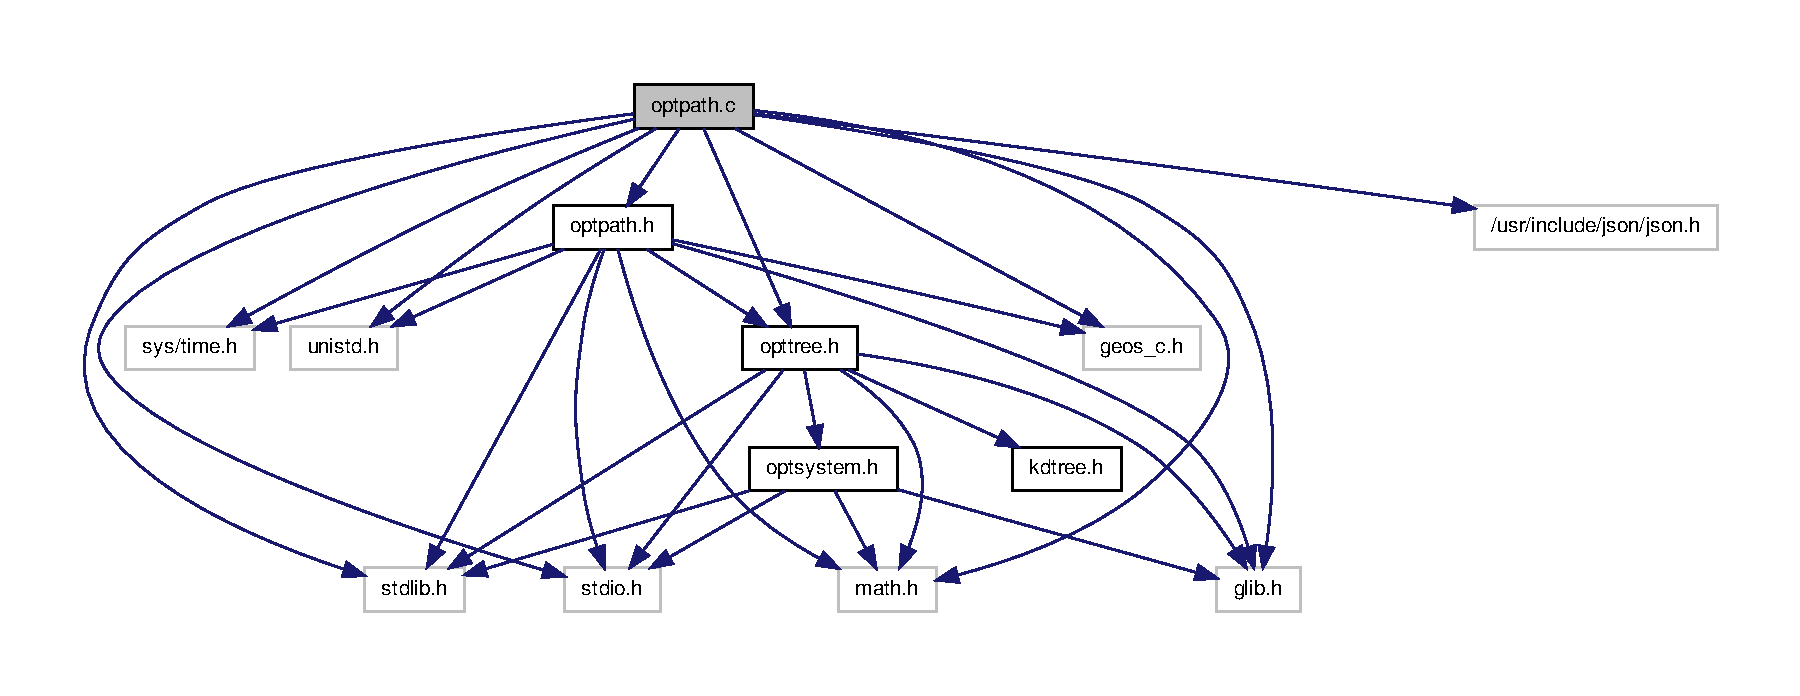
\includegraphics[width=350pt]{d3/dfe/a00025}
\end{center}
\end{figure}
\subsection*{\-Functions}
\begin{DoxyCompactItemize}
\item 
int64\-\_\-t \hyperlink{a00015_a7a93270b029dd7f09ac421ff7a473cd9_a7a93270b029dd7f09ac421ff7a473cd9}{ts\-\_\-now} ()
\item 
void \hyperlink{a00015_abb72a9e5586947ffa14de7aea6c8d7b4_abb72a9e5586947ffa14de7aea6c8d7b4}{notice1} (const char $\ast$fmt,...)
\item 
void \hyperlink{a00015_ab369473e6f056b28d426c97004c47828_ab369473e6f056b28d426c97004c47828}{log\-\_\-and\-\_\-exit1} (const char $\ast$fmt,...)
\item 
\hyperlink{a00016_a5f269c22e6d9d32b0b0ad7e6166854df_a5f269c22e6d9d32b0b0ad7e6166854df}{location} \hyperlink{a00015_a8fccd24d5b565d686f8ffd2820bf372a_a8fccd24d5b565d686f8ffd2820bf372a}{locat\-\_\-point} (double x, double y)
\begin{DoxyCompactList}\small\item\em find the location of a given point \end{DoxyCompactList}\item 
\-G\-S\-List $\ast$ \hyperlink{a00015_a25f1e769fb021e10c7a6923f56ab4f46_a25f1e769fb021e10c7a6923f56ab4f46}{dividing\-\_\-path} (double x1, double y1, double x2, double y2, char $\ast$obstacle, \hyperlink{a00016_a5f269c22e6d9d32b0b0ad7e6166854df_a5f269c22e6d9d32b0b0ad7e6166854df}{location} loc)
\begin{DoxyCompactList}\small\item\em \-This function is used when one of the daparture or arrival point is situated in one of the complex area already defined. \end{DoxyCompactList}\item 
int \hyperlink{a00015_abbed0c74429bd1201c2d98acfb81371e_abbed0c74429bd1201c2d98acfb81371e}{final\-\_\-path} (double x\-\_\-root, double y\-\_\-root, double x\-\_\-arrival, double y\-\_\-arrival, char $\ast$obstacle)
\begin{DoxyCompactList}\small\item\em \-This function calculate the final path that could be a connexion between 2 paths, then it fill the geojson file of the trajectory. \end{DoxyCompactList}\item 
\hyperlink{a00020_a07b75293fafb6f31b7e9f723848ad105_a07b75293fafb6f31b7e9f723848ad105}{opttree\-\_\-t} $\ast$ \hyperlink{a00015_a55d37159a13f40fdb4d2bda4b8a4c599_a55d37159a13f40fdb4d2bda4b8a4c599}{create\-\_\-environnement} (double x\-\_\-root, double y\-\_\-root, double x\-\_\-arrival, double y\-\_\-arrival, char $\ast$obstacle, int k)
\begin{DoxyCompactList}\small\item\em create the work environement; actually root\-\_\-state, goal\-\_\-region, operating region(depending on departure and arrival) and obstacle list(continents) \end{DoxyCompactList}\item 
\-G\-S\-List $\ast$ \hyperlink{a00015_afbf6f731092d290f20929a518bdf00c3_afbf6f731092d290f20929a518bdf00c3}{path} (double x\-\_\-root, double y\-\_\-root, double x\-\_\-arrival, double y\-\_\-arrival, char $\ast$obstacle)
\begin{DoxyCompactList}\small\item\em \-This function calculate the shortest path between two points\-: applicate rrtstar alogorithm, then use the correcting path algorithm to affinate the result. \end{DoxyCompactList}\item 
\-G\-S\-List $\ast$ \hyperlink{a00015_ada3d9a3dfb21481abb2ba7c5afa22809_ada3d9a3dfb21481abb2ba7c5afa22809}{correcting\-\_\-path} (\hyperlink{a00020_a07b75293fafb6f31b7e9f723848ad105_a07b75293fafb6f31b7e9f723848ad105}{opttree\-\_\-t} $\ast$opttree, \-G\-S\-List $\ast$optstates\-\_\-list, int k)
\begin{DoxyCompactList}\small\item\em from a path between two points (the result of rrtstar algorithm but with minimum number of iterations), make a better one by eleminating nodes and adding others \end{DoxyCompactList}\end{DoxyCompactItemize}


\subsection{\-Function \-Documentation}
\hypertarget{a00015_ada3d9a3dfb21481abb2ba7c5afa22809_ada3d9a3dfb21481abb2ba7c5afa22809}{\index{optpath.\-c@{optpath.\-c}!correcting\-\_\-path@{correcting\-\_\-path}}
\index{correcting\-\_\-path@{correcting\-\_\-path}!optpath.c@{optpath.\-c}}
\subsubsection[{correcting\-\_\-path}]{\setlength{\rightskip}{0pt plus 5cm}\-G\-S\-List $\ast$ {\bf correcting\-\_\-path} (
\begin{DoxyParamCaption}
\item[{{\bf opttree\-\_\-t} $\ast$}]{opttree, }
\item[{\-G\-S\-List $\ast$}]{optstates\-\_\-list, }
\item[{int}]{k}
\end{DoxyParamCaption}
)}}\label{dd/d1b/a00015_ada3d9a3dfb21481abb2ba7c5afa22809_ada3d9a3dfb21481abb2ba7c5afa22809}


from a path between two points (the result of rrtstar algorithm but with minimum number of iterations), make a better one by eleminating nodes and adding others 


\begin{DoxyParams}{\-Parameters}
{\em opttree} & the opttree\-\_\-t structure already created (the environnement of working) \\
\hline
{\em optstates\-\_\-list} & the list of nodes constituting the rrtstar path \\
\hline
{\em k} & compressing factor \\
\hline
\end{DoxyParams}
\begin{DoxyReturn}{\-Returns}
list\-\_\-ptr a \-G\-S\-List containing the states that constitute the new better path 
\end{DoxyReturn}
\hypertarget{a00015_a55d37159a13f40fdb4d2bda4b8a4c599_a55d37159a13f40fdb4d2bda4b8a4c599}{\index{optpath.\-c@{optpath.\-c}!create\-\_\-environnement@{create\-\_\-environnement}}
\index{create\-\_\-environnement@{create\-\_\-environnement}!optpath.c@{optpath.\-c}}
\subsubsection[{create\-\_\-environnement}]{\setlength{\rightskip}{0pt plus 5cm}{\bf opttree\-\_\-t} $\ast$ {\bf create\-\_\-environnement} (
\begin{DoxyParamCaption}
\item[{double}]{x\-\_\-root, }
\item[{double}]{y\-\_\-root, }
\item[{double}]{x\-\_\-arrival, }
\item[{double}]{y\-\_\-arrival, }
\item[{char $\ast$}]{obstacle, }
\item[{int}]{k}
\end{DoxyParamCaption}
)}}\label{dd/d1b/a00015_a55d37159a13f40fdb4d2bda4b8a4c599_a55d37159a13f40fdb4d2bda4b8a4c599}


create the work environement; actually root\-\_\-state, goal\-\_\-region, operating region(depending on departure and arrival) and obstacle list(continents) 


\begin{DoxyParams}{\-Parameters}
{\em x\-\_\-root} & the x-\/coordinate of the departure point \\
\hline
{\em y\-\_\-root} & the y-\/coordinate of the departure point \\
\hline
{\em x\-\_\-arrival} & the x-\/coordinate of the arrival point \\
\hline
{\em y\-\_\-arrival} & the y-\/coordinate of the arrival point \\
\hline
{\em obstacles} & the name of the obstacles file \\
\hline
{\em k} & the factor of compressing the operating region. \-In fact, if we work on all planisphere we compresse it in order to increase the number of point randomized \\
\hline
\end{DoxyParams}
\begin{DoxyReturn}{\-Returns}
1 if the path has been found, else 0 
\end{DoxyReturn}
\hypertarget{a00015_a25f1e769fb021e10c7a6923f56ab4f46_a25f1e769fb021e10c7a6923f56ab4f46}{\index{optpath.\-c@{optpath.\-c}!dividing\-\_\-path@{dividing\-\_\-path}}
\index{dividing\-\_\-path@{dividing\-\_\-path}!optpath.c@{optpath.\-c}}
\subsubsection[{dividing\-\_\-path}]{\setlength{\rightskip}{0pt plus 5cm}\-G\-S\-List $\ast$ {\bf dividing\-\_\-path} (
\begin{DoxyParamCaption}
\item[{double}]{x1, }
\item[{double}]{y1, }
\item[{double}]{x2, }
\item[{double}]{y2, }
\item[{char $\ast$}]{obstacle, }
\item[{{\bf location}}]{loc}
\end{DoxyParamCaption}
)}}\label{dd/d1b/a00015_a25f1e769fb021e10c7a6923f56ab4f46_a25f1e769fb021e10c7a6923f56ab4f46}


\-This function is used when one of the daparture or arrival point is situated in one of the complex area already defined. 


\begin{DoxyParams}{\-Parameters}
{\em x1} & the x-\/coordinate of the departure point \\
\hline
{\em y1} & the y-\/coordinate of the departure point \\
\hline
{\em x2} & the x-\/coordinate of the arrival point \\
\hline
{\em y2} & the y-\/coordinate of the arrival point \\
\hline
{\em obstacle} & the name of the obstacles file \\
\hline
{\em loc} & location of the unordinary point \\
\hline
\end{DoxyParams}
\begin{DoxyReturn}{\-Returns}
list\-\_\-ptr a \-G\-S\-List containing the states that constitute the path 
\end{DoxyReturn}
\hypertarget{a00015_abbed0c74429bd1201c2d98acfb81371e_abbed0c74429bd1201c2d98acfb81371e}{\index{optpath.\-c@{optpath.\-c}!final\-\_\-path@{final\-\_\-path}}
\index{final\-\_\-path@{final\-\_\-path}!optpath.c@{optpath.\-c}}
\subsubsection[{final\-\_\-path}]{\setlength{\rightskip}{0pt plus 5cm}int {\bf final\-\_\-path} (
\begin{DoxyParamCaption}
\item[{double}]{x\-\_\-root, }
\item[{double}]{y\-\_\-root, }
\item[{double}]{x\-\_\-arrival, }
\item[{double}]{y\-\_\-arrival, }
\item[{char $\ast$}]{obstacle}
\end{DoxyParamCaption}
)}}\label{dd/d1b/a00015_abbed0c74429bd1201c2d98acfb81371e_abbed0c74429bd1201c2d98acfb81371e}


\-This function calculate the final path that could be a connexion between 2 paths, then it fill the geojson file of the trajectory. 


\begin{DoxyParams}{\-Parameters}
{\em x\-\_\-root} & the x-\/coordinate of the departure point \\
\hline
{\em y\-\_\-root} & the y-\/coordinate of the departure point \\
\hline
{\em x\-\_\-arrival} & the x-\/coordinate of the arrival point \\
\hline
{\em y\-\_\-arrival} & the y-\/coordinate of the arrival point \\
\hline
{\em obstacle} & the name of the obstacles file \\
\hline
\end{DoxyParams}
\begin{DoxyReturn}{\-Returns}
1 if the path has been found, else 0 
\end{DoxyReturn}
\hypertarget{a00015_a8fccd24d5b565d686f8ffd2820bf372a_a8fccd24d5b565d686f8ffd2820bf372a}{\index{optpath.\-c@{optpath.\-c}!locat\-\_\-point@{locat\-\_\-point}}
\index{locat\-\_\-point@{locat\-\_\-point}!optpath.c@{optpath.\-c}}
\subsubsection[{locat\-\_\-point}]{\setlength{\rightskip}{0pt plus 5cm}{\bf location} {\bf locat\-\_\-point} (
\begin{DoxyParamCaption}
\item[{double}]{x, }
\item[{double}]{y}
\end{DoxyParamCaption}
)}}\label{dd/d1b/a00015_a8fccd24d5b565d686f8ffd2820bf372a_a8fccd24d5b565d686f8ffd2820bf372a}


find the location of a given point 


\begin{DoxyParams}{\-Parameters}
{\em x} & the x-\/coordinate of the point \\
\hline
{\em y} & the y-\/coordinate of the point \\
\hline
\end{DoxyParams}
\begin{DoxyReturn}{\-Returns}
loc the location if the point is in a particular area, else \-O\-R\-D\-I\-N\-A\-R\-Y 
\end{DoxyReturn}
\hypertarget{a00015_ab369473e6f056b28d426c97004c47828_ab369473e6f056b28d426c97004c47828}{\index{optpath.\-c@{optpath.\-c}!log\-\_\-and\-\_\-exit1@{log\-\_\-and\-\_\-exit1}}
\index{log\-\_\-and\-\_\-exit1@{log\-\_\-and\-\_\-exit1}!optpath.c@{optpath.\-c}}
\subsubsection[{log\-\_\-and\-\_\-exit1}]{\setlength{\rightskip}{0pt plus 5cm}void {\bf log\-\_\-and\-\_\-exit1} (
\begin{DoxyParamCaption}
\item[{const char $\ast$}]{fmt, }
\item[{}]{...}
\end{DoxyParamCaption}
)}}\label{dd/d1b/a00015_ab369473e6f056b28d426c97004c47828_ab369473e6f056b28d426c97004c47828}
\hypertarget{a00015_abb72a9e5586947ffa14de7aea6c8d7b4_abb72a9e5586947ffa14de7aea6c8d7b4}{\index{optpath.\-c@{optpath.\-c}!notice1@{notice1}}
\index{notice1@{notice1}!optpath.c@{optpath.\-c}}
\subsubsection[{notice1}]{\setlength{\rightskip}{0pt plus 5cm}void {\bf notice1} (
\begin{DoxyParamCaption}
\item[{const char $\ast$}]{fmt, }
\item[{}]{...}
\end{DoxyParamCaption}
)}}\label{dd/d1b/a00015_abb72a9e5586947ffa14de7aea6c8d7b4_abb72a9e5586947ffa14de7aea6c8d7b4}
\hypertarget{a00015_afbf6f731092d290f20929a518bdf00c3_afbf6f731092d290f20929a518bdf00c3}{\index{optpath.\-c@{optpath.\-c}!path@{path}}
\index{path@{path}!optpath.c@{optpath.\-c}}
\subsubsection[{path}]{\setlength{\rightskip}{0pt plus 5cm}\-G\-S\-List $\ast$ {\bf path} (
\begin{DoxyParamCaption}
\item[{double}]{x\-\_\-root, }
\item[{double}]{y\-\_\-root, }
\item[{double}]{x\-\_\-arrival, }
\item[{double}]{y\-\_\-arrival, }
\item[{char $\ast$}]{obstacle}
\end{DoxyParamCaption}
)}}\label{dd/d1b/a00015_afbf6f731092d290f20929a518bdf00c3_afbf6f731092d290f20929a518bdf00c3}


\-This function calculate the shortest path between two points\-: applicate rrtstar alogorithm, then use the correcting path algorithm to affinate the result. 


\begin{DoxyParams}{\-Parameters}
{\em x\-\_\-root} & the x-\/coordinate of the departure point \\
\hline
{\em y\-\_\-root} & the y-\/coordinate of the departure point \\
\hline
{\em x\-\_\-arrival} & the x-\/coordinate of the arrival point \\
\hline
{\em y\-\_\-arrival} & the y-\/coordinate of the arrival point \\
\hline
{\em obstacles} & the name of the obstacles file \\
\hline
\end{DoxyParams}
\begin{DoxyReturn}{\-Returns}
list\-\_\-ptr a \-G\-S\-List containing the states that constitute the path 
\end{DoxyReturn}
\hypertarget{a00015_a7a93270b029dd7f09ac421ff7a473cd9_a7a93270b029dd7f09ac421ff7a473cd9}{\index{optpath.\-c@{optpath.\-c}!ts\-\_\-now@{ts\-\_\-now}}
\index{ts\-\_\-now@{ts\-\_\-now}!optpath.c@{optpath.\-c}}
\subsubsection[{ts\-\_\-now}]{\setlength{\rightskip}{0pt plus 5cm}int64\-\_\-t {\bf ts\-\_\-now} (
\begin{DoxyParamCaption}
{}
\end{DoxyParamCaption}
)}}\label{dd/d1b/a00015_a7a93270b029dd7f09ac421ff7a473cd9_a7a93270b029dd7f09ac421ff7a473cd9}

\hypertarget{a00016}{\section{optpath.\-h \-File \-Reference}
\label{d7/d7a/a00016}\index{optpath.\-h@{optpath.\-h}}
}
{\ttfamily \#include $<$stdlib.\-h$>$}\*
{\ttfamily \#include $<$stdio.\-h$>$}\*
{\ttfamily \#include $<$math.\-h$>$}\*
{\ttfamily \#include $<$glib.\-h$>$}\*
{\ttfamily \#include $<$sys/time.\-h$>$}\*
{\ttfamily \#include $<$unistd.\-h$>$}\*
{\ttfamily \#include \char`\"{}opttree.\-h\char`\"{}}\*
{\ttfamily \#include \char`\"{}geos\-\_\-c.\-h\char`\"{}}\*
\-Include dependency graph for optpath.\-h\-:\nopagebreak
\begin{figure}[H]
\begin{center}
\leavevmode
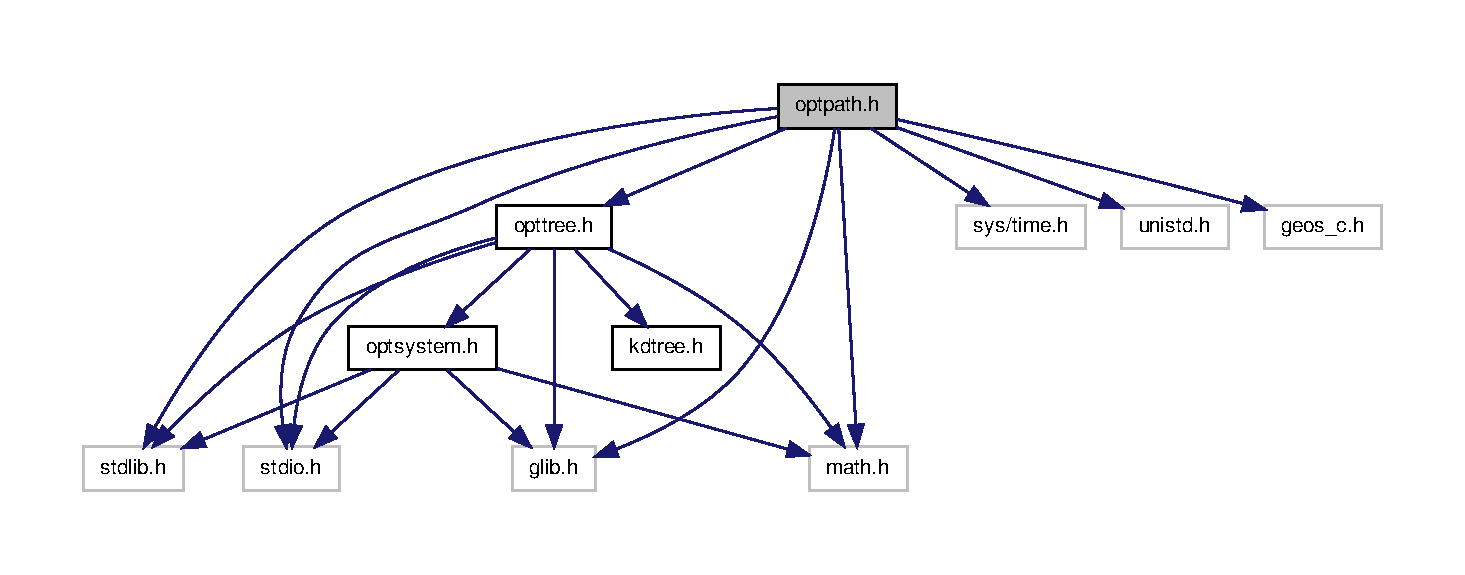
\includegraphics[width=350pt]{d6/d5b/a00026}
\end{center}
\end{figure}
\-This graph shows which files directly or indirectly include this file\-:\nopagebreak
\begin{figure}[H]
\begin{center}
\leavevmode
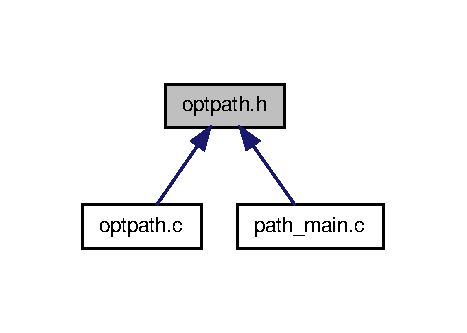
\includegraphics[width=224pt]{d0/d33/a00027}
\end{center}
\end{figure}
\subsection*{\-Defines}
\begin{DoxyCompactItemize}
\item 
\#define \hyperlink{a00016_a34379dd7ba936e396501b48e735a1b20_a34379dd7ba936e396501b48e735a1b20}{\-P\-U\-B\-L\-I\-S\-H\-\_\-\-N\-O\-D\-E\-S\-\_\-\-E\-D\-G\-E\-S}~0
\item 
\#define \hyperlink{a00016_ad85ab7068113dc84475cf30652874115_ad85ab7068113dc84475cf30652874115}{\-M\-E\-D\-\_\-\-C\-E\-N\-T\-E\-R\-\_\-\-X}~20
\item 
\#define \hyperlink{a00016_ae5ab8dd26396714a32a2a4ce7fc378f0_ae5ab8dd26396714a32a2a4ce7fc378f0}{\-M\-E\-D\-\_\-\-C\-E\-N\-T\-E\-R\-\_\-\-Y}~40
\item 
\#define \hyperlink{a00016_aab4929fd443830fa88546b2cb4e945a9_aab4929fd443830fa88546b2cb4e945a9}{\-M\-E\-D\-\_\-\-S\-I\-Z\-E\-\_\-\-X}~60
\item 
\#define \hyperlink{a00016_ac51d633b8a48950f88c946c1d175e25c_ac51d633b8a48950f88c946c1d175e25c}{\-M\-E\-D\-\_\-\-S\-I\-Z\-E\-\_\-\-Y}~20
\item 
\#define \hyperlink{a00016_a0da9666928ebcac616516774a85f7a1e_a0da9666928ebcac616516774a85f7a1e}{\-B\-A\-L\-T\-\_\-\-C\-E\-N\-T\-E\-R\-\_\-\-X}~23
\item 
\#define \hyperlink{a00016_a66530f0c393d2e538914b632edb59104_a66530f0c393d2e538914b632edb59104}{\-B\-A\-L\-T\-\_\-\-C\-E\-N\-T\-E\-R\-\_\-\-Y}~60
\item 
\#define \hyperlink{a00016_a14ccd5b0a841f759310f5d3b6208cf5a_a14ccd5b0a841f759310f5d3b6208cf5a}{\-B\-A\-L\-T\-\_\-\-S\-I\-Z\-E\-\_\-\-X}~14
\item 
\#define \hyperlink{a00016_a1c1e285f8b1a74ec8609e73b5ad4fd04_a1c1e285f8b1a74ec8609e73b5ad4fd04}{\-B\-A\-L\-T\-\_\-\-S\-I\-Z\-E\-\_\-\-Y}~12
\item 
\#define \hyperlink{a00016_adba9613a36cb7c246ce7d88c46fdb74c_adba9613a36cb7c246ce7d88c46fdb74c}{\-N\-O\-R\-T\-H\-\_\-\-C\-E\-N\-T\-E\-R\-\_\-\-X}~11
\item 
\#define \hyperlink{a00016_a09ebccefe21eeb37dbc59bb722a2e6eb_a09ebccefe21eeb37dbc59bb722a2e6eb}{\-N\-O\-R\-T\-H\-\_\-\-C\-E\-N\-T\-E\-R\-\_\-\-Y}~56.\-5
\item 
\#define \hyperlink{a00016_a9adc5f9b5d673521744d30ca4c5e42c6_a9adc5f9b5d673521744d30ca4c5e42c6}{\-N\-O\-R\-T\-H\-\_\-\-S\-I\-Z\-E\-\_\-\-X}~10
\item 
\#define \hyperlink{a00016_aeebc2f024b71e1c7e21a4aa84df6c658_aeebc2f024b71e1c7e21a4aa84df6c658}{\-N\-O\-R\-T\-H\-\_\-\-S\-I\-Z\-E\-\_\-\-Y}~7
\item 
\#define \hyperlink{a00016_aea54516d126e26f705a90f2554088aa7_aea54516d126e26f705a90f2554088aa7}{\-W\-O\-R\-L\-D\-\_\-\-C\-E\-N\-T\-E\-R\-\_\-\-X}~0
\item 
\#define \hyperlink{a00016_a2df4ec3ebf3dfb2571bad3b77c71362d_a2df4ec3ebf3dfb2571bad3b77c71362d}{\-W\-O\-R\-L\-D\-\_\-\-C\-E\-N\-T\-E\-R\-\_\-\-Y}~0
\item 
\#define \hyperlink{a00016_a0b8180d45b4f486b0376164e8d4236d4_a0b8180d45b4f486b0376164e8d4236d4}{\-W\-O\-R\-L\-D\-\_\-\-S\-I\-Z\-E\-\_\-\-X}~360
\item 
\#define \hyperlink{a00016_ace6bb03745896c34e3d7d2c6ab92cb3b_ace6bb03745896c34e3d7d2c6ab92cb3b}{\-W\-O\-R\-L\-D\-\_\-\-S\-I\-Z\-E\-\_\-\-Y}~180
\item 
\#define \hyperlink{a00016_a549d41dcf9444ed7d6df1da3c73e7d16_a549d41dcf9444ed7d6df1da3c73e7d16}{\-M\-I\-N\-\_\-\-D\-I\-S\-T\-A\-N\-C\-E}~20
\item 
\#define \hyperlink{a00016_a84b7254ec9a316504fdaffaf572f5c90_a84b7254ec9a316504fdaffaf572f5c90}{\-S\-I\-Z\-E\-\_\-\-C\-L\-O\-S\-E\-\_\-\-P\-O\-I\-N\-T}~1
\item 
\#define \hyperlink{a00016_a7abba20fa878f41f24a08abffde9b313_a7abba20fa878f41f24a08abffde9b313}{\-S\-I\-Z\-E\-\_\-\-F\-A\-R\-\_\-\-P\-O\-I\-N\-T}~4
\item 
\#define \hyperlink{a00016_aefa7672f40a44cb9b17c8fb46210d1fd_aefa7672f40a44cb9b17c8fb46210d1fd}{\-M\-A\-X\-\_\-\-I\-T\-E\-R\-A\-T\-I\-O\-N}~1000000
\item 
\#define \hyperlink{a00016_a0bfcf094f7b3bcaaa5ff91d287f07b51_a0bfcf094f7b3bcaaa5ff91d287f07b51}{\-C\-O\-M\-P\-R\-E\-S\-S\-I\-O\-N\-\_\-\-F\-A\-C\-T\-O\-R}~20
\item 
\#define \hyperlink{a00016_afd2b92c197f45f4b4f0787d4d0541c94_afd2b92c197f45f4b4f0787d4d0541c94}{\-O\-B\-S\-T\-A\-C\-L\-E\-S}~\char`\"{}obstacles.\-geojson\char`\"{}
\item 
\#define \hyperlink{a00016_a5b5cba0b0b9b73eb1ce8afda91fe7be7_a5b5cba0b0b9b73eb1ce8afda91fe7be7}{\-R\-O\-U\-T\-E}~\char`\"{}planisphere.\-geojson\char`\"{}
\item 
\#define \hyperlink{a00016_ab4bf926a45354a2f328f1a7b94ebd3c5_ab4bf926a45354a2f328f1a7b94ebd3c5}{\-D\-I\-S\-P\-L\-A\-Y}~1
\item 
\#define \hyperlink{a00016_abd5b73b8937670d0c501932fb4497d02_abd5b73b8937670d0c501932fb4497d02}{point\-\_\-see}(x, y)~do \{if (\hyperlink{a00016_ab4bf926a45354a2f328f1a7b94ebd3c5_ab4bf926a45354a2f328f1a7b94ebd3c5}{\-D\-I\-S\-P\-L\-A\-Y}) printf(\char`\"{}\%lf,\%lf$\backslash$n\char`\"{},x,y);\} while(0)
\item 
\#define \hyperlink{a00016_a697acf769962bc23eb3413977c54c639_a697acf769962bc23eb3413977c54c639}{error}(x)~do \{if (\hyperlink{a00016_ab4bf926a45354a2f328f1a7b94ebd3c5_ab4bf926a45354a2f328f1a7b94ebd3c5}{\-D\-I\-S\-P\-L\-A\-Y}) printf(\char`\"{}\-E\-R\-R\-O\-R\-: \%s\char`\"{}, x);\} while(0)
\item 
\#define \hyperlink{a00016_a84f6fe04dcb629e501acaa6a238c9a02_a84f6fe04dcb629e501acaa6a238c9a02}{time\-\_\-cost}(x, y)~do \{if (\hyperlink{a00016_ab4bf926a45354a2f328f1a7b94ebd3c5_ab4bf926a45354a2f328f1a7b94ebd3c5}{\-D\-I\-S\-P\-L\-A\-Y}) \{ printf(\char`\"{}\-Time\-: \%5.\-5lf, Cost\-: \%5.\-5lf$\backslash$n\char`\"{},x,y); \}\} while(0)
\item 
\#define \hyperlink{a00016_adbf07a45e036d82a4c5071fdd8405458_adbf07a45e036d82a4c5071fdd8405458}{warning}(x)~do \{if (\hyperlink{a00016_ab4bf926a45354a2f328f1a7b94ebd3c5_ab4bf926a45354a2f328f1a7b94ebd3c5}{\-D\-I\-S\-P\-L\-A\-Y}) \{printf(\char`\"{}number of iterations\-: \%d$\backslash$n$\backslash$n\char`\"{}, x);\}\} while(0)
\item 
\#define \hyperlink{a00016_ad31b62fe2ef557aebcf2300a672d7e36_ad31b62fe2ef557aebcf2300a672d7e36}{time\-\_\-see}(x)~do \{if (\hyperlink{a00016_ab4bf926a45354a2f328f1a7b94ebd3c5_ab4bf926a45354a2f328f1a7b94ebd3c5}{\-D\-I\-S\-P\-L\-A\-Y}) printf(\char`\"{}\%5.\-5lf$\backslash$n\char`\"{},x);\} while(0)
\end{DoxyCompactItemize}
\subsection*{\-Enumerations}
\begin{DoxyCompactItemize}
\item 
enum \hyperlink{a00016_a5f269c22e6d9d32b0b0ad7e6166854df_a5f269c22e6d9d32b0b0ad7e6166854df}{location} \{ \*
\hyperlink{a00016_a5f269c22e6d9d32b0b0ad7e6166854df_a5f269c22e6d9d32b0b0ad7e6166854dfa235f8123c86ea3fc40e1b6cd1ed7c172}{\-B\-L\-A\-C\-K\-\_\-\-S\-E\-A}, 
\hyperlink{a00016_a5f269c22e6d9d32b0b0ad7e6166854df_a5f269c22e6d9d32b0b0ad7e6166854dfa9c3327b166a4167a933b7c8f1e15583b}{\-M\-E\-D\-E\-T\-E\-R\-A\-N\-I\-A\-N}, 
\hyperlink{a00016_a5f269c22e6d9d32b0b0ad7e6166854df_a5f269c22e6d9d32b0b0ad7e6166854dfa6dedb45f6c3ac5daec9bb907224206dc}{\-B\-A\-L\-T\-I\-C\-\_\-\-S\-E\-A}, 
\hyperlink{a00016_a5f269c22e6d9d32b0b0ad7e6166854df_a5f269c22e6d9d32b0b0ad7e6166854dfaad03d1c98aa862f00130d0d17a96b9e6}{\-N\-O\-R\-T\-H\-\_\-\-S\-E\-A}, 
\*
\hyperlink{a00016_a5f269c22e6d9d32b0b0ad7e6166854df_a5f269c22e6d9d32b0b0ad7e6166854dfa8124d17f836efbb680ba3311e78c8cba}{\-O\-R\-D\-I\-N\-A\-R\-Y}
 \}
\begin{DoxyCompactList}\small\item\em \-Location of a point. \end{DoxyCompactList}\end{DoxyCompactItemize}
\subsection*{\-Functions}
\begin{DoxyCompactItemize}
\item 
void \hyperlink{a00016_abb72a9e5586947ffa14de7aea6c8d7b4_abb72a9e5586947ffa14de7aea6c8d7b4}{notice1} (const char $\ast$fmt,...)
\item 
void \hyperlink{a00016_ab369473e6f056b28d426c97004c47828_ab369473e6f056b28d426c97004c47828}{log\-\_\-and\-\_\-exit1} (const char $\ast$fmt,...)
\item 
\-G\-S\-List $\ast$ \hyperlink{a00016_a5fbe870a8fdafd7aedaf1591ffb214a9_a5fbe870a8fdafd7aedaf1591ffb214a9}{path} (double x\-\_\-root, double y\-\_\-root, double x\-\_\-arrival, double y\-\_\-arrival, char $\ast$obstacle)
\begin{DoxyCompactList}\small\item\em \-This function calculate the shortest path between two points\-: applicate rrtstar alogorithm, then use the correcting path algorithm to affinate the result. \end{DoxyCompactList}\item 
\-G\-S\-List $\ast$ \hyperlink{a00016_afd836348eeb1fd77cd7967c9ba1a08fb_afd836348eeb1fd77cd7967c9ba1a08fb}{final\-\_\-path} (double x\-\_\-root, double y\-\_\-root, double x\-\_\-arrival, double y\-\_\-arrival, char $\ast$obstacles)
\begin{DoxyCompactList}\small\item\em \-This function calculate the final path that could be a connexion between 2 paths, then it fill the geojson file of the trajectory. \end{DoxyCompactList}\item 
\hyperlink{a00016_a5f269c22e6d9d32b0b0ad7e6166854df_a5f269c22e6d9d32b0b0ad7e6166854df}{location} \hyperlink{a00016_a8fccd24d5b565d686f8ffd2820bf372a_a8fccd24d5b565d686f8ffd2820bf372a}{locat\-\_\-point} (double x, double y)
\begin{DoxyCompactList}\small\item\em find the location of a given point \end{DoxyCompactList}\item 
\hyperlink{a00020_a07b75293fafb6f31b7e9f723848ad105_a07b75293fafb6f31b7e9f723848ad105}{opttree\-\_\-t} $\ast$ \hyperlink{a00016_ad57de17f688b7fd9ae8db3dee4c728a3_ad57de17f688b7fd9ae8db3dee4c728a3}{create\-\_\-environnement} (double x\-\_\-root, double y\-\_\-root, double x\-\_\-arrival, double y\-\_\-arrival, char $\ast$obstacle, int k)
\begin{DoxyCompactList}\small\item\em create the work environement; actually root\-\_\-state, goal\-\_\-region, operating region(depending on departure and arrival) and obstacle list(continents) \end{DoxyCompactList}\item 
\-G\-S\-List $\ast$ \hyperlink{a00016_ace68cd1543a0636ed5bbd81dde6e294f_ace68cd1543a0636ed5bbd81dde6e294f}{dividing\-\_\-path} (double x1, double y1, double x2, double y2, char $\ast$obstacle, \hyperlink{a00016_a5f269c22e6d9d32b0b0ad7e6166854df_a5f269c22e6d9d32b0b0ad7e6166854df}{location} loc)
\begin{DoxyCompactList}\small\item\em \-This function is used when one of the daparture or arrival point is situated in one of the complex area already defined. \end{DoxyCompactList}\item 
\-G\-S\-List $\ast$ \hyperlink{a00016_a2a7bcf30e2fa1f22726a7c5187fd7aea_a2a7bcf30e2fa1f22726a7c5187fd7aea}{correcting\-\_\-path} (\hyperlink{a00020_a07b75293fafb6f31b7e9f723848ad105_a07b75293fafb6f31b7e9f723848ad105}{opttree\-\_\-t} $\ast$opttree, \-G\-S\-List $\ast$optstates\-\_\-list, int k)
\begin{DoxyCompactList}\small\item\em from a path between two points (the result of rrtstar algorithm but with minimum number of iterations), make a better one by eleminating nodes and adding others \end{DoxyCompactList}\end{DoxyCompactItemize}


\subsection{\-Define \-Documentation}
\hypertarget{a00016_a0da9666928ebcac616516774a85f7a1e_a0da9666928ebcac616516774a85f7a1e}{\index{optpath.\-h@{optpath.\-h}!\-B\-A\-L\-T\-\_\-\-C\-E\-N\-T\-E\-R\-\_\-\-X@{\-B\-A\-L\-T\-\_\-\-C\-E\-N\-T\-E\-R\-\_\-\-X}}
\index{\-B\-A\-L\-T\-\_\-\-C\-E\-N\-T\-E\-R\-\_\-\-X@{\-B\-A\-L\-T\-\_\-\-C\-E\-N\-T\-E\-R\-\_\-\-X}!optpath.h@{optpath.\-h}}
\subsubsection[{\-B\-A\-L\-T\-\_\-\-C\-E\-N\-T\-E\-R\-\_\-\-X}]{\setlength{\rightskip}{0pt plus 5cm}\#define {\bf \-B\-A\-L\-T\-\_\-\-C\-E\-N\-T\-E\-R\-\_\-\-X}~23}}\label{d7/d7a/a00016_a0da9666928ebcac616516774a85f7a1e_a0da9666928ebcac616516774a85f7a1e}
\hypertarget{a00016_a66530f0c393d2e538914b632edb59104_a66530f0c393d2e538914b632edb59104}{\index{optpath.\-h@{optpath.\-h}!\-B\-A\-L\-T\-\_\-\-C\-E\-N\-T\-E\-R\-\_\-\-Y@{\-B\-A\-L\-T\-\_\-\-C\-E\-N\-T\-E\-R\-\_\-\-Y}}
\index{\-B\-A\-L\-T\-\_\-\-C\-E\-N\-T\-E\-R\-\_\-\-Y@{\-B\-A\-L\-T\-\_\-\-C\-E\-N\-T\-E\-R\-\_\-\-Y}!optpath.h@{optpath.\-h}}
\subsubsection[{\-B\-A\-L\-T\-\_\-\-C\-E\-N\-T\-E\-R\-\_\-\-Y}]{\setlength{\rightskip}{0pt plus 5cm}\#define {\bf \-B\-A\-L\-T\-\_\-\-C\-E\-N\-T\-E\-R\-\_\-\-Y}~60}}\label{d7/d7a/a00016_a66530f0c393d2e538914b632edb59104_a66530f0c393d2e538914b632edb59104}
\hypertarget{a00016_a14ccd5b0a841f759310f5d3b6208cf5a_a14ccd5b0a841f759310f5d3b6208cf5a}{\index{optpath.\-h@{optpath.\-h}!\-B\-A\-L\-T\-\_\-\-S\-I\-Z\-E\-\_\-\-X@{\-B\-A\-L\-T\-\_\-\-S\-I\-Z\-E\-\_\-\-X}}
\index{\-B\-A\-L\-T\-\_\-\-S\-I\-Z\-E\-\_\-\-X@{\-B\-A\-L\-T\-\_\-\-S\-I\-Z\-E\-\_\-\-X}!optpath.h@{optpath.\-h}}
\subsubsection[{\-B\-A\-L\-T\-\_\-\-S\-I\-Z\-E\-\_\-\-X}]{\setlength{\rightskip}{0pt plus 5cm}\#define {\bf \-B\-A\-L\-T\-\_\-\-S\-I\-Z\-E\-\_\-\-X}~14}}\label{d7/d7a/a00016_a14ccd5b0a841f759310f5d3b6208cf5a_a14ccd5b0a841f759310f5d3b6208cf5a}
\hypertarget{a00016_a1c1e285f8b1a74ec8609e73b5ad4fd04_a1c1e285f8b1a74ec8609e73b5ad4fd04}{\index{optpath.\-h@{optpath.\-h}!\-B\-A\-L\-T\-\_\-\-S\-I\-Z\-E\-\_\-\-Y@{\-B\-A\-L\-T\-\_\-\-S\-I\-Z\-E\-\_\-\-Y}}
\index{\-B\-A\-L\-T\-\_\-\-S\-I\-Z\-E\-\_\-\-Y@{\-B\-A\-L\-T\-\_\-\-S\-I\-Z\-E\-\_\-\-Y}!optpath.h@{optpath.\-h}}
\subsubsection[{\-B\-A\-L\-T\-\_\-\-S\-I\-Z\-E\-\_\-\-Y}]{\setlength{\rightskip}{0pt plus 5cm}\#define {\bf \-B\-A\-L\-T\-\_\-\-S\-I\-Z\-E\-\_\-\-Y}~12}}\label{d7/d7a/a00016_a1c1e285f8b1a74ec8609e73b5ad4fd04_a1c1e285f8b1a74ec8609e73b5ad4fd04}
\hypertarget{a00016_a0bfcf094f7b3bcaaa5ff91d287f07b51_a0bfcf094f7b3bcaaa5ff91d287f07b51}{\index{optpath.\-h@{optpath.\-h}!\-C\-O\-M\-P\-R\-E\-S\-S\-I\-O\-N\-\_\-\-F\-A\-C\-T\-O\-R@{\-C\-O\-M\-P\-R\-E\-S\-S\-I\-O\-N\-\_\-\-F\-A\-C\-T\-O\-R}}
\index{\-C\-O\-M\-P\-R\-E\-S\-S\-I\-O\-N\-\_\-\-F\-A\-C\-T\-O\-R@{\-C\-O\-M\-P\-R\-E\-S\-S\-I\-O\-N\-\_\-\-F\-A\-C\-T\-O\-R}!optpath.h@{optpath.\-h}}
\subsubsection[{\-C\-O\-M\-P\-R\-E\-S\-S\-I\-O\-N\-\_\-\-F\-A\-C\-T\-O\-R}]{\setlength{\rightskip}{0pt plus 5cm}\#define {\bf \-C\-O\-M\-P\-R\-E\-S\-S\-I\-O\-N\-\_\-\-F\-A\-C\-T\-O\-R}~20}}\label{d7/d7a/a00016_a0bfcf094f7b3bcaaa5ff91d287f07b51_a0bfcf094f7b3bcaaa5ff91d287f07b51}
\hypertarget{a00016_ab4bf926a45354a2f328f1a7b94ebd3c5_ab4bf926a45354a2f328f1a7b94ebd3c5}{\index{optpath.\-h@{optpath.\-h}!\-D\-I\-S\-P\-L\-A\-Y@{\-D\-I\-S\-P\-L\-A\-Y}}
\index{\-D\-I\-S\-P\-L\-A\-Y@{\-D\-I\-S\-P\-L\-A\-Y}!optpath.h@{optpath.\-h}}
\subsubsection[{\-D\-I\-S\-P\-L\-A\-Y}]{\setlength{\rightskip}{0pt plus 5cm}\#define {\bf \-D\-I\-S\-P\-L\-A\-Y}~1}}\label{d7/d7a/a00016_ab4bf926a45354a2f328f1a7b94ebd3c5_ab4bf926a45354a2f328f1a7b94ebd3c5}
\hypertarget{a00016_a697acf769962bc23eb3413977c54c639_a697acf769962bc23eb3413977c54c639}{\index{optpath.\-h@{optpath.\-h}!error@{error}}
\index{error@{error}!optpath.h@{optpath.\-h}}
\subsubsection[{error}]{\setlength{\rightskip}{0pt plus 5cm}\#define {\bf error}(
\begin{DoxyParamCaption}
\item[{}]{x}
\end{DoxyParamCaption}
)~do \{if ({\bf \-D\-I\-S\-P\-L\-A\-Y}) printf(\char`\"{}\-E\-R\-R\-O\-R\-: \%s\char`\"{}, x);\} while(0)}}\label{d7/d7a/a00016_a697acf769962bc23eb3413977c54c639_a697acf769962bc23eb3413977c54c639}
\hypertarget{a00016_aefa7672f40a44cb9b17c8fb46210d1fd_aefa7672f40a44cb9b17c8fb46210d1fd}{\index{optpath.\-h@{optpath.\-h}!\-M\-A\-X\-\_\-\-I\-T\-E\-R\-A\-T\-I\-O\-N@{\-M\-A\-X\-\_\-\-I\-T\-E\-R\-A\-T\-I\-O\-N}}
\index{\-M\-A\-X\-\_\-\-I\-T\-E\-R\-A\-T\-I\-O\-N@{\-M\-A\-X\-\_\-\-I\-T\-E\-R\-A\-T\-I\-O\-N}!optpath.h@{optpath.\-h}}
\subsubsection[{\-M\-A\-X\-\_\-\-I\-T\-E\-R\-A\-T\-I\-O\-N}]{\setlength{\rightskip}{0pt plus 5cm}\#define {\bf \-M\-A\-X\-\_\-\-I\-T\-E\-R\-A\-T\-I\-O\-N}~1000000}}\label{d7/d7a/a00016_aefa7672f40a44cb9b17c8fb46210d1fd_aefa7672f40a44cb9b17c8fb46210d1fd}
\hypertarget{a00016_ad85ab7068113dc84475cf30652874115_ad85ab7068113dc84475cf30652874115}{\index{optpath.\-h@{optpath.\-h}!\-M\-E\-D\-\_\-\-C\-E\-N\-T\-E\-R\-\_\-\-X@{\-M\-E\-D\-\_\-\-C\-E\-N\-T\-E\-R\-\_\-\-X}}
\index{\-M\-E\-D\-\_\-\-C\-E\-N\-T\-E\-R\-\_\-\-X@{\-M\-E\-D\-\_\-\-C\-E\-N\-T\-E\-R\-\_\-\-X}!optpath.h@{optpath.\-h}}
\subsubsection[{\-M\-E\-D\-\_\-\-C\-E\-N\-T\-E\-R\-\_\-\-X}]{\setlength{\rightskip}{0pt plus 5cm}\#define {\bf \-M\-E\-D\-\_\-\-C\-E\-N\-T\-E\-R\-\_\-\-X}~20}}\label{d7/d7a/a00016_ad85ab7068113dc84475cf30652874115_ad85ab7068113dc84475cf30652874115}
\hypertarget{a00016_ae5ab8dd26396714a32a2a4ce7fc378f0_ae5ab8dd26396714a32a2a4ce7fc378f0}{\index{optpath.\-h@{optpath.\-h}!\-M\-E\-D\-\_\-\-C\-E\-N\-T\-E\-R\-\_\-\-Y@{\-M\-E\-D\-\_\-\-C\-E\-N\-T\-E\-R\-\_\-\-Y}}
\index{\-M\-E\-D\-\_\-\-C\-E\-N\-T\-E\-R\-\_\-\-Y@{\-M\-E\-D\-\_\-\-C\-E\-N\-T\-E\-R\-\_\-\-Y}!optpath.h@{optpath.\-h}}
\subsubsection[{\-M\-E\-D\-\_\-\-C\-E\-N\-T\-E\-R\-\_\-\-Y}]{\setlength{\rightskip}{0pt plus 5cm}\#define {\bf \-M\-E\-D\-\_\-\-C\-E\-N\-T\-E\-R\-\_\-\-Y}~40}}\label{d7/d7a/a00016_ae5ab8dd26396714a32a2a4ce7fc378f0_ae5ab8dd26396714a32a2a4ce7fc378f0}
\hypertarget{a00016_aab4929fd443830fa88546b2cb4e945a9_aab4929fd443830fa88546b2cb4e945a9}{\index{optpath.\-h@{optpath.\-h}!\-M\-E\-D\-\_\-\-S\-I\-Z\-E\-\_\-\-X@{\-M\-E\-D\-\_\-\-S\-I\-Z\-E\-\_\-\-X}}
\index{\-M\-E\-D\-\_\-\-S\-I\-Z\-E\-\_\-\-X@{\-M\-E\-D\-\_\-\-S\-I\-Z\-E\-\_\-\-X}!optpath.h@{optpath.\-h}}
\subsubsection[{\-M\-E\-D\-\_\-\-S\-I\-Z\-E\-\_\-\-X}]{\setlength{\rightskip}{0pt plus 5cm}\#define {\bf \-M\-E\-D\-\_\-\-S\-I\-Z\-E\-\_\-\-X}~60}}\label{d7/d7a/a00016_aab4929fd443830fa88546b2cb4e945a9_aab4929fd443830fa88546b2cb4e945a9}
\hypertarget{a00016_ac51d633b8a48950f88c946c1d175e25c_ac51d633b8a48950f88c946c1d175e25c}{\index{optpath.\-h@{optpath.\-h}!\-M\-E\-D\-\_\-\-S\-I\-Z\-E\-\_\-\-Y@{\-M\-E\-D\-\_\-\-S\-I\-Z\-E\-\_\-\-Y}}
\index{\-M\-E\-D\-\_\-\-S\-I\-Z\-E\-\_\-\-Y@{\-M\-E\-D\-\_\-\-S\-I\-Z\-E\-\_\-\-Y}!optpath.h@{optpath.\-h}}
\subsubsection[{\-M\-E\-D\-\_\-\-S\-I\-Z\-E\-\_\-\-Y}]{\setlength{\rightskip}{0pt plus 5cm}\#define {\bf \-M\-E\-D\-\_\-\-S\-I\-Z\-E\-\_\-\-Y}~20}}\label{d7/d7a/a00016_ac51d633b8a48950f88c946c1d175e25c_ac51d633b8a48950f88c946c1d175e25c}
\hypertarget{a00016_a549d41dcf9444ed7d6df1da3c73e7d16_a549d41dcf9444ed7d6df1da3c73e7d16}{\index{optpath.\-h@{optpath.\-h}!\-M\-I\-N\-\_\-\-D\-I\-S\-T\-A\-N\-C\-E@{\-M\-I\-N\-\_\-\-D\-I\-S\-T\-A\-N\-C\-E}}
\index{\-M\-I\-N\-\_\-\-D\-I\-S\-T\-A\-N\-C\-E@{\-M\-I\-N\-\_\-\-D\-I\-S\-T\-A\-N\-C\-E}!optpath.h@{optpath.\-h}}
\subsubsection[{\-M\-I\-N\-\_\-\-D\-I\-S\-T\-A\-N\-C\-E}]{\setlength{\rightskip}{0pt plus 5cm}\#define {\bf \-M\-I\-N\-\_\-\-D\-I\-S\-T\-A\-N\-C\-E}~20}}\label{d7/d7a/a00016_a549d41dcf9444ed7d6df1da3c73e7d16_a549d41dcf9444ed7d6df1da3c73e7d16}
\hypertarget{a00016_adba9613a36cb7c246ce7d88c46fdb74c_adba9613a36cb7c246ce7d88c46fdb74c}{\index{optpath.\-h@{optpath.\-h}!\-N\-O\-R\-T\-H\-\_\-\-C\-E\-N\-T\-E\-R\-\_\-\-X@{\-N\-O\-R\-T\-H\-\_\-\-C\-E\-N\-T\-E\-R\-\_\-\-X}}
\index{\-N\-O\-R\-T\-H\-\_\-\-C\-E\-N\-T\-E\-R\-\_\-\-X@{\-N\-O\-R\-T\-H\-\_\-\-C\-E\-N\-T\-E\-R\-\_\-\-X}!optpath.h@{optpath.\-h}}
\subsubsection[{\-N\-O\-R\-T\-H\-\_\-\-C\-E\-N\-T\-E\-R\-\_\-\-X}]{\setlength{\rightskip}{0pt plus 5cm}\#define {\bf \-N\-O\-R\-T\-H\-\_\-\-C\-E\-N\-T\-E\-R\-\_\-\-X}~11}}\label{d7/d7a/a00016_adba9613a36cb7c246ce7d88c46fdb74c_adba9613a36cb7c246ce7d88c46fdb74c}
\hypertarget{a00016_a09ebccefe21eeb37dbc59bb722a2e6eb_a09ebccefe21eeb37dbc59bb722a2e6eb}{\index{optpath.\-h@{optpath.\-h}!\-N\-O\-R\-T\-H\-\_\-\-C\-E\-N\-T\-E\-R\-\_\-\-Y@{\-N\-O\-R\-T\-H\-\_\-\-C\-E\-N\-T\-E\-R\-\_\-\-Y}}
\index{\-N\-O\-R\-T\-H\-\_\-\-C\-E\-N\-T\-E\-R\-\_\-\-Y@{\-N\-O\-R\-T\-H\-\_\-\-C\-E\-N\-T\-E\-R\-\_\-\-Y}!optpath.h@{optpath.\-h}}
\subsubsection[{\-N\-O\-R\-T\-H\-\_\-\-C\-E\-N\-T\-E\-R\-\_\-\-Y}]{\setlength{\rightskip}{0pt plus 5cm}\#define {\bf \-N\-O\-R\-T\-H\-\_\-\-C\-E\-N\-T\-E\-R\-\_\-\-Y}~56.\-5}}\label{d7/d7a/a00016_a09ebccefe21eeb37dbc59bb722a2e6eb_a09ebccefe21eeb37dbc59bb722a2e6eb}
\hypertarget{a00016_a9adc5f9b5d673521744d30ca4c5e42c6_a9adc5f9b5d673521744d30ca4c5e42c6}{\index{optpath.\-h@{optpath.\-h}!\-N\-O\-R\-T\-H\-\_\-\-S\-I\-Z\-E\-\_\-\-X@{\-N\-O\-R\-T\-H\-\_\-\-S\-I\-Z\-E\-\_\-\-X}}
\index{\-N\-O\-R\-T\-H\-\_\-\-S\-I\-Z\-E\-\_\-\-X@{\-N\-O\-R\-T\-H\-\_\-\-S\-I\-Z\-E\-\_\-\-X}!optpath.h@{optpath.\-h}}
\subsubsection[{\-N\-O\-R\-T\-H\-\_\-\-S\-I\-Z\-E\-\_\-\-X}]{\setlength{\rightskip}{0pt plus 5cm}\#define {\bf \-N\-O\-R\-T\-H\-\_\-\-S\-I\-Z\-E\-\_\-\-X}~10}}\label{d7/d7a/a00016_a9adc5f9b5d673521744d30ca4c5e42c6_a9adc5f9b5d673521744d30ca4c5e42c6}
\hypertarget{a00016_aeebc2f024b71e1c7e21a4aa84df6c658_aeebc2f024b71e1c7e21a4aa84df6c658}{\index{optpath.\-h@{optpath.\-h}!\-N\-O\-R\-T\-H\-\_\-\-S\-I\-Z\-E\-\_\-\-Y@{\-N\-O\-R\-T\-H\-\_\-\-S\-I\-Z\-E\-\_\-\-Y}}
\index{\-N\-O\-R\-T\-H\-\_\-\-S\-I\-Z\-E\-\_\-\-Y@{\-N\-O\-R\-T\-H\-\_\-\-S\-I\-Z\-E\-\_\-\-Y}!optpath.h@{optpath.\-h}}
\subsubsection[{\-N\-O\-R\-T\-H\-\_\-\-S\-I\-Z\-E\-\_\-\-Y}]{\setlength{\rightskip}{0pt plus 5cm}\#define {\bf \-N\-O\-R\-T\-H\-\_\-\-S\-I\-Z\-E\-\_\-\-Y}~7}}\label{d7/d7a/a00016_aeebc2f024b71e1c7e21a4aa84df6c658_aeebc2f024b71e1c7e21a4aa84df6c658}
\hypertarget{a00016_afd2b92c197f45f4b4f0787d4d0541c94_afd2b92c197f45f4b4f0787d4d0541c94}{\index{optpath.\-h@{optpath.\-h}!\-O\-B\-S\-T\-A\-C\-L\-E\-S@{\-O\-B\-S\-T\-A\-C\-L\-E\-S}}
\index{\-O\-B\-S\-T\-A\-C\-L\-E\-S@{\-O\-B\-S\-T\-A\-C\-L\-E\-S}!optpath.h@{optpath.\-h}}
\subsubsection[{\-O\-B\-S\-T\-A\-C\-L\-E\-S}]{\setlength{\rightskip}{0pt plus 5cm}\#define {\bf \-O\-B\-S\-T\-A\-C\-L\-E\-S}~\char`\"{}obstacles.\-geojson\char`\"{}}}\label{d7/d7a/a00016_afd2b92c197f45f4b4f0787d4d0541c94_afd2b92c197f45f4b4f0787d4d0541c94}
\hypertarget{a00016_abd5b73b8937670d0c501932fb4497d02_abd5b73b8937670d0c501932fb4497d02}{\index{optpath.\-h@{optpath.\-h}!point\-\_\-see@{point\-\_\-see}}
\index{point\-\_\-see@{point\-\_\-see}!optpath.h@{optpath.\-h}}
\subsubsection[{point\-\_\-see}]{\setlength{\rightskip}{0pt plus 5cm}\#define {\bf point\-\_\-see}(
\begin{DoxyParamCaption}
\item[{}]{x, }
\item[{}]{y}
\end{DoxyParamCaption}
)~do \{if ({\bf \-D\-I\-S\-P\-L\-A\-Y}) printf(\char`\"{}\%lf,\%lf$\backslash$n\char`\"{},x,y);\} while(0)}}\label{d7/d7a/a00016_abd5b73b8937670d0c501932fb4497d02_abd5b73b8937670d0c501932fb4497d02}
\hypertarget{a00016_a34379dd7ba936e396501b48e735a1b20_a34379dd7ba936e396501b48e735a1b20}{\index{optpath.\-h@{optpath.\-h}!\-P\-U\-B\-L\-I\-S\-H\-\_\-\-N\-O\-D\-E\-S\-\_\-\-E\-D\-G\-E\-S@{\-P\-U\-B\-L\-I\-S\-H\-\_\-\-N\-O\-D\-E\-S\-\_\-\-E\-D\-G\-E\-S}}
\index{\-P\-U\-B\-L\-I\-S\-H\-\_\-\-N\-O\-D\-E\-S\-\_\-\-E\-D\-G\-E\-S@{\-P\-U\-B\-L\-I\-S\-H\-\_\-\-N\-O\-D\-E\-S\-\_\-\-E\-D\-G\-E\-S}!optpath.h@{optpath.\-h}}
\subsubsection[{\-P\-U\-B\-L\-I\-S\-H\-\_\-\-N\-O\-D\-E\-S\-\_\-\-E\-D\-G\-E\-S}]{\setlength{\rightskip}{0pt plus 5cm}\#define {\bf \-P\-U\-B\-L\-I\-S\-H\-\_\-\-N\-O\-D\-E\-S\-\_\-\-E\-D\-G\-E\-S}~0}}\label{d7/d7a/a00016_a34379dd7ba936e396501b48e735a1b20_a34379dd7ba936e396501b48e735a1b20}
\hypertarget{a00016_a5b5cba0b0b9b73eb1ce8afda91fe7be7_a5b5cba0b0b9b73eb1ce8afda91fe7be7}{\index{optpath.\-h@{optpath.\-h}!\-R\-O\-U\-T\-E@{\-R\-O\-U\-T\-E}}
\index{\-R\-O\-U\-T\-E@{\-R\-O\-U\-T\-E}!optpath.h@{optpath.\-h}}
\subsubsection[{\-R\-O\-U\-T\-E}]{\setlength{\rightskip}{0pt plus 5cm}\#define {\bf \-R\-O\-U\-T\-E}~\char`\"{}planisphere.\-geojson\char`\"{}}}\label{d7/d7a/a00016_a5b5cba0b0b9b73eb1ce8afda91fe7be7_a5b5cba0b0b9b73eb1ce8afda91fe7be7}
\hypertarget{a00016_a84b7254ec9a316504fdaffaf572f5c90_a84b7254ec9a316504fdaffaf572f5c90}{\index{optpath.\-h@{optpath.\-h}!\-S\-I\-Z\-E\-\_\-\-C\-L\-O\-S\-E\-\_\-\-P\-O\-I\-N\-T@{\-S\-I\-Z\-E\-\_\-\-C\-L\-O\-S\-E\-\_\-\-P\-O\-I\-N\-T}}
\index{\-S\-I\-Z\-E\-\_\-\-C\-L\-O\-S\-E\-\_\-\-P\-O\-I\-N\-T@{\-S\-I\-Z\-E\-\_\-\-C\-L\-O\-S\-E\-\_\-\-P\-O\-I\-N\-T}!optpath.h@{optpath.\-h}}
\subsubsection[{\-S\-I\-Z\-E\-\_\-\-C\-L\-O\-S\-E\-\_\-\-P\-O\-I\-N\-T}]{\setlength{\rightskip}{0pt plus 5cm}\#define {\bf \-S\-I\-Z\-E\-\_\-\-C\-L\-O\-S\-E\-\_\-\-P\-O\-I\-N\-T}~1}}\label{d7/d7a/a00016_a84b7254ec9a316504fdaffaf572f5c90_a84b7254ec9a316504fdaffaf572f5c90}
\hypertarget{a00016_a7abba20fa878f41f24a08abffde9b313_a7abba20fa878f41f24a08abffde9b313}{\index{optpath.\-h@{optpath.\-h}!\-S\-I\-Z\-E\-\_\-\-F\-A\-R\-\_\-\-P\-O\-I\-N\-T@{\-S\-I\-Z\-E\-\_\-\-F\-A\-R\-\_\-\-P\-O\-I\-N\-T}}
\index{\-S\-I\-Z\-E\-\_\-\-F\-A\-R\-\_\-\-P\-O\-I\-N\-T@{\-S\-I\-Z\-E\-\_\-\-F\-A\-R\-\_\-\-P\-O\-I\-N\-T}!optpath.h@{optpath.\-h}}
\subsubsection[{\-S\-I\-Z\-E\-\_\-\-F\-A\-R\-\_\-\-P\-O\-I\-N\-T}]{\setlength{\rightskip}{0pt plus 5cm}\#define {\bf \-S\-I\-Z\-E\-\_\-\-F\-A\-R\-\_\-\-P\-O\-I\-N\-T}~4}}\label{d7/d7a/a00016_a7abba20fa878f41f24a08abffde9b313_a7abba20fa878f41f24a08abffde9b313}
\hypertarget{a00016_a84f6fe04dcb629e501acaa6a238c9a02_a84f6fe04dcb629e501acaa6a238c9a02}{\index{optpath.\-h@{optpath.\-h}!time\-\_\-cost@{time\-\_\-cost}}
\index{time\-\_\-cost@{time\-\_\-cost}!optpath.h@{optpath.\-h}}
\subsubsection[{time\-\_\-cost}]{\setlength{\rightskip}{0pt plus 5cm}\#define {\bf time\-\_\-cost}(
\begin{DoxyParamCaption}
\item[{}]{x, }
\item[{}]{y}
\end{DoxyParamCaption}
)~do \{if ({\bf \-D\-I\-S\-P\-L\-A\-Y}) \{ printf(\char`\"{}\-Time\-: \%5.\-5lf, Cost\-: \%5.\-5lf$\backslash$n\char`\"{},x,y); \}\} while(0)}}\label{d7/d7a/a00016_a84f6fe04dcb629e501acaa6a238c9a02_a84f6fe04dcb629e501acaa6a238c9a02}
\hypertarget{a00016_ad31b62fe2ef557aebcf2300a672d7e36_ad31b62fe2ef557aebcf2300a672d7e36}{\index{optpath.\-h@{optpath.\-h}!time\-\_\-see@{time\-\_\-see}}
\index{time\-\_\-see@{time\-\_\-see}!optpath.h@{optpath.\-h}}
\subsubsection[{time\-\_\-see}]{\setlength{\rightskip}{0pt plus 5cm}\#define {\bf time\-\_\-see}(
\begin{DoxyParamCaption}
\item[{}]{x}
\end{DoxyParamCaption}
)~do \{if ({\bf \-D\-I\-S\-P\-L\-A\-Y}) printf(\char`\"{}\%5.\-5lf$\backslash$n\char`\"{},x);\} while(0)}}\label{d7/d7a/a00016_ad31b62fe2ef557aebcf2300a672d7e36_ad31b62fe2ef557aebcf2300a672d7e36}
\hypertarget{a00016_adbf07a45e036d82a4c5071fdd8405458_adbf07a45e036d82a4c5071fdd8405458}{\index{optpath.\-h@{optpath.\-h}!warning@{warning}}
\index{warning@{warning}!optpath.h@{optpath.\-h}}
\subsubsection[{warning}]{\setlength{\rightskip}{0pt plus 5cm}\#define {\bf warning}(
\begin{DoxyParamCaption}
\item[{}]{x}
\end{DoxyParamCaption}
)~do \{if ({\bf \-D\-I\-S\-P\-L\-A\-Y}) \{printf(\char`\"{}number of iterations\-: \%d$\backslash$n$\backslash$n\char`\"{}, x);\}\} while(0)}}\label{d7/d7a/a00016_adbf07a45e036d82a4c5071fdd8405458_adbf07a45e036d82a4c5071fdd8405458}
\hypertarget{a00016_aea54516d126e26f705a90f2554088aa7_aea54516d126e26f705a90f2554088aa7}{\index{optpath.\-h@{optpath.\-h}!\-W\-O\-R\-L\-D\-\_\-\-C\-E\-N\-T\-E\-R\-\_\-\-X@{\-W\-O\-R\-L\-D\-\_\-\-C\-E\-N\-T\-E\-R\-\_\-\-X}}
\index{\-W\-O\-R\-L\-D\-\_\-\-C\-E\-N\-T\-E\-R\-\_\-\-X@{\-W\-O\-R\-L\-D\-\_\-\-C\-E\-N\-T\-E\-R\-\_\-\-X}!optpath.h@{optpath.\-h}}
\subsubsection[{\-W\-O\-R\-L\-D\-\_\-\-C\-E\-N\-T\-E\-R\-\_\-\-X}]{\setlength{\rightskip}{0pt plus 5cm}\#define {\bf \-W\-O\-R\-L\-D\-\_\-\-C\-E\-N\-T\-E\-R\-\_\-\-X}~0}}\label{d7/d7a/a00016_aea54516d126e26f705a90f2554088aa7_aea54516d126e26f705a90f2554088aa7}
\hypertarget{a00016_a2df4ec3ebf3dfb2571bad3b77c71362d_a2df4ec3ebf3dfb2571bad3b77c71362d}{\index{optpath.\-h@{optpath.\-h}!\-W\-O\-R\-L\-D\-\_\-\-C\-E\-N\-T\-E\-R\-\_\-\-Y@{\-W\-O\-R\-L\-D\-\_\-\-C\-E\-N\-T\-E\-R\-\_\-\-Y}}
\index{\-W\-O\-R\-L\-D\-\_\-\-C\-E\-N\-T\-E\-R\-\_\-\-Y@{\-W\-O\-R\-L\-D\-\_\-\-C\-E\-N\-T\-E\-R\-\_\-\-Y}!optpath.h@{optpath.\-h}}
\subsubsection[{\-W\-O\-R\-L\-D\-\_\-\-C\-E\-N\-T\-E\-R\-\_\-\-Y}]{\setlength{\rightskip}{0pt plus 5cm}\#define {\bf \-W\-O\-R\-L\-D\-\_\-\-C\-E\-N\-T\-E\-R\-\_\-\-Y}~0}}\label{d7/d7a/a00016_a2df4ec3ebf3dfb2571bad3b77c71362d_a2df4ec3ebf3dfb2571bad3b77c71362d}
\hypertarget{a00016_a0b8180d45b4f486b0376164e8d4236d4_a0b8180d45b4f486b0376164e8d4236d4}{\index{optpath.\-h@{optpath.\-h}!\-W\-O\-R\-L\-D\-\_\-\-S\-I\-Z\-E\-\_\-\-X@{\-W\-O\-R\-L\-D\-\_\-\-S\-I\-Z\-E\-\_\-\-X}}
\index{\-W\-O\-R\-L\-D\-\_\-\-S\-I\-Z\-E\-\_\-\-X@{\-W\-O\-R\-L\-D\-\_\-\-S\-I\-Z\-E\-\_\-\-X}!optpath.h@{optpath.\-h}}
\subsubsection[{\-W\-O\-R\-L\-D\-\_\-\-S\-I\-Z\-E\-\_\-\-X}]{\setlength{\rightskip}{0pt plus 5cm}\#define {\bf \-W\-O\-R\-L\-D\-\_\-\-S\-I\-Z\-E\-\_\-\-X}~360}}\label{d7/d7a/a00016_a0b8180d45b4f486b0376164e8d4236d4_a0b8180d45b4f486b0376164e8d4236d4}
\hypertarget{a00016_ace6bb03745896c34e3d7d2c6ab92cb3b_ace6bb03745896c34e3d7d2c6ab92cb3b}{\index{optpath.\-h@{optpath.\-h}!\-W\-O\-R\-L\-D\-\_\-\-S\-I\-Z\-E\-\_\-\-Y@{\-W\-O\-R\-L\-D\-\_\-\-S\-I\-Z\-E\-\_\-\-Y}}
\index{\-W\-O\-R\-L\-D\-\_\-\-S\-I\-Z\-E\-\_\-\-Y@{\-W\-O\-R\-L\-D\-\_\-\-S\-I\-Z\-E\-\_\-\-Y}!optpath.h@{optpath.\-h}}
\subsubsection[{\-W\-O\-R\-L\-D\-\_\-\-S\-I\-Z\-E\-\_\-\-Y}]{\setlength{\rightskip}{0pt plus 5cm}\#define {\bf \-W\-O\-R\-L\-D\-\_\-\-S\-I\-Z\-E\-\_\-\-Y}~180}}\label{d7/d7a/a00016_ace6bb03745896c34e3d7d2c6ab92cb3b_ace6bb03745896c34e3d7d2c6ab92cb3b}


\subsection{\-Enumeration \-Type \-Documentation}
\hypertarget{a00016_a5f269c22e6d9d32b0b0ad7e6166854df_a5f269c22e6d9d32b0b0ad7e6166854df}{\index{optpath.\-h@{optpath.\-h}!location@{location}}
\index{location@{location}!optpath.h@{optpath.\-h}}
\subsubsection[{location}]{\setlength{\rightskip}{0pt plus 5cm}enum {\bf location}}}\label{d7/d7a/a00016_a5f269c22e6d9d32b0b0ad7e6166854df_a5f269c22e6d9d32b0b0ad7e6166854df}


\-Location of a point. 

location is a list of particular locations, especially complex zones \begin{Desc}
\item[\-Enumerator\-: ]\par
\begin{description}
\index{\-B\-L\-A\-C\-K\-\_\-\-S\-E\-A@{\-B\-L\-A\-C\-K\-\_\-\-S\-E\-A}!optpath.\-h@{optpath.\-h}}\index{optpath.\-h@{optpath.\-h}!\-B\-L\-A\-C\-K\-\_\-\-S\-E\-A@{\-B\-L\-A\-C\-K\-\_\-\-S\-E\-A}}\item[{\em 
\hypertarget{a00016_a5f269c22e6d9d32b0b0ad7e6166854df_a5f269c22e6d9d32b0b0ad7e6166854dfa235f8123c86ea3fc40e1b6cd1ed7c172}{\-B\-L\-A\-C\-K\-\_\-\-S\-E\-A}\label{d7/d7a/a00016_a5f269c22e6d9d32b0b0ad7e6166854df_a5f269c22e6d9d32b0b0ad7e6166854dfa235f8123c86ea3fc40e1b6cd1ed7c172}
}]\index{\-M\-E\-D\-E\-T\-E\-R\-A\-N\-I\-A\-N@{\-M\-E\-D\-E\-T\-E\-R\-A\-N\-I\-A\-N}!optpath.\-h@{optpath.\-h}}\index{optpath.\-h@{optpath.\-h}!\-M\-E\-D\-E\-T\-E\-R\-A\-N\-I\-A\-N@{\-M\-E\-D\-E\-T\-E\-R\-A\-N\-I\-A\-N}}\item[{\em 
\hypertarget{a00016_a5f269c22e6d9d32b0b0ad7e6166854df_a5f269c22e6d9d32b0b0ad7e6166854dfa9c3327b166a4167a933b7c8f1e15583b}{\-M\-E\-D\-E\-T\-E\-R\-A\-N\-I\-A\-N}\label{d7/d7a/a00016_a5f269c22e6d9d32b0b0ad7e6166854df_a5f269c22e6d9d32b0b0ad7e6166854dfa9c3327b166a4167a933b7c8f1e15583b}
}]\index{\-B\-A\-L\-T\-I\-C\-\_\-\-S\-E\-A@{\-B\-A\-L\-T\-I\-C\-\_\-\-S\-E\-A}!optpath.\-h@{optpath.\-h}}\index{optpath.\-h@{optpath.\-h}!\-B\-A\-L\-T\-I\-C\-\_\-\-S\-E\-A@{\-B\-A\-L\-T\-I\-C\-\_\-\-S\-E\-A}}\item[{\em 
\hypertarget{a00016_a5f269c22e6d9d32b0b0ad7e6166854df_a5f269c22e6d9d32b0b0ad7e6166854dfa6dedb45f6c3ac5daec9bb907224206dc}{\-B\-A\-L\-T\-I\-C\-\_\-\-S\-E\-A}\label{d7/d7a/a00016_a5f269c22e6d9d32b0b0ad7e6166854df_a5f269c22e6d9d32b0b0ad7e6166854dfa6dedb45f6c3ac5daec9bb907224206dc}
}]\index{\-N\-O\-R\-T\-H\-\_\-\-S\-E\-A@{\-N\-O\-R\-T\-H\-\_\-\-S\-E\-A}!optpath.\-h@{optpath.\-h}}\index{optpath.\-h@{optpath.\-h}!\-N\-O\-R\-T\-H\-\_\-\-S\-E\-A@{\-N\-O\-R\-T\-H\-\_\-\-S\-E\-A}}\item[{\em 
\hypertarget{a00016_a5f269c22e6d9d32b0b0ad7e6166854df_a5f269c22e6d9d32b0b0ad7e6166854dfaad03d1c98aa862f00130d0d17a96b9e6}{\-N\-O\-R\-T\-H\-\_\-\-S\-E\-A}\label{d7/d7a/a00016_a5f269c22e6d9d32b0b0ad7e6166854df_a5f269c22e6d9d32b0b0ad7e6166854dfaad03d1c98aa862f00130d0d17a96b9e6}
}]\index{\-O\-R\-D\-I\-N\-A\-R\-Y@{\-O\-R\-D\-I\-N\-A\-R\-Y}!optpath.\-h@{optpath.\-h}}\index{optpath.\-h@{optpath.\-h}!\-O\-R\-D\-I\-N\-A\-R\-Y@{\-O\-R\-D\-I\-N\-A\-R\-Y}}\item[{\em 
\hypertarget{a00016_a5f269c22e6d9d32b0b0ad7e6166854df_a5f269c22e6d9d32b0b0ad7e6166854dfa8124d17f836efbb680ba3311e78c8cba}{\-O\-R\-D\-I\-N\-A\-R\-Y}\label{d7/d7a/a00016_a5f269c22e6d9d32b0b0ad7e6166854df_a5f269c22e6d9d32b0b0ad7e6166854dfa8124d17f836efbb680ba3311e78c8cba}
}]\end{description}
\end{Desc}



\subsection{\-Function \-Documentation}
\hypertarget{a00016_a2a7bcf30e2fa1f22726a7c5187fd7aea_a2a7bcf30e2fa1f22726a7c5187fd7aea}{\index{optpath.\-h@{optpath.\-h}!correcting\-\_\-path@{correcting\-\_\-path}}
\index{correcting\-\_\-path@{correcting\-\_\-path}!optpath.h@{optpath.\-h}}
\subsubsection[{correcting\-\_\-path}]{\setlength{\rightskip}{0pt plus 5cm}\-G\-S\-List$\ast$ {\bf correcting\-\_\-path} (
\begin{DoxyParamCaption}
\item[{{\bf opttree\-\_\-t} $\ast$}]{opttree, }
\item[{\-G\-S\-List $\ast$}]{optstates\-\_\-list, }
\item[{int}]{k}
\end{DoxyParamCaption}
)}}\label{d7/d7a/a00016_a2a7bcf30e2fa1f22726a7c5187fd7aea_a2a7bcf30e2fa1f22726a7c5187fd7aea}


from a path between two points (the result of rrtstar algorithm but with minimum number of iterations), make a better one by eleminating nodes and adding others 


\begin{DoxyParams}{\-Parameters}
{\em opttree} & the opttree\-\_\-t structure already created (the environnement of working) \\
\hline
{\em optstates\-\_\-list} & the list of nodes constituting the rrtstar path \\
\hline
{\em k} & compressing factor \\
\hline
\end{DoxyParams}
\begin{DoxyReturn}{\-Returns}
list\-\_\-ptr a \-G\-S\-List containing the states that constitute the new better path 
\end{DoxyReturn}
\hypertarget{a00016_ad57de17f688b7fd9ae8db3dee4c728a3_ad57de17f688b7fd9ae8db3dee4c728a3}{\index{optpath.\-h@{optpath.\-h}!create\-\_\-environnement@{create\-\_\-environnement}}
\index{create\-\_\-environnement@{create\-\_\-environnement}!optpath.h@{optpath.\-h}}
\subsubsection[{create\-\_\-environnement}]{\setlength{\rightskip}{0pt plus 5cm}{\bf opttree\-\_\-t}$\ast$ {\bf create\-\_\-environnement} (
\begin{DoxyParamCaption}
\item[{double}]{x\-\_\-root, }
\item[{double}]{y\-\_\-root, }
\item[{double}]{x\-\_\-arrival, }
\item[{double}]{y\-\_\-arrival, }
\item[{char $\ast$}]{obstacle, }
\item[{int}]{k}
\end{DoxyParamCaption}
)}}\label{d7/d7a/a00016_ad57de17f688b7fd9ae8db3dee4c728a3_ad57de17f688b7fd9ae8db3dee4c728a3}


create the work environement; actually root\-\_\-state, goal\-\_\-region, operating region(depending on departure and arrival) and obstacle list(continents) 


\begin{DoxyParams}{\-Parameters}
{\em x\-\_\-root} & the x-\/coordinate of the departure point \\
\hline
{\em y\-\_\-root} & the y-\/coordinate of the departure point \\
\hline
{\em x\-\_\-arrival} & the x-\/coordinate of the arrival point \\
\hline
{\em y\-\_\-arrival} & the y-\/coordinate of the arrival point \\
\hline
{\em obstacles} & the name of the obstacles file \\
\hline
{\em k} & the factor of compressing the operating region. \-In fact, if we work on all planisphere we compresse it in order to increase the number of point randomized \\
\hline
\end{DoxyParams}
\begin{DoxyReturn}{\-Returns}
1 if the path has been found, else 0 
\end{DoxyReturn}
\hypertarget{a00016_ace68cd1543a0636ed5bbd81dde6e294f_ace68cd1543a0636ed5bbd81dde6e294f}{\index{optpath.\-h@{optpath.\-h}!dividing\-\_\-path@{dividing\-\_\-path}}
\index{dividing\-\_\-path@{dividing\-\_\-path}!optpath.h@{optpath.\-h}}
\subsubsection[{dividing\-\_\-path}]{\setlength{\rightskip}{0pt plus 5cm}\-G\-S\-List$\ast$ {\bf dividing\-\_\-path} (
\begin{DoxyParamCaption}
\item[{double}]{x1, }
\item[{double}]{y1, }
\item[{double}]{x2, }
\item[{double}]{y2, }
\item[{char $\ast$}]{obstacle, }
\item[{{\bf location}}]{loc}
\end{DoxyParamCaption}
)}}\label{d7/d7a/a00016_ace68cd1543a0636ed5bbd81dde6e294f_ace68cd1543a0636ed5bbd81dde6e294f}


\-This function is used when one of the daparture or arrival point is situated in one of the complex area already defined. 


\begin{DoxyParams}{\-Parameters}
{\em x1} & the x-\/coordinate of the departure point \\
\hline
{\em y1} & the y-\/coordinate of the departure point \\
\hline
{\em x2} & the x-\/coordinate of the arrival point \\
\hline
{\em y2} & the y-\/coordinate of the arrival point \\
\hline
{\em obstacle} & the name of the obstacles file \\
\hline
{\em loc} & location of the unordinary point \\
\hline
\end{DoxyParams}
\begin{DoxyReturn}{\-Returns}
list\-\_\-ptr a \-G\-S\-List containing the states that constitute the path 
\end{DoxyReturn}
\hypertarget{a00016_afd836348eeb1fd77cd7967c9ba1a08fb_afd836348eeb1fd77cd7967c9ba1a08fb}{\index{optpath.\-h@{optpath.\-h}!final\-\_\-path@{final\-\_\-path}}
\index{final\-\_\-path@{final\-\_\-path}!optpath.h@{optpath.\-h}}
\subsubsection[{final\-\_\-path}]{\setlength{\rightskip}{0pt plus 5cm}\-G\-S\-List$\ast$ {\bf final\-\_\-path} (
\begin{DoxyParamCaption}
\item[{double}]{x\-\_\-root, }
\item[{double}]{y\-\_\-root, }
\item[{double}]{x\-\_\-arrival, }
\item[{double}]{y\-\_\-arrival, }
\item[{char $\ast$}]{obstacle}
\end{DoxyParamCaption}
)}}\label{d7/d7a/a00016_afd836348eeb1fd77cd7967c9ba1a08fb_afd836348eeb1fd77cd7967c9ba1a08fb}


\-This function calculate the final path that could be a connexion between 2 paths, then it fill the geojson file of the trajectory. 


\begin{DoxyParams}{\-Parameters}
{\em x\-\_\-root} & the x-\/coordinate of the departure point \\
\hline
{\em y\-\_\-root} & the y-\/coordinate of the departure point \\
\hline
{\em x\-\_\-arrival} & the x-\/coordinate of the arrival point \\
\hline
{\em y\-\_\-arrival} & the y-\/coordinate of the arrival point \\
\hline
{\em obstacle} & the name of the obstacles file \\
\hline
\end{DoxyParams}
\begin{DoxyReturn}{\-Returns}
l\-\_\-ptr the \-G\-S\-List containing states of the path if it has been found, else \-N\-U\-L\-L 
\end{DoxyReturn}
\hypertarget{a00016_a8fccd24d5b565d686f8ffd2820bf372a_a8fccd24d5b565d686f8ffd2820bf372a}{\index{optpath.\-h@{optpath.\-h}!locat\-\_\-point@{locat\-\_\-point}}
\index{locat\-\_\-point@{locat\-\_\-point}!optpath.h@{optpath.\-h}}
\subsubsection[{locat\-\_\-point}]{\setlength{\rightskip}{0pt plus 5cm}{\bf location} {\bf locat\-\_\-point} (
\begin{DoxyParamCaption}
\item[{double}]{x, }
\item[{double}]{y}
\end{DoxyParamCaption}
)}}\label{d7/d7a/a00016_a8fccd24d5b565d686f8ffd2820bf372a_a8fccd24d5b565d686f8ffd2820bf372a}


find the location of a given point 


\begin{DoxyParams}{\-Parameters}
{\em x} & the x-\/coordinate of the point \\
\hline
{\em y} & the y-\/coordinate of the point \\
\hline
\end{DoxyParams}
\begin{DoxyReturn}{\-Returns}
loc the location if the point is in a particular area, else \-O\-R\-D\-I\-N\-A\-R\-Y 
\end{DoxyReturn}
\hypertarget{a00016_ab369473e6f056b28d426c97004c47828_ab369473e6f056b28d426c97004c47828}{\index{optpath.\-h@{optpath.\-h}!log\-\_\-and\-\_\-exit1@{log\-\_\-and\-\_\-exit1}}
\index{log\-\_\-and\-\_\-exit1@{log\-\_\-and\-\_\-exit1}!optpath.h@{optpath.\-h}}
\subsubsection[{log\-\_\-and\-\_\-exit1}]{\setlength{\rightskip}{0pt plus 5cm}void {\bf log\-\_\-and\-\_\-exit1} (
\begin{DoxyParamCaption}
\item[{const char $\ast$}]{fmt, }
\item[{}]{...}
\end{DoxyParamCaption}
)}}\label{d7/d7a/a00016_ab369473e6f056b28d426c97004c47828_ab369473e6f056b28d426c97004c47828}
\hypertarget{a00016_abb72a9e5586947ffa14de7aea6c8d7b4_abb72a9e5586947ffa14de7aea6c8d7b4}{\index{optpath.\-h@{optpath.\-h}!notice1@{notice1}}
\index{notice1@{notice1}!optpath.h@{optpath.\-h}}
\subsubsection[{notice1}]{\setlength{\rightskip}{0pt plus 5cm}void {\bf notice1} (
\begin{DoxyParamCaption}
\item[{const char $\ast$}]{fmt, }
\item[{}]{...}
\end{DoxyParamCaption}
)}}\label{d7/d7a/a00016_abb72a9e5586947ffa14de7aea6c8d7b4_abb72a9e5586947ffa14de7aea6c8d7b4}
\hypertarget{a00016_a5fbe870a8fdafd7aedaf1591ffb214a9_a5fbe870a8fdafd7aedaf1591ffb214a9}{\index{optpath.\-h@{optpath.\-h}!path@{path}}
\index{path@{path}!optpath.h@{optpath.\-h}}
\subsubsection[{path}]{\setlength{\rightskip}{0pt plus 5cm}\-G\-S\-List$\ast$ {\bf path} (
\begin{DoxyParamCaption}
\item[{double}]{x\-\_\-root, }
\item[{double}]{y\-\_\-root, }
\item[{double}]{x\-\_\-arrival, }
\item[{double}]{y\-\_\-arrival, }
\item[{char $\ast$}]{obstacle}
\end{DoxyParamCaption}
)}}\label{d7/d7a/a00016_a5fbe870a8fdafd7aedaf1591ffb214a9_a5fbe870a8fdafd7aedaf1591ffb214a9}


\-This function calculate the shortest path between two points\-: applicate rrtstar alogorithm, then use the correcting path algorithm to affinate the result. 


\begin{DoxyParams}{\-Parameters}
{\em x\-\_\-root} & the x-\/coordinate of the departure point \\
\hline
{\em y\-\_\-root} & the y-\/coordinate of the departure point \\
\hline
{\em x\-\_\-arrival} & the x-\/coordinate of the arrival point \\
\hline
{\em y\-\_\-arrival} & the y-\/coordinate of the arrival point \\
\hline
{\em obstacles} & the name of the obstacles file \\
\hline
\end{DoxyParams}
\begin{DoxyReturn}{\-Returns}
list\-\_\-ptr a \-G\-S\-List containing the states that constitute the path 
\end{DoxyReturn}

\hypertarget{a00017}{\section{optsystem.\-c \-File \-Reference}
\label{d4/d51/a00017}\index{optsystem.\-c@{optsystem.\-c}}
}
{\ttfamily \#include \char`\"{}optsystem.\-h\char`\"{}}\*
{\ttfamily \#include $<$stdarg.\-h$>$}\*
{\ttfamily \#include \char`\"{}geos\-\_\-c.\-h\char`\"{}}\*
\-Include dependency graph for optsystem.\-c\-:
\nopagebreak
\begin{figure}[H]
\begin{center}
\leavevmode
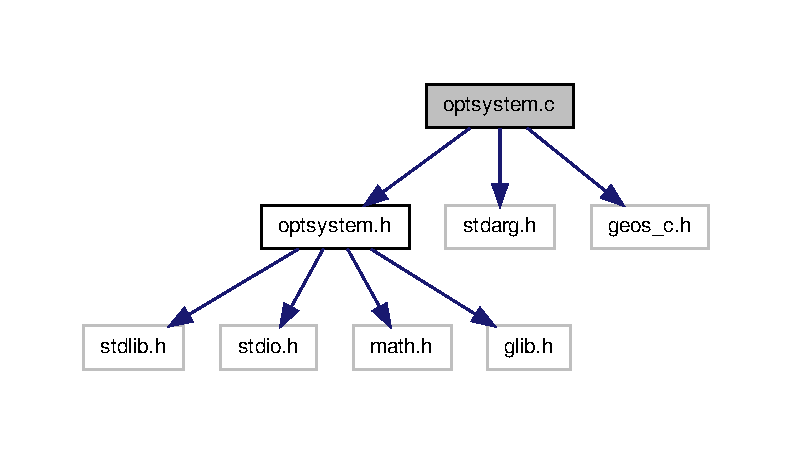
\includegraphics[width=350pt]{dc/d3c/a00028}
\end{center}
\end{figure}
\subsection*{\-Functions}
\begin{DoxyCompactItemize}
\item 
gboolean \hyperlink{a00017_a9f36fca086a6cf92613350b5b2d513a7_a9f36fca086a6cf92613350b5b2d513a7}{optsystem\-\_\-on\-\_\-obstacle} (\hyperlink{a00018_a48d08bbb4534f55ba817743a2b91360c_a48d08bbb4534f55ba817743a2b91360c}{optsystem\-\_\-t} $\ast$self, \hyperlink{a00018_a1c9d0bb39483d4981491e6383b0dbb47_a1c9d0bb39483d4981491e6383b0dbb47}{state\-\_\-t} $\ast$state)
\item 
int \hyperlink{a00017_ab593d0ccc2b4b49a7ba7a140505bdb5c_ab593d0ccc2b4b49a7ba7a140505bdb5c}{optsystem\-\_\-segment\-\_\-on\-\_\-obstacle} (\hyperlink{a00018_a48d08bbb4534f55ba817743a2b91360c_a48d08bbb4534f55ba817743a2b91360c}{optsystem\-\_\-t} $\ast$self, \hyperlink{a00018_a1c9d0bb39483d4981491e6383b0dbb47_a1c9d0bb39483d4981491e6383b0dbb47}{state\-\_\-t} $\ast$state\-\_\-initial, \hyperlink{a00018_a1c9d0bb39483d4981491e6383b0dbb47_a1c9d0bb39483d4981491e6383b0dbb47}{state\-\_\-t} $\ast$state\-\_\-final, int num\-\_\-steps)
\item 
int \hyperlink{a00017_ad37a0c28a54088a6415ad9dd85542379_ad37a0c28a54088a6415ad9dd85542379}{optsystem\-\_\-new\-\_\-system} (\hyperlink{a00018_a48d08bbb4534f55ba817743a2b91360c_a48d08bbb4534f55ba817743a2b91360c}{optsystem\-\_\-t} $\ast$self)
\item 
void \hyperlink{a00017_aa9b138e04bbc249582d169d3e3b710df_aa9b138e04bbc249582d169d3e3b710df}{notice} (const char $\ast$fmt,...)
\item 
void \hyperlink{a00017_afc84c983cb791517c5f8cdf61cd6bea0_afc84c983cb791517c5f8cdf61cd6bea0}{log\-\_\-and\-\_\-exit} (const char $\ast$fmt,...)
\item 
int \hyperlink{a00017_a1b54dac5618bcfadd941a7585239e52e_a1b54dac5618bcfadd941a7585239e52e}{optsystem\-\_\-free\-\_\-system} (\hyperlink{a00018_a48d08bbb4534f55ba817743a2b91360c_a48d08bbb4534f55ba817743a2b91360c}{optsystem\-\_\-t} $\ast$self)
\item 
\hyperlink{a00018_a1c9d0bb39483d4981491e6383b0dbb47_a1c9d0bb39483d4981491e6383b0dbb47}{state\-\_\-t} $\ast$ \hyperlink{a00017_a7eb5bfb9a16cf6e49245635fa2400465_a7eb5bfb9a16cf6e49245635fa2400465}{optsystem\-\_\-new\-\_\-state} (\hyperlink{a00018_a48d08bbb4534f55ba817743a2b91360c_a48d08bbb4534f55ba817743a2b91360c}{optsystem\-\_\-t} $\ast$self)
\item 
int \hyperlink{a00017_a27f43c59aba7a8c383399066481b18ba_a27f43c59aba7a8c383399066481b18ba}{optsystem\-\_\-free\-\_\-state} (\hyperlink{a00018_a48d08bbb4534f55ba817743a2b91360c_a48d08bbb4534f55ba817743a2b91360c}{optsystem\-\_\-t} $\ast$self, \hyperlink{a00018_a1c9d0bb39483d4981491e6383b0dbb47_a1c9d0bb39483d4981491e6383b0dbb47}{state\-\_\-t} $\ast$state)
\item 
\hyperlink{a00018_a8e5c489dcfacb9bd5f2985013638ea12_a8e5c489dcfacb9bd5f2985013638ea12}{input\-\_\-t} $\ast$ \hyperlink{a00017_ac249533c36b3db8e1236a3ede20c0be2_ac249533c36b3db8e1236a3ede20c0be2}{optsystem\-\_\-new\-\_\-input} (\hyperlink{a00018_a48d08bbb4534f55ba817743a2b91360c_a48d08bbb4534f55ba817743a2b91360c}{optsystem\-\_\-t} $\ast$self)
\item 
int \hyperlink{a00017_aa20115db43f7ad2bc631d4dee3faf439_aa20115db43f7ad2bc631d4dee3faf439}{optsystem\-\_\-free\-\_\-input} (\hyperlink{a00018_a48d08bbb4534f55ba817743a2b91360c_a48d08bbb4534f55ba817743a2b91360c}{optsystem\-\_\-t} $\ast$self, \hyperlink{a00018_a8e5c489dcfacb9bd5f2985013638ea12_a8e5c489dcfacb9bd5f2985013638ea12}{input\-\_\-t} $\ast$input)
\item 
\hyperlink{a00018_a1c9d0bb39483d4981491e6383b0dbb47_a1c9d0bb39483d4981491e6383b0dbb47}{state\-\_\-t} $\ast$ \hyperlink{a00017_adccdea6115438d8427e2969bffd8d87e_adccdea6115438d8427e2969bffd8d87e}{optsystem\-\_\-clone\-\_\-state} (\hyperlink{a00018_a48d08bbb4534f55ba817743a2b91360c_a48d08bbb4534f55ba817743a2b91360c}{optsystem\-\_\-t} $\ast$self, \hyperlink{a00018_a1c9d0bb39483d4981491e6383b0dbb47_a1c9d0bb39483d4981491e6383b0dbb47}{state\-\_\-t} $\ast$state)
\item 
int \hyperlink{a00017_a4b9f82df886ac6634d2ee9532b603163_a4b9f82df886ac6634d2ee9532b603163}{optsystem\-\_\-set\-\_\-initial\-\_\-state} (\hyperlink{a00018_a48d08bbb4534f55ba817743a2b91360c_a48d08bbb4534f55ba817743a2b91360c}{optsystem\-\_\-t} $\ast$self, \hyperlink{a00018_a1c9d0bb39483d4981491e6383b0dbb47_a1c9d0bb39483d4981491e6383b0dbb47}{state\-\_\-t} $\ast$state)
\item 
int \hyperlink{a00017_ad414a4b37c77f9e4324071ee6fc1c1b8_ad414a4b37c77f9e4324071ee6fc1c1b8}{optsystem\-\_\-get\-\_\-initial\-\_\-state} (\hyperlink{a00018_a48d08bbb4534f55ba817743a2b91360c_a48d08bbb4534f55ba817743a2b91360c}{optsystem\-\_\-t} $\ast$self, \hyperlink{a00018_a1c9d0bb39483d4981491e6383b0dbb47_a1c9d0bb39483d4981491e6383b0dbb47}{state\-\_\-t} $\ast$state)
\item 
int \hyperlink{a00017_aa8d351156d5b945f766be43089c406e4_aa8d351156d5b945f766be43089c406e4}{optsystem\-\_\-get\-\_\-num\-\_\-states} (\hyperlink{a00018_a48d08bbb4534f55ba817743a2b91360c_a48d08bbb4534f55ba817743a2b91360c}{optsystem\-\_\-t} $\ast$self)
\item 
double $\ast$ \hyperlink{a00017_a4748b851e592ba16255987990df866dc_a4748b851e592ba16255987990df866dc}{optsystem\-\_\-get\-\_\-state\-\_\-key} (\hyperlink{a00018_a48d08bbb4534f55ba817743a2b91360c_a48d08bbb4534f55ba817743a2b91360c}{optsystem\-\_\-t} $\ast$self, \hyperlink{a00018_a1c9d0bb39483d4981491e6383b0dbb47_a1c9d0bb39483d4981491e6383b0dbb47}{state\-\_\-t} $\ast$state)
\item 
int \hyperlink{a00017_a778500228810cbc69a6d17494f889b87_a778500228810cbc69a6d17494f889b87}{optsystem\-\_\-sample\-\_\-state} (\hyperlink{a00018_a48d08bbb4534f55ba817743a2b91360c_a48d08bbb4534f55ba817743a2b91360c}{optsystem\-\_\-t} $\ast$self, \hyperlink{a00018_a1c9d0bb39483d4981491e6383b0dbb47_a1c9d0bb39483d4981491e6383b0dbb47}{state\-\_\-t} $\ast$random\-\_\-state)
\item 
int \hyperlink{a00017_a2294e6525f29f89ef7c0e3424063df15_a2294e6525f29f89ef7c0e3424063df15}{optsystem\-\_\-sample\-\_\-target\-\_\-state} (\hyperlink{a00018_a48d08bbb4534f55ba817743a2b91360c_a48d08bbb4534f55ba817743a2b91360c}{optsystem\-\_\-t} $\ast$self, \hyperlink{a00018_a1c9d0bb39483d4981491e6383b0dbb47_a1c9d0bb39483d4981491e6383b0dbb47}{state\-\_\-t} $\ast$random\-\_\-state)
\item 
double \hyperlink{a00017_afce48612176b92f14cb7ffcc91259454_afce48612176b92f14cb7ffcc91259454}{optsystem\-\_\-evaluate\-\_\-distance} (\hyperlink{a00018_a48d08bbb4534f55ba817743a2b91360c_a48d08bbb4534f55ba817743a2b91360c}{optsystem\-\_\-t} $\ast$self, \hyperlink{a00018_a1c9d0bb39483d4981491e6383b0dbb47_a1c9d0bb39483d4981491e6383b0dbb47}{state\-\_\-t} $\ast$state\-\_\-from, \hyperlink{a00018_a1c9d0bb39483d4981491e6383b0dbb47_a1c9d0bb39483d4981491e6383b0dbb47}{state\-\_\-t} $\ast$state\-\_\-to)
\item 
double \hyperlink{a00017_acb788463670e5a6ef08d3759e8fc22ba_acb788463670e5a6ef08d3759e8fc22ba}{optsystem\-\_\-evaluate\-\_\-distance\-\_\-for\-\_\-cost} (\hyperlink{a00018_a48d08bbb4534f55ba817743a2b91360c_a48d08bbb4534f55ba817743a2b91360c}{optsystem\-\_\-t} $\ast$self, \-G\-S\-List $\ast$inputs)
\item 
int \hyperlink{a00017_a10f9c56911d68043e9357824ef0440bc_a10f9c56911d68043e9357824ef0440bc}{optsystem\-\_\-extend\-\_\-to} (\hyperlink{a00018_a48d08bbb4534f55ba817743a2b91360c_a48d08bbb4534f55ba817743a2b91360c}{optsystem\-\_\-t} $\ast$self, \hyperlink{a00018_a1c9d0bb39483d4981491e6383b0dbb47_a1c9d0bb39483d4981491e6383b0dbb47}{state\-\_\-t} $\ast$state\-\_\-from, \hyperlink{a00018_a1c9d0bb39483d4981491e6383b0dbb47_a1c9d0bb39483d4981491e6383b0dbb47}{state\-\_\-t} $\ast$state\-\_\-towards, int $\ast$fully\-\_\-extends, \-G\-S\-List $\ast$$\ast$trajectory, int $\ast$num\-\_\-node\-\_\-states, int $\ast$$\ast$nodes\-\_\-states, \-G\-S\-List $\ast$$\ast$inputs)
\item 
gboolean \hyperlink{a00017_a6e1675238ed175e198390a142a966fbb_a6e1675238ed175e198390a142a966fbb}{optsystem\-\_\-is\-\_\-reaching\-\_\-target} (\hyperlink{a00018_a48d08bbb4534f55ba817743a2b91360c_a48d08bbb4534f55ba817743a2b91360c}{optsystem\-\_\-t} $\ast$self, \hyperlink{a00018_a1c9d0bb39483d4981491e6383b0dbb47_a1c9d0bb39483d4981491e6383b0dbb47}{state\-\_\-t} $\ast$state)
\item 
double \hyperlink{a00017_a1ae2c2cb3d755ea6b5465a6e3a015af0_a1ae2c2cb3d755ea6b5465a6e3a015af0}{optsystem\-\_\-evaluate\-\_\-cost\-\_\-to\-\_\-go} (\hyperlink{a00018_a48d08bbb4534f55ba817743a2b91360c_a48d08bbb4534f55ba817743a2b91360c}{optsystem\-\_\-t} $\ast$self, \hyperlink{a00018_a1c9d0bb39483d4981491e6383b0dbb47_a1c9d0bb39483d4981491e6383b0dbb47}{state\-\_\-t} $\ast$state)
\item 
gboolean \hyperlink{a00017_a086fb96570b474b5658dc991c8becc79_a086fb96570b474b5658dc991c8becc79}{optsystem\-\_\-update\-\_\-goal\-\_\-region} (\hyperlink{a00018_a48d08bbb4534f55ba817743a2b91360c_a48d08bbb4534f55ba817743a2b91360c}{optsystem\-\_\-t} $\ast$self, \hyperlink{a00018_a9136102e25aac8406a94d89f5a95bd1f_a9136102e25aac8406a94d89f5a95bd1f}{region\-\_\-2d\-\_\-t} $\ast$goal\-\_\-region)
\item 
gboolean \hyperlink{a00017_a3af82be1a1df5324149ee8a6450e0381_a3af82be1a1df5324149ee8a6450e0381}{optsystem\-\_\-update\-\_\-operating\-\_\-region} (\hyperlink{a00018_a48d08bbb4534f55ba817743a2b91360c_a48d08bbb4534f55ba817743a2b91360c}{optsystem\-\_\-t} $\ast$self, \hyperlink{a00018_a9136102e25aac8406a94d89f5a95bd1f_a9136102e25aac8406a94d89f5a95bd1f}{region\-\_\-2d\-\_\-t} $\ast$operating\-\_\-region)
\item 
gboolean \hyperlink{a00017_a0ad4a450490357b767cd191a83d2cdec_a0ad4a450490357b767cd191a83d2cdec}{optsystem\-\_\-update\-\_\-obstacles} (\hyperlink{a00018_a48d08bbb4534f55ba817743a2b91360c_a48d08bbb4534f55ba817743a2b91360c}{optsystem\-\_\-t} $\ast$self, \-G\-S\-List $\ast$obstacle\-\_\-list)
\item 
gboolean \hyperlink{a00017_afaee017543d17527597efd3a34a7c317_afaee017543d17527597efd3a34a7c317}{optsystem\-\_\-update\-\_\-rectangles} (\hyperlink{a00018_a48d08bbb4534f55ba817743a2b91360c_a48d08bbb4534f55ba817743a2b91360c}{optsystem\-\_\-t} $\ast$self, \-G\-S\-List $\ast$rectangle\-\_\-list)
\end{DoxyCompactItemize}


\subsection{\-Function \-Documentation}
\hypertarget{a00017_afc84c983cb791517c5f8cdf61cd6bea0_afc84c983cb791517c5f8cdf61cd6bea0}{\index{optsystem.\-c@{optsystem.\-c}!log\-\_\-and\-\_\-exit@{log\-\_\-and\-\_\-exit}}
\index{log\-\_\-and\-\_\-exit@{log\-\_\-and\-\_\-exit}!optsystem.c@{optsystem.\-c}}
\subsubsection[{log\-\_\-and\-\_\-exit}]{\setlength{\rightskip}{0pt plus 5cm}void {\bf log\-\_\-and\-\_\-exit} (
\begin{DoxyParamCaption}
\item[{const char $\ast$}]{fmt, }
\item[{}]{...}
\end{DoxyParamCaption}
)}}\label{d4/d51/a00017_afc84c983cb791517c5f8cdf61cd6bea0_afc84c983cb791517c5f8cdf61cd6bea0}
\hypertarget{a00017_aa9b138e04bbc249582d169d3e3b710df_aa9b138e04bbc249582d169d3e3b710df}{\index{optsystem.\-c@{optsystem.\-c}!notice@{notice}}
\index{notice@{notice}!optsystem.c@{optsystem.\-c}}
\subsubsection[{notice}]{\setlength{\rightskip}{0pt plus 5cm}void {\bf notice} (
\begin{DoxyParamCaption}
\item[{const char $\ast$}]{fmt, }
\item[{}]{...}
\end{DoxyParamCaption}
)}}\label{d4/d51/a00017_aa9b138e04bbc249582d169d3e3b710df_aa9b138e04bbc249582d169d3e3b710df}
\hypertarget{a00017_adccdea6115438d8427e2969bffd8d87e_adccdea6115438d8427e2969bffd8d87e}{\index{optsystem.\-c@{optsystem.\-c}!optsystem\-\_\-clone\-\_\-state@{optsystem\-\_\-clone\-\_\-state}}
\index{optsystem\-\_\-clone\-\_\-state@{optsystem\-\_\-clone\-\_\-state}!optsystem.c@{optsystem.\-c}}
\subsubsection[{optsystem\-\_\-clone\-\_\-state}]{\setlength{\rightskip}{0pt plus 5cm}{\bf state\-\_\-t}$\ast$ {\bf optsystem\-\_\-clone\-\_\-state} (
\begin{DoxyParamCaption}
\item[{{\bf optsystem\-\_\-t} $\ast$}]{self, }
\item[{{\bf state\-\_\-t} $\ast$}]{state}
\end{DoxyParamCaption}
)}}\label{d4/d51/a00017_adccdea6115438d8427e2969bffd8d87e_adccdea6115438d8427e2969bffd8d87e}
\hypertarget{a00017_a1ae2c2cb3d755ea6b5465a6e3a015af0_a1ae2c2cb3d755ea6b5465a6e3a015af0}{\index{optsystem.\-c@{optsystem.\-c}!optsystem\-\_\-evaluate\-\_\-cost\-\_\-to\-\_\-go@{optsystem\-\_\-evaluate\-\_\-cost\-\_\-to\-\_\-go}}
\index{optsystem\-\_\-evaluate\-\_\-cost\-\_\-to\-\_\-go@{optsystem\-\_\-evaluate\-\_\-cost\-\_\-to\-\_\-go}!optsystem.c@{optsystem.\-c}}
\subsubsection[{optsystem\-\_\-evaluate\-\_\-cost\-\_\-to\-\_\-go}]{\setlength{\rightskip}{0pt plus 5cm}double {\bf optsystem\-\_\-evaluate\-\_\-cost\-\_\-to\-\_\-go} (
\begin{DoxyParamCaption}
\item[{{\bf optsystem\-\_\-t} $\ast$}]{self, }
\item[{{\bf state\-\_\-t} $\ast$}]{state}
\end{DoxyParamCaption}
)}}\label{d4/d51/a00017_a1ae2c2cb3d755ea6b5465a6e3a015af0_a1ae2c2cb3d755ea6b5465a6e3a015af0}
\hypertarget{a00017_afce48612176b92f14cb7ffcc91259454_afce48612176b92f14cb7ffcc91259454}{\index{optsystem.\-c@{optsystem.\-c}!optsystem\-\_\-evaluate\-\_\-distance@{optsystem\-\_\-evaluate\-\_\-distance}}
\index{optsystem\-\_\-evaluate\-\_\-distance@{optsystem\-\_\-evaluate\-\_\-distance}!optsystem.c@{optsystem.\-c}}
\subsubsection[{optsystem\-\_\-evaluate\-\_\-distance}]{\setlength{\rightskip}{0pt plus 5cm}double {\bf optsystem\-\_\-evaluate\-\_\-distance} (
\begin{DoxyParamCaption}
\item[{{\bf optsystem\-\_\-t} $\ast$}]{self, }
\item[{{\bf state\-\_\-t} $\ast$}]{state\-\_\-from, }
\item[{{\bf state\-\_\-t} $\ast$}]{state\-\_\-to}
\end{DoxyParamCaption}
)}}\label{d4/d51/a00017_afce48612176b92f14cb7ffcc91259454_afce48612176b92f14cb7ffcc91259454}
\hypertarget{a00017_acb788463670e5a6ef08d3759e8fc22ba_acb788463670e5a6ef08d3759e8fc22ba}{\index{optsystem.\-c@{optsystem.\-c}!optsystem\-\_\-evaluate\-\_\-distance\-\_\-for\-\_\-cost@{optsystem\-\_\-evaluate\-\_\-distance\-\_\-for\-\_\-cost}}
\index{optsystem\-\_\-evaluate\-\_\-distance\-\_\-for\-\_\-cost@{optsystem\-\_\-evaluate\-\_\-distance\-\_\-for\-\_\-cost}!optsystem.c@{optsystem.\-c}}
\subsubsection[{optsystem\-\_\-evaluate\-\_\-distance\-\_\-for\-\_\-cost}]{\setlength{\rightskip}{0pt plus 5cm}double {\bf optsystem\-\_\-evaluate\-\_\-distance\-\_\-for\-\_\-cost} (
\begin{DoxyParamCaption}
\item[{{\bf optsystem\-\_\-t} $\ast$}]{self, }
\item[{\-G\-S\-List $\ast$}]{inputs}
\end{DoxyParamCaption}
)}}\label{d4/d51/a00017_acb788463670e5a6ef08d3759e8fc22ba_acb788463670e5a6ef08d3759e8fc22ba}
\hypertarget{a00017_a10f9c56911d68043e9357824ef0440bc_a10f9c56911d68043e9357824ef0440bc}{\index{optsystem.\-c@{optsystem.\-c}!optsystem\-\_\-extend\-\_\-to@{optsystem\-\_\-extend\-\_\-to}}
\index{optsystem\-\_\-extend\-\_\-to@{optsystem\-\_\-extend\-\_\-to}!optsystem.c@{optsystem.\-c}}
\subsubsection[{optsystem\-\_\-extend\-\_\-to}]{\setlength{\rightskip}{0pt plus 5cm}int {\bf optsystem\-\_\-extend\-\_\-to} (
\begin{DoxyParamCaption}
\item[{{\bf optsystem\-\_\-t} $\ast$}]{self, }
\item[{{\bf state\-\_\-t} $\ast$}]{state\-\_\-from, }
\item[{{\bf state\-\_\-t} $\ast$}]{state\-\_\-towards, }
\item[{int $\ast$}]{fully\-\_\-extends, }
\item[{\-G\-S\-List $\ast$$\ast$}]{trajectory, }
\item[{int $\ast$}]{num\-\_\-node\-\_\-states, }
\item[{int $\ast$$\ast$}]{nodes\-\_\-states, }
\item[{\-G\-S\-List $\ast$$\ast$}]{inputs}
\end{DoxyParamCaption}
)}}\label{d4/d51/a00017_a10f9c56911d68043e9357824ef0440bc_a10f9c56911d68043e9357824ef0440bc}
\hypertarget{a00017_aa20115db43f7ad2bc631d4dee3faf439_aa20115db43f7ad2bc631d4dee3faf439}{\index{optsystem.\-c@{optsystem.\-c}!optsystem\-\_\-free\-\_\-input@{optsystem\-\_\-free\-\_\-input}}
\index{optsystem\-\_\-free\-\_\-input@{optsystem\-\_\-free\-\_\-input}!optsystem.c@{optsystem.\-c}}
\subsubsection[{optsystem\-\_\-free\-\_\-input}]{\setlength{\rightskip}{0pt plus 5cm}int {\bf optsystem\-\_\-free\-\_\-input} (
\begin{DoxyParamCaption}
\item[{{\bf optsystem\-\_\-t} $\ast$}]{self, }
\item[{{\bf input\-\_\-t} $\ast$}]{input}
\end{DoxyParamCaption}
)}}\label{d4/d51/a00017_aa20115db43f7ad2bc631d4dee3faf439_aa20115db43f7ad2bc631d4dee3faf439}
\hypertarget{a00017_a27f43c59aba7a8c383399066481b18ba_a27f43c59aba7a8c383399066481b18ba}{\index{optsystem.\-c@{optsystem.\-c}!optsystem\-\_\-free\-\_\-state@{optsystem\-\_\-free\-\_\-state}}
\index{optsystem\-\_\-free\-\_\-state@{optsystem\-\_\-free\-\_\-state}!optsystem.c@{optsystem.\-c}}
\subsubsection[{optsystem\-\_\-free\-\_\-state}]{\setlength{\rightskip}{0pt plus 5cm}int {\bf optsystem\-\_\-free\-\_\-state} (
\begin{DoxyParamCaption}
\item[{{\bf optsystem\-\_\-t} $\ast$}]{self, }
\item[{{\bf state\-\_\-t} $\ast$}]{state}
\end{DoxyParamCaption}
)}}\label{d4/d51/a00017_a27f43c59aba7a8c383399066481b18ba_a27f43c59aba7a8c383399066481b18ba}
\hypertarget{a00017_a1b54dac5618bcfadd941a7585239e52e_a1b54dac5618bcfadd941a7585239e52e}{\index{optsystem.\-c@{optsystem.\-c}!optsystem\-\_\-free\-\_\-system@{optsystem\-\_\-free\-\_\-system}}
\index{optsystem\-\_\-free\-\_\-system@{optsystem\-\_\-free\-\_\-system}!optsystem.c@{optsystem.\-c}}
\subsubsection[{optsystem\-\_\-free\-\_\-system}]{\setlength{\rightskip}{0pt plus 5cm}int {\bf optsystem\-\_\-free\-\_\-system} (
\begin{DoxyParamCaption}
\item[{{\bf optsystem\-\_\-t} $\ast$}]{self}
\end{DoxyParamCaption}
)}}\label{d4/d51/a00017_a1b54dac5618bcfadd941a7585239e52e_a1b54dac5618bcfadd941a7585239e52e}
\hypertarget{a00017_ad414a4b37c77f9e4324071ee6fc1c1b8_ad414a4b37c77f9e4324071ee6fc1c1b8}{\index{optsystem.\-c@{optsystem.\-c}!optsystem\-\_\-get\-\_\-initial\-\_\-state@{optsystem\-\_\-get\-\_\-initial\-\_\-state}}
\index{optsystem\-\_\-get\-\_\-initial\-\_\-state@{optsystem\-\_\-get\-\_\-initial\-\_\-state}!optsystem.c@{optsystem.\-c}}
\subsubsection[{optsystem\-\_\-get\-\_\-initial\-\_\-state}]{\setlength{\rightskip}{0pt plus 5cm}int {\bf optsystem\-\_\-get\-\_\-initial\-\_\-state} (
\begin{DoxyParamCaption}
\item[{{\bf optsystem\-\_\-t} $\ast$}]{self, }
\item[{{\bf state\-\_\-t} $\ast$}]{state}
\end{DoxyParamCaption}
)}}\label{d4/d51/a00017_ad414a4b37c77f9e4324071ee6fc1c1b8_ad414a4b37c77f9e4324071ee6fc1c1b8}
\hypertarget{a00017_aa8d351156d5b945f766be43089c406e4_aa8d351156d5b945f766be43089c406e4}{\index{optsystem.\-c@{optsystem.\-c}!optsystem\-\_\-get\-\_\-num\-\_\-states@{optsystem\-\_\-get\-\_\-num\-\_\-states}}
\index{optsystem\-\_\-get\-\_\-num\-\_\-states@{optsystem\-\_\-get\-\_\-num\-\_\-states}!optsystem.c@{optsystem.\-c}}
\subsubsection[{optsystem\-\_\-get\-\_\-num\-\_\-states}]{\setlength{\rightskip}{0pt plus 5cm}int {\bf optsystem\-\_\-get\-\_\-num\-\_\-states} (
\begin{DoxyParamCaption}
\item[{{\bf optsystem\-\_\-t} $\ast$}]{self}
\end{DoxyParamCaption}
)}}\label{d4/d51/a00017_aa8d351156d5b945f766be43089c406e4_aa8d351156d5b945f766be43089c406e4}
\hypertarget{a00017_a4748b851e592ba16255987990df866dc_a4748b851e592ba16255987990df866dc}{\index{optsystem.\-c@{optsystem.\-c}!optsystem\-\_\-get\-\_\-state\-\_\-key@{optsystem\-\_\-get\-\_\-state\-\_\-key}}
\index{optsystem\-\_\-get\-\_\-state\-\_\-key@{optsystem\-\_\-get\-\_\-state\-\_\-key}!optsystem.c@{optsystem.\-c}}
\subsubsection[{optsystem\-\_\-get\-\_\-state\-\_\-key}]{\setlength{\rightskip}{0pt plus 5cm}double$\ast$ {\bf optsystem\-\_\-get\-\_\-state\-\_\-key} (
\begin{DoxyParamCaption}
\item[{{\bf optsystem\-\_\-t} $\ast$}]{self, }
\item[{{\bf state\-\_\-t} $\ast$}]{state}
\end{DoxyParamCaption}
)}}\label{d4/d51/a00017_a4748b851e592ba16255987990df866dc_a4748b851e592ba16255987990df866dc}
\hypertarget{a00017_a6e1675238ed175e198390a142a966fbb_a6e1675238ed175e198390a142a966fbb}{\index{optsystem.\-c@{optsystem.\-c}!optsystem\-\_\-is\-\_\-reaching\-\_\-target@{optsystem\-\_\-is\-\_\-reaching\-\_\-target}}
\index{optsystem\-\_\-is\-\_\-reaching\-\_\-target@{optsystem\-\_\-is\-\_\-reaching\-\_\-target}!optsystem.c@{optsystem.\-c}}
\subsubsection[{optsystem\-\_\-is\-\_\-reaching\-\_\-target}]{\setlength{\rightskip}{0pt plus 5cm}gboolean {\bf optsystem\-\_\-is\-\_\-reaching\-\_\-target} (
\begin{DoxyParamCaption}
\item[{{\bf optsystem\-\_\-t} $\ast$}]{self, }
\item[{{\bf state\-\_\-t} $\ast$}]{state}
\end{DoxyParamCaption}
)}}\label{d4/d51/a00017_a6e1675238ed175e198390a142a966fbb_a6e1675238ed175e198390a142a966fbb}
\hypertarget{a00017_ac249533c36b3db8e1236a3ede20c0be2_ac249533c36b3db8e1236a3ede20c0be2}{\index{optsystem.\-c@{optsystem.\-c}!optsystem\-\_\-new\-\_\-input@{optsystem\-\_\-new\-\_\-input}}
\index{optsystem\-\_\-new\-\_\-input@{optsystem\-\_\-new\-\_\-input}!optsystem.c@{optsystem.\-c}}
\subsubsection[{optsystem\-\_\-new\-\_\-input}]{\setlength{\rightskip}{0pt plus 5cm}{\bf input\-\_\-t}$\ast$ {\bf optsystem\-\_\-new\-\_\-input} (
\begin{DoxyParamCaption}
\item[{{\bf optsystem\-\_\-t} $\ast$}]{self}
\end{DoxyParamCaption}
)}}\label{d4/d51/a00017_ac249533c36b3db8e1236a3ede20c0be2_ac249533c36b3db8e1236a3ede20c0be2}
\hypertarget{a00017_a7eb5bfb9a16cf6e49245635fa2400465_a7eb5bfb9a16cf6e49245635fa2400465}{\index{optsystem.\-c@{optsystem.\-c}!optsystem\-\_\-new\-\_\-state@{optsystem\-\_\-new\-\_\-state}}
\index{optsystem\-\_\-new\-\_\-state@{optsystem\-\_\-new\-\_\-state}!optsystem.c@{optsystem.\-c}}
\subsubsection[{optsystem\-\_\-new\-\_\-state}]{\setlength{\rightskip}{0pt plus 5cm}{\bf state\-\_\-t}$\ast$ {\bf optsystem\-\_\-new\-\_\-state} (
\begin{DoxyParamCaption}
\item[{{\bf optsystem\-\_\-t} $\ast$}]{self}
\end{DoxyParamCaption}
)}}\label{d4/d51/a00017_a7eb5bfb9a16cf6e49245635fa2400465_a7eb5bfb9a16cf6e49245635fa2400465}
\hypertarget{a00017_ad37a0c28a54088a6415ad9dd85542379_ad37a0c28a54088a6415ad9dd85542379}{\index{optsystem.\-c@{optsystem.\-c}!optsystem\-\_\-new\-\_\-system@{optsystem\-\_\-new\-\_\-system}}
\index{optsystem\-\_\-new\-\_\-system@{optsystem\-\_\-new\-\_\-system}!optsystem.c@{optsystem.\-c}}
\subsubsection[{optsystem\-\_\-new\-\_\-system}]{\setlength{\rightskip}{0pt plus 5cm}int {\bf optsystem\-\_\-new\-\_\-system} (
\begin{DoxyParamCaption}
\item[{{\bf optsystem\-\_\-t} $\ast$}]{self}
\end{DoxyParamCaption}
)}}\label{d4/d51/a00017_ad37a0c28a54088a6415ad9dd85542379_ad37a0c28a54088a6415ad9dd85542379}
\hypertarget{a00017_a9f36fca086a6cf92613350b5b2d513a7_a9f36fca086a6cf92613350b5b2d513a7}{\index{optsystem.\-c@{optsystem.\-c}!optsystem\-\_\-on\-\_\-obstacle@{optsystem\-\_\-on\-\_\-obstacle}}
\index{optsystem\-\_\-on\-\_\-obstacle@{optsystem\-\_\-on\-\_\-obstacle}!optsystem.c@{optsystem.\-c}}
\subsubsection[{optsystem\-\_\-on\-\_\-obstacle}]{\setlength{\rightskip}{0pt plus 5cm}gboolean {\bf optsystem\-\_\-on\-\_\-obstacle} (
\begin{DoxyParamCaption}
\item[{{\bf optsystem\-\_\-t} $\ast$}]{self, }
\item[{{\bf state\-\_\-t} $\ast$}]{state}
\end{DoxyParamCaption}
)}}\label{d4/d51/a00017_a9f36fca086a6cf92613350b5b2d513a7_a9f36fca086a6cf92613350b5b2d513a7}
\hypertarget{a00017_a778500228810cbc69a6d17494f889b87_a778500228810cbc69a6d17494f889b87}{\index{optsystem.\-c@{optsystem.\-c}!optsystem\-\_\-sample\-\_\-state@{optsystem\-\_\-sample\-\_\-state}}
\index{optsystem\-\_\-sample\-\_\-state@{optsystem\-\_\-sample\-\_\-state}!optsystem.c@{optsystem.\-c}}
\subsubsection[{optsystem\-\_\-sample\-\_\-state}]{\setlength{\rightskip}{0pt plus 5cm}int {\bf optsystem\-\_\-sample\-\_\-state} (
\begin{DoxyParamCaption}
\item[{{\bf optsystem\-\_\-t} $\ast$}]{self, }
\item[{{\bf state\-\_\-t} $\ast$}]{random\-\_\-state}
\end{DoxyParamCaption}
)}}\label{d4/d51/a00017_a778500228810cbc69a6d17494f889b87_a778500228810cbc69a6d17494f889b87}
\hypertarget{a00017_a2294e6525f29f89ef7c0e3424063df15_a2294e6525f29f89ef7c0e3424063df15}{\index{optsystem.\-c@{optsystem.\-c}!optsystem\-\_\-sample\-\_\-target\-\_\-state@{optsystem\-\_\-sample\-\_\-target\-\_\-state}}
\index{optsystem\-\_\-sample\-\_\-target\-\_\-state@{optsystem\-\_\-sample\-\_\-target\-\_\-state}!optsystem.c@{optsystem.\-c}}
\subsubsection[{optsystem\-\_\-sample\-\_\-target\-\_\-state}]{\setlength{\rightskip}{0pt plus 5cm}int {\bf optsystem\-\_\-sample\-\_\-target\-\_\-state} (
\begin{DoxyParamCaption}
\item[{{\bf optsystem\-\_\-t} $\ast$}]{self, }
\item[{{\bf state\-\_\-t} $\ast$}]{random\-\_\-state}
\end{DoxyParamCaption}
)}}\label{d4/d51/a00017_a2294e6525f29f89ef7c0e3424063df15_a2294e6525f29f89ef7c0e3424063df15}
\hypertarget{a00017_ab593d0ccc2b4b49a7ba7a140505bdb5c_ab593d0ccc2b4b49a7ba7a140505bdb5c}{\index{optsystem.\-c@{optsystem.\-c}!optsystem\-\_\-segment\-\_\-on\-\_\-obstacle@{optsystem\-\_\-segment\-\_\-on\-\_\-obstacle}}
\index{optsystem\-\_\-segment\-\_\-on\-\_\-obstacle@{optsystem\-\_\-segment\-\_\-on\-\_\-obstacle}!optsystem.c@{optsystem.\-c}}
\subsubsection[{optsystem\-\_\-segment\-\_\-on\-\_\-obstacle}]{\setlength{\rightskip}{0pt plus 5cm}int {\bf optsystem\-\_\-segment\-\_\-on\-\_\-obstacle} (
\begin{DoxyParamCaption}
\item[{{\bf optsystem\-\_\-t} $\ast$}]{self, }
\item[{{\bf state\-\_\-t} $\ast$}]{state\-\_\-initial, }
\item[{{\bf state\-\_\-t} $\ast$}]{state\-\_\-final, }
\item[{int}]{num\-\_\-steps}
\end{DoxyParamCaption}
)}}\label{d4/d51/a00017_ab593d0ccc2b4b49a7ba7a140505bdb5c_ab593d0ccc2b4b49a7ba7a140505bdb5c}
\hypertarget{a00017_a4b9f82df886ac6634d2ee9532b603163_a4b9f82df886ac6634d2ee9532b603163}{\index{optsystem.\-c@{optsystem.\-c}!optsystem\-\_\-set\-\_\-initial\-\_\-state@{optsystem\-\_\-set\-\_\-initial\-\_\-state}}
\index{optsystem\-\_\-set\-\_\-initial\-\_\-state@{optsystem\-\_\-set\-\_\-initial\-\_\-state}!optsystem.c@{optsystem.\-c}}
\subsubsection[{optsystem\-\_\-set\-\_\-initial\-\_\-state}]{\setlength{\rightskip}{0pt plus 5cm}int {\bf optsystem\-\_\-set\-\_\-initial\-\_\-state} (
\begin{DoxyParamCaption}
\item[{{\bf optsystem\-\_\-t} $\ast$}]{self, }
\item[{{\bf state\-\_\-t} $\ast$}]{state}
\end{DoxyParamCaption}
)}}\label{d4/d51/a00017_a4b9f82df886ac6634d2ee9532b603163_a4b9f82df886ac6634d2ee9532b603163}
\hypertarget{a00017_a086fb96570b474b5658dc991c8becc79_a086fb96570b474b5658dc991c8becc79}{\index{optsystem.\-c@{optsystem.\-c}!optsystem\-\_\-update\-\_\-goal\-\_\-region@{optsystem\-\_\-update\-\_\-goal\-\_\-region}}
\index{optsystem\-\_\-update\-\_\-goal\-\_\-region@{optsystem\-\_\-update\-\_\-goal\-\_\-region}!optsystem.c@{optsystem.\-c}}
\subsubsection[{optsystem\-\_\-update\-\_\-goal\-\_\-region}]{\setlength{\rightskip}{0pt plus 5cm}gboolean {\bf optsystem\-\_\-update\-\_\-goal\-\_\-region} (
\begin{DoxyParamCaption}
\item[{{\bf optsystem\-\_\-t} $\ast$}]{self, }
\item[{{\bf region\-\_\-2d\-\_\-t} $\ast$}]{goal\-\_\-region}
\end{DoxyParamCaption}
)}}\label{d4/d51/a00017_a086fb96570b474b5658dc991c8becc79_a086fb96570b474b5658dc991c8becc79}
\hypertarget{a00017_a0ad4a450490357b767cd191a83d2cdec_a0ad4a450490357b767cd191a83d2cdec}{\index{optsystem.\-c@{optsystem.\-c}!optsystem\-\_\-update\-\_\-obstacles@{optsystem\-\_\-update\-\_\-obstacles}}
\index{optsystem\-\_\-update\-\_\-obstacles@{optsystem\-\_\-update\-\_\-obstacles}!optsystem.c@{optsystem.\-c}}
\subsubsection[{optsystem\-\_\-update\-\_\-obstacles}]{\setlength{\rightskip}{0pt plus 5cm}gboolean {\bf optsystem\-\_\-update\-\_\-obstacles} (
\begin{DoxyParamCaption}
\item[{{\bf optsystem\-\_\-t} $\ast$}]{self, }
\item[{\-G\-S\-List $\ast$}]{obstacle\-\_\-list}
\end{DoxyParamCaption}
)}}\label{d4/d51/a00017_a0ad4a450490357b767cd191a83d2cdec_a0ad4a450490357b767cd191a83d2cdec}
\hypertarget{a00017_a3af82be1a1df5324149ee8a6450e0381_a3af82be1a1df5324149ee8a6450e0381}{\index{optsystem.\-c@{optsystem.\-c}!optsystem\-\_\-update\-\_\-operating\-\_\-region@{optsystem\-\_\-update\-\_\-operating\-\_\-region}}
\index{optsystem\-\_\-update\-\_\-operating\-\_\-region@{optsystem\-\_\-update\-\_\-operating\-\_\-region}!optsystem.c@{optsystem.\-c}}
\subsubsection[{optsystem\-\_\-update\-\_\-operating\-\_\-region}]{\setlength{\rightskip}{0pt plus 5cm}gboolean {\bf optsystem\-\_\-update\-\_\-operating\-\_\-region} (
\begin{DoxyParamCaption}
\item[{{\bf optsystem\-\_\-t} $\ast$}]{self, }
\item[{{\bf region\-\_\-2d\-\_\-t} $\ast$}]{operating\-\_\-region}
\end{DoxyParamCaption}
)}}\label{d4/d51/a00017_a3af82be1a1df5324149ee8a6450e0381_a3af82be1a1df5324149ee8a6450e0381}
\hypertarget{a00017_afaee017543d17527597efd3a34a7c317_afaee017543d17527597efd3a34a7c317}{\index{optsystem.\-c@{optsystem.\-c}!optsystem\-\_\-update\-\_\-rectangles@{optsystem\-\_\-update\-\_\-rectangles}}
\index{optsystem\-\_\-update\-\_\-rectangles@{optsystem\-\_\-update\-\_\-rectangles}!optsystem.c@{optsystem.\-c}}
\subsubsection[{optsystem\-\_\-update\-\_\-rectangles}]{\setlength{\rightskip}{0pt plus 5cm}gboolean {\bf optsystem\-\_\-update\-\_\-rectangles} (
\begin{DoxyParamCaption}
\item[{{\bf optsystem\-\_\-t} $\ast$}]{self, }
\item[{\-G\-S\-List $\ast$}]{rectangle\-\_\-list}
\end{DoxyParamCaption}
)}}\label{d4/d51/a00017_afaee017543d17527597efd3a34a7c317_afaee017543d17527597efd3a34a7c317}

\hypertarget{a00018}{\section{optsystem.\-h \-File \-Reference}
\label{d1/d2b/a00018}\index{optsystem.\-h@{optsystem.\-h}}
}
{\ttfamily \#include $<$stdlib.\-h$>$}\*
{\ttfamily \#include $<$stdio.\-h$>$}\*
{\ttfamily \#include $<$math.\-h$>$}\*
{\ttfamily \#include $<$glib.\-h$>$}\*
\-Include dependency graph for optsystem.\-h\-:\nopagebreak
\begin{figure}[H]
\begin{center}
\leavevmode
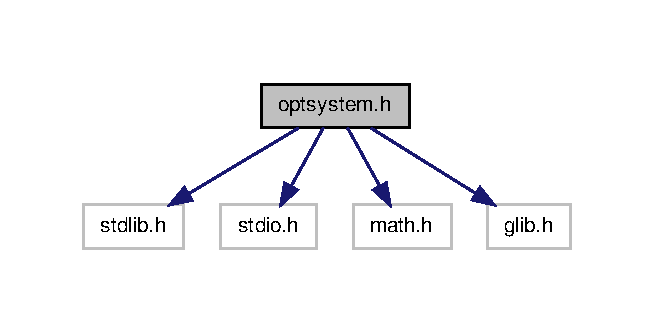
\includegraphics[width=314pt]{d5/d16/a00029}
\end{center}
\end{figure}
\-This graph shows which files directly or indirectly include this file\-:\nopagebreak
\begin{figure}[H]
\begin{center}
\leavevmode
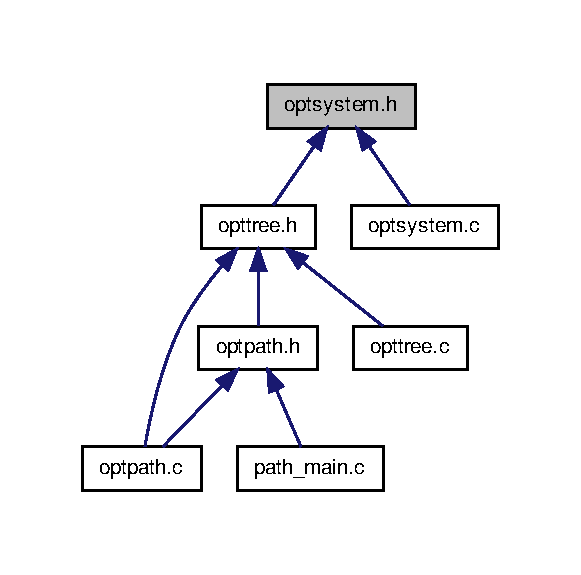
\includegraphics[width=279pt]{d5/d79/a00030}
\end{center}
\end{figure}
\subsection*{\-Data \-Structures}
\begin{DoxyCompactItemize}
\item 
struct \hyperlink{a00006}{\-\_\-region\-\_\-2d\-\_\-t}
\item 
struct \hyperlink{a00007}{\-\_\-state\-\_\-t}
\item 
struct \hyperlink{a00002}{\-\_\-input\-\_\-t}
\item 
struct \hyperlink{a00004}{\-\_\-optsystem\-\_\-t}
\end{DoxyCompactItemize}
\subsection*{\-Defines}
\begin{DoxyCompactItemize}
\item 
\#define \hyperlink{a00018_a6e67a587012cd0570839daca590cf822_a6e67a587012cd0570839daca590cf822}{\-N\-U\-M\-\_\-\-S\-T\-A\-T\-E\-S}~2
\item 
\#define \hyperlink{a00018_ad706a4e66dccbe66985b4c8785f28f3c_ad706a4e66dccbe66985b4c8785f28f3c}{\-N\-U\-M\-\_\-\-I\-N\-P\-U\-T\-S}~1
\end{DoxyCompactItemize}
\subsection*{\-Typedefs}
\begin{DoxyCompactItemize}
\item 
typedef struct \hyperlink{a00006}{\-\_\-region\-\_\-2d\-\_\-t} \hyperlink{a00018_a9136102e25aac8406a94d89f5a95bd1f_a9136102e25aac8406a94d89f5a95bd1f}{region\-\_\-2d\-\_\-t}
\item 
typedef struct \hyperlink{a00007}{\-\_\-state\-\_\-t} \hyperlink{a00018_a1c9d0bb39483d4981491e6383b0dbb47_a1c9d0bb39483d4981491e6383b0dbb47}{state\-\_\-t}
\item 
typedef struct \hyperlink{a00002}{\-\_\-input\-\_\-t} \hyperlink{a00018_a8e5c489dcfacb9bd5f2985013638ea12_a8e5c489dcfacb9bd5f2985013638ea12}{input\-\_\-t}
\item 
typedef struct \hyperlink{a00004}{\-\_\-optsystem\-\_\-t} \hyperlink{a00018_a48d08bbb4534f55ba817743a2b91360c_a48d08bbb4534f55ba817743a2b91360c}{optsystem\-\_\-t}
\end{DoxyCompactItemize}
\subsection*{\-Functions}
\begin{DoxyCompactItemize}
\item 
int \hyperlink{a00018_ad37a0c28a54088a6415ad9dd85542379_ad37a0c28a54088a6415ad9dd85542379}{optsystem\-\_\-new\-\_\-system} (\hyperlink{a00018_a48d08bbb4534f55ba817743a2b91360c_a48d08bbb4534f55ba817743a2b91360c}{optsystem\-\_\-t} $\ast$self)
\item 
int \hyperlink{a00018_a1b54dac5618bcfadd941a7585239e52e_a1b54dac5618bcfadd941a7585239e52e}{optsystem\-\_\-free\-\_\-system} (\hyperlink{a00018_a48d08bbb4534f55ba817743a2b91360c_a48d08bbb4534f55ba817743a2b91360c}{optsystem\-\_\-t} $\ast$self)
\item 
\hyperlink{a00018_a1c9d0bb39483d4981491e6383b0dbb47_a1c9d0bb39483d4981491e6383b0dbb47}{state\-\_\-t} $\ast$ \hyperlink{a00018_a7eb5bfb9a16cf6e49245635fa2400465_a7eb5bfb9a16cf6e49245635fa2400465}{optsystem\-\_\-new\-\_\-state} (\hyperlink{a00018_a48d08bbb4534f55ba817743a2b91360c_a48d08bbb4534f55ba817743a2b91360c}{optsystem\-\_\-t} $\ast$self)
\item 
int \hyperlink{a00018_a27f43c59aba7a8c383399066481b18ba_a27f43c59aba7a8c383399066481b18ba}{optsystem\-\_\-free\-\_\-state} (\hyperlink{a00018_a48d08bbb4534f55ba817743a2b91360c_a48d08bbb4534f55ba817743a2b91360c}{optsystem\-\_\-t} $\ast$self, \hyperlink{a00018_a1c9d0bb39483d4981491e6383b0dbb47_a1c9d0bb39483d4981491e6383b0dbb47}{state\-\_\-t} $\ast$state)
\item 
\hyperlink{a00018_a8e5c489dcfacb9bd5f2985013638ea12_a8e5c489dcfacb9bd5f2985013638ea12}{input\-\_\-t} $\ast$ \hyperlink{a00018_ac249533c36b3db8e1236a3ede20c0be2_ac249533c36b3db8e1236a3ede20c0be2}{optsystem\-\_\-new\-\_\-input} (\hyperlink{a00018_a48d08bbb4534f55ba817743a2b91360c_a48d08bbb4534f55ba817743a2b91360c}{optsystem\-\_\-t} $\ast$self)
\item 
int \hyperlink{a00018_aa20115db43f7ad2bc631d4dee3faf439_aa20115db43f7ad2bc631d4dee3faf439}{optsystem\-\_\-free\-\_\-input} (\hyperlink{a00018_a48d08bbb4534f55ba817743a2b91360c_a48d08bbb4534f55ba817743a2b91360c}{optsystem\-\_\-t} $\ast$self, \hyperlink{a00018_a8e5c489dcfacb9bd5f2985013638ea12_a8e5c489dcfacb9bd5f2985013638ea12}{input\-\_\-t} $\ast$input)
\item 
\hyperlink{a00018_a1c9d0bb39483d4981491e6383b0dbb47_a1c9d0bb39483d4981491e6383b0dbb47}{state\-\_\-t} $\ast$ \hyperlink{a00018_adccdea6115438d8427e2969bffd8d87e_adccdea6115438d8427e2969bffd8d87e}{optsystem\-\_\-clone\-\_\-state} (\hyperlink{a00018_a48d08bbb4534f55ba817743a2b91360c_a48d08bbb4534f55ba817743a2b91360c}{optsystem\-\_\-t} $\ast$self, \hyperlink{a00018_a1c9d0bb39483d4981491e6383b0dbb47_a1c9d0bb39483d4981491e6383b0dbb47}{state\-\_\-t} $\ast$state)
\item 
int \hyperlink{a00018_a4b9f82df886ac6634d2ee9532b603163_a4b9f82df886ac6634d2ee9532b603163}{optsystem\-\_\-set\-\_\-initial\-\_\-state} (\hyperlink{a00018_a48d08bbb4534f55ba817743a2b91360c_a48d08bbb4534f55ba817743a2b91360c}{optsystem\-\_\-t} $\ast$self, \hyperlink{a00018_a1c9d0bb39483d4981491e6383b0dbb47_a1c9d0bb39483d4981491e6383b0dbb47}{state\-\_\-t} $\ast$state)
\item 
int \hyperlink{a00018_ad414a4b37c77f9e4324071ee6fc1c1b8_ad414a4b37c77f9e4324071ee6fc1c1b8}{optsystem\-\_\-get\-\_\-initial\-\_\-state} (\hyperlink{a00018_a48d08bbb4534f55ba817743a2b91360c_a48d08bbb4534f55ba817743a2b91360c}{optsystem\-\_\-t} $\ast$self, \hyperlink{a00018_a1c9d0bb39483d4981491e6383b0dbb47_a1c9d0bb39483d4981491e6383b0dbb47}{state\-\_\-t} $\ast$state)
\item 
int \hyperlink{a00018_aa8d351156d5b945f766be43089c406e4_aa8d351156d5b945f766be43089c406e4}{optsystem\-\_\-get\-\_\-num\-\_\-states} (\hyperlink{a00018_a48d08bbb4534f55ba817743a2b91360c_a48d08bbb4534f55ba817743a2b91360c}{optsystem\-\_\-t} $\ast$self)
\item 
double $\ast$ \hyperlink{a00018_a4748b851e592ba16255987990df866dc_a4748b851e592ba16255987990df866dc}{optsystem\-\_\-get\-\_\-state\-\_\-key} (\hyperlink{a00018_a48d08bbb4534f55ba817743a2b91360c_a48d08bbb4534f55ba817743a2b91360c}{optsystem\-\_\-t} $\ast$self, \hyperlink{a00018_a1c9d0bb39483d4981491e6383b0dbb47_a1c9d0bb39483d4981491e6383b0dbb47}{state\-\_\-t} $\ast$state)
\item 
int \hyperlink{a00018_a778500228810cbc69a6d17494f889b87_a778500228810cbc69a6d17494f889b87}{optsystem\-\_\-sample\-\_\-state} (\hyperlink{a00018_a48d08bbb4534f55ba817743a2b91360c_a48d08bbb4534f55ba817743a2b91360c}{optsystem\-\_\-t} $\ast$self, \hyperlink{a00018_a1c9d0bb39483d4981491e6383b0dbb47_a1c9d0bb39483d4981491e6383b0dbb47}{state\-\_\-t} $\ast$random\-\_\-state)
\item 
int \hyperlink{a00018_a2294e6525f29f89ef7c0e3424063df15_a2294e6525f29f89ef7c0e3424063df15}{optsystem\-\_\-sample\-\_\-target\-\_\-state} (\hyperlink{a00018_a48d08bbb4534f55ba817743a2b91360c_a48d08bbb4534f55ba817743a2b91360c}{optsystem\-\_\-t} $\ast$self, \hyperlink{a00018_a1c9d0bb39483d4981491e6383b0dbb47_a1c9d0bb39483d4981491e6383b0dbb47}{state\-\_\-t} $\ast$random\-\_\-state)
\item 
double \hyperlink{a00018_afce48612176b92f14cb7ffcc91259454_afce48612176b92f14cb7ffcc91259454}{optsystem\-\_\-evaluate\-\_\-distance} (\hyperlink{a00018_a48d08bbb4534f55ba817743a2b91360c_a48d08bbb4534f55ba817743a2b91360c}{optsystem\-\_\-t} $\ast$self, \hyperlink{a00018_a1c9d0bb39483d4981491e6383b0dbb47_a1c9d0bb39483d4981491e6383b0dbb47}{state\-\_\-t} $\ast$state\-\_\-from, \hyperlink{a00018_a1c9d0bb39483d4981491e6383b0dbb47_a1c9d0bb39483d4981491e6383b0dbb47}{state\-\_\-t} $\ast$state\-\_\-to)
\item 
double \hyperlink{a00018_acb788463670e5a6ef08d3759e8fc22ba_acb788463670e5a6ef08d3759e8fc22ba}{optsystem\-\_\-evaluate\-\_\-distance\-\_\-for\-\_\-cost} (\hyperlink{a00018_a48d08bbb4534f55ba817743a2b91360c_a48d08bbb4534f55ba817743a2b91360c}{optsystem\-\_\-t} $\ast$self, \-G\-S\-List $\ast$inputs)
\item 
int \hyperlink{a00018_ab7f5b908723750c22585fb8d58f2c17f_ab7f5b908723750c22585fb8d58f2c17f}{optsystem\-\_\-extend\-\_\-to} (\hyperlink{a00018_a48d08bbb4534f55ba817743a2b91360c_a48d08bbb4534f55ba817743a2b91360c}{optsystem\-\_\-t} $\ast$self, \hyperlink{a00018_a1c9d0bb39483d4981491e6383b0dbb47_a1c9d0bb39483d4981491e6383b0dbb47}{state\-\_\-t} $\ast$state\-\_\-from, \hyperlink{a00018_a1c9d0bb39483d4981491e6383b0dbb47_a1c9d0bb39483d4981491e6383b0dbb47}{state\-\_\-t} $\ast$state\-\_\-towards, int $\ast$fully\-\_\-extends, \-G\-S\-List $\ast$$\ast$trajectory, int $\ast$num\-\_\-node\-\_\-states, int $\ast$$\ast$node\-\_\-states, \-G\-S\-List $\ast$$\ast$inputs)
\item 
gboolean \hyperlink{a00018_a6e1675238ed175e198390a142a966fbb_a6e1675238ed175e198390a142a966fbb}{optsystem\-\_\-is\-\_\-reaching\-\_\-target} (\hyperlink{a00018_a48d08bbb4534f55ba817743a2b91360c_a48d08bbb4534f55ba817743a2b91360c}{optsystem\-\_\-t} $\ast$self, \hyperlink{a00018_a1c9d0bb39483d4981491e6383b0dbb47_a1c9d0bb39483d4981491e6383b0dbb47}{state\-\_\-t} $\ast$state)
\item 
gboolean \hyperlink{a00018_a3af82be1a1df5324149ee8a6450e0381_a3af82be1a1df5324149ee8a6450e0381}{optsystem\-\_\-update\-\_\-operating\-\_\-region} (\hyperlink{a00018_a48d08bbb4534f55ba817743a2b91360c_a48d08bbb4534f55ba817743a2b91360c}{optsystem\-\_\-t} $\ast$self, \hyperlink{a00018_a9136102e25aac8406a94d89f5a95bd1f_a9136102e25aac8406a94d89f5a95bd1f}{region\-\_\-2d\-\_\-t} $\ast$operating\-\_\-region)
\item 
gboolean \hyperlink{a00018_a086fb96570b474b5658dc991c8becc79_a086fb96570b474b5658dc991c8becc79}{optsystem\-\_\-update\-\_\-goal\-\_\-region} (\hyperlink{a00018_a48d08bbb4534f55ba817743a2b91360c_a48d08bbb4534f55ba817743a2b91360c}{optsystem\-\_\-t} $\ast$self, \hyperlink{a00018_a9136102e25aac8406a94d89f5a95bd1f_a9136102e25aac8406a94d89f5a95bd1f}{region\-\_\-2d\-\_\-t} $\ast$goal\-\_\-region)
\item 
gboolean \hyperlink{a00018_a0ad4a450490357b767cd191a83d2cdec_a0ad4a450490357b767cd191a83d2cdec}{optsystem\-\_\-update\-\_\-obstacles} (\hyperlink{a00018_a48d08bbb4534f55ba817743a2b91360c_a48d08bbb4534f55ba817743a2b91360c}{optsystem\-\_\-t} $\ast$self, \-G\-S\-List $\ast$obstacle\-\_\-list)
\item 
gboolean \hyperlink{a00018_afaee017543d17527597efd3a34a7c317_afaee017543d17527597efd3a34a7c317}{optsystem\-\_\-update\-\_\-rectangles} (\hyperlink{a00018_a48d08bbb4534f55ba817743a2b91360c_a48d08bbb4534f55ba817743a2b91360c}{optsystem\-\_\-t} $\ast$self, \-G\-S\-List $\ast$rectangle\-\_\-list)
\end{DoxyCompactItemize}


\subsection{\-Define \-Documentation}
\hypertarget{a00018_ad706a4e66dccbe66985b4c8785f28f3c_ad706a4e66dccbe66985b4c8785f28f3c}{\index{optsystem.\-h@{optsystem.\-h}!\-N\-U\-M\-\_\-\-I\-N\-P\-U\-T\-S@{\-N\-U\-M\-\_\-\-I\-N\-P\-U\-T\-S}}
\index{\-N\-U\-M\-\_\-\-I\-N\-P\-U\-T\-S@{\-N\-U\-M\-\_\-\-I\-N\-P\-U\-T\-S}!optsystem.h@{optsystem.\-h}}
\subsubsection[{\-N\-U\-M\-\_\-\-I\-N\-P\-U\-T\-S}]{\setlength{\rightskip}{0pt plus 5cm}\#define {\bf \-N\-U\-M\-\_\-\-I\-N\-P\-U\-T\-S}~1}}\label{d1/d2b/a00018_ad706a4e66dccbe66985b4c8785f28f3c_ad706a4e66dccbe66985b4c8785f28f3c}
\hypertarget{a00018_a6e67a587012cd0570839daca590cf822_a6e67a587012cd0570839daca590cf822}{\index{optsystem.\-h@{optsystem.\-h}!\-N\-U\-M\-\_\-\-S\-T\-A\-T\-E\-S@{\-N\-U\-M\-\_\-\-S\-T\-A\-T\-E\-S}}
\index{\-N\-U\-M\-\_\-\-S\-T\-A\-T\-E\-S@{\-N\-U\-M\-\_\-\-S\-T\-A\-T\-E\-S}!optsystem.h@{optsystem.\-h}}
\subsubsection[{\-N\-U\-M\-\_\-\-S\-T\-A\-T\-E\-S}]{\setlength{\rightskip}{0pt plus 5cm}\#define {\bf \-N\-U\-M\-\_\-\-S\-T\-A\-T\-E\-S}~2}}\label{d1/d2b/a00018_a6e67a587012cd0570839daca590cf822_a6e67a587012cd0570839daca590cf822}


\subsection{\-Typedef \-Documentation}
\hypertarget{a00018_a8e5c489dcfacb9bd5f2985013638ea12_a8e5c489dcfacb9bd5f2985013638ea12}{\index{optsystem.\-h@{optsystem.\-h}!input\-\_\-t@{input\-\_\-t}}
\index{input\-\_\-t@{input\-\_\-t}!optsystem.h@{optsystem.\-h}}
\subsubsection[{input\-\_\-t}]{\setlength{\rightskip}{0pt plus 5cm}typedef struct {\bf \-\_\-input\-\_\-t} {\bf input\-\_\-t}}}\label{d1/d2b/a00018_a8e5c489dcfacb9bd5f2985013638ea12_a8e5c489dcfacb9bd5f2985013638ea12}
\hypertarget{a00018_a48d08bbb4534f55ba817743a2b91360c_a48d08bbb4534f55ba817743a2b91360c}{\index{optsystem.\-h@{optsystem.\-h}!optsystem\-\_\-t@{optsystem\-\_\-t}}
\index{optsystem\-\_\-t@{optsystem\-\_\-t}!optsystem.h@{optsystem.\-h}}
\subsubsection[{optsystem\-\_\-t}]{\setlength{\rightskip}{0pt plus 5cm}typedef struct {\bf \-\_\-optsystem\-\_\-t} {\bf optsystem\-\_\-t}}}\label{d1/d2b/a00018_a48d08bbb4534f55ba817743a2b91360c_a48d08bbb4534f55ba817743a2b91360c}
\hypertarget{a00018_a9136102e25aac8406a94d89f5a95bd1f_a9136102e25aac8406a94d89f5a95bd1f}{\index{optsystem.\-h@{optsystem.\-h}!region\-\_\-2d\-\_\-t@{region\-\_\-2d\-\_\-t}}
\index{region\-\_\-2d\-\_\-t@{region\-\_\-2d\-\_\-t}!optsystem.h@{optsystem.\-h}}
\subsubsection[{region\-\_\-2d\-\_\-t}]{\setlength{\rightskip}{0pt plus 5cm}typedef struct {\bf \-\_\-region\-\_\-2d\-\_\-t} {\bf region\-\_\-2d\-\_\-t}}}\label{d1/d2b/a00018_a9136102e25aac8406a94d89f5a95bd1f_a9136102e25aac8406a94d89f5a95bd1f}
\hypertarget{a00018_a1c9d0bb39483d4981491e6383b0dbb47_a1c9d0bb39483d4981491e6383b0dbb47}{\index{optsystem.\-h@{optsystem.\-h}!state\-\_\-t@{state\-\_\-t}}
\index{state\-\_\-t@{state\-\_\-t}!optsystem.h@{optsystem.\-h}}
\subsubsection[{state\-\_\-t}]{\setlength{\rightskip}{0pt plus 5cm}typedef struct {\bf \-\_\-state\-\_\-t} {\bf state\-\_\-t}}}\label{d1/d2b/a00018_a1c9d0bb39483d4981491e6383b0dbb47_a1c9d0bb39483d4981491e6383b0dbb47}


\subsection{\-Function \-Documentation}
\hypertarget{a00018_adccdea6115438d8427e2969bffd8d87e_adccdea6115438d8427e2969bffd8d87e}{\index{optsystem.\-h@{optsystem.\-h}!optsystem\-\_\-clone\-\_\-state@{optsystem\-\_\-clone\-\_\-state}}
\index{optsystem\-\_\-clone\-\_\-state@{optsystem\-\_\-clone\-\_\-state}!optsystem.h@{optsystem.\-h}}
\subsubsection[{optsystem\-\_\-clone\-\_\-state}]{\setlength{\rightskip}{0pt plus 5cm}{\bf state\-\_\-t}$\ast$ {\bf optsystem\-\_\-clone\-\_\-state} (
\begin{DoxyParamCaption}
\item[{{\bf optsystem\-\_\-t} $\ast$}]{self, }
\item[{{\bf state\-\_\-t} $\ast$}]{state}
\end{DoxyParamCaption}
)}}\label{d1/d2b/a00018_adccdea6115438d8427e2969bffd8d87e_adccdea6115438d8427e2969bffd8d87e}
\hypertarget{a00018_afce48612176b92f14cb7ffcc91259454_afce48612176b92f14cb7ffcc91259454}{\index{optsystem.\-h@{optsystem.\-h}!optsystem\-\_\-evaluate\-\_\-distance@{optsystem\-\_\-evaluate\-\_\-distance}}
\index{optsystem\-\_\-evaluate\-\_\-distance@{optsystem\-\_\-evaluate\-\_\-distance}!optsystem.h@{optsystem.\-h}}
\subsubsection[{optsystem\-\_\-evaluate\-\_\-distance}]{\setlength{\rightskip}{0pt plus 5cm}double {\bf optsystem\-\_\-evaluate\-\_\-distance} (
\begin{DoxyParamCaption}
\item[{{\bf optsystem\-\_\-t} $\ast$}]{self, }
\item[{{\bf state\-\_\-t} $\ast$}]{state\-\_\-from, }
\item[{{\bf state\-\_\-t} $\ast$}]{state\-\_\-to}
\end{DoxyParamCaption}
)}}\label{d1/d2b/a00018_afce48612176b92f14cb7ffcc91259454_afce48612176b92f14cb7ffcc91259454}
\hypertarget{a00018_acb788463670e5a6ef08d3759e8fc22ba_acb788463670e5a6ef08d3759e8fc22ba}{\index{optsystem.\-h@{optsystem.\-h}!optsystem\-\_\-evaluate\-\_\-distance\-\_\-for\-\_\-cost@{optsystem\-\_\-evaluate\-\_\-distance\-\_\-for\-\_\-cost}}
\index{optsystem\-\_\-evaluate\-\_\-distance\-\_\-for\-\_\-cost@{optsystem\-\_\-evaluate\-\_\-distance\-\_\-for\-\_\-cost}!optsystem.h@{optsystem.\-h}}
\subsubsection[{optsystem\-\_\-evaluate\-\_\-distance\-\_\-for\-\_\-cost}]{\setlength{\rightskip}{0pt plus 5cm}double {\bf optsystem\-\_\-evaluate\-\_\-distance\-\_\-for\-\_\-cost} (
\begin{DoxyParamCaption}
\item[{{\bf optsystem\-\_\-t} $\ast$}]{self, }
\item[{\-G\-S\-List $\ast$}]{inputs}
\end{DoxyParamCaption}
)}}\label{d1/d2b/a00018_acb788463670e5a6ef08d3759e8fc22ba_acb788463670e5a6ef08d3759e8fc22ba}
\hypertarget{a00018_ab7f5b908723750c22585fb8d58f2c17f_ab7f5b908723750c22585fb8d58f2c17f}{\index{optsystem.\-h@{optsystem.\-h}!optsystem\-\_\-extend\-\_\-to@{optsystem\-\_\-extend\-\_\-to}}
\index{optsystem\-\_\-extend\-\_\-to@{optsystem\-\_\-extend\-\_\-to}!optsystem.h@{optsystem.\-h}}
\subsubsection[{optsystem\-\_\-extend\-\_\-to}]{\setlength{\rightskip}{0pt plus 5cm}int {\bf optsystem\-\_\-extend\-\_\-to} (
\begin{DoxyParamCaption}
\item[{{\bf optsystem\-\_\-t} $\ast$}]{self, }
\item[{{\bf state\-\_\-t} $\ast$}]{state\-\_\-from, }
\item[{{\bf state\-\_\-t} $\ast$}]{state\-\_\-towards, }
\item[{int $\ast$}]{fully\-\_\-extends, }
\item[{\-G\-S\-List $\ast$$\ast$}]{trajectory, }
\item[{int $\ast$}]{num\-\_\-node\-\_\-states, }
\item[{int $\ast$$\ast$}]{node\-\_\-states, }
\item[{\-G\-S\-List $\ast$$\ast$}]{inputs}
\end{DoxyParamCaption}
)}}\label{d1/d2b/a00018_ab7f5b908723750c22585fb8d58f2c17f_ab7f5b908723750c22585fb8d58f2c17f}
\hypertarget{a00018_aa20115db43f7ad2bc631d4dee3faf439_aa20115db43f7ad2bc631d4dee3faf439}{\index{optsystem.\-h@{optsystem.\-h}!optsystem\-\_\-free\-\_\-input@{optsystem\-\_\-free\-\_\-input}}
\index{optsystem\-\_\-free\-\_\-input@{optsystem\-\_\-free\-\_\-input}!optsystem.h@{optsystem.\-h}}
\subsubsection[{optsystem\-\_\-free\-\_\-input}]{\setlength{\rightskip}{0pt plus 5cm}int {\bf optsystem\-\_\-free\-\_\-input} (
\begin{DoxyParamCaption}
\item[{{\bf optsystem\-\_\-t} $\ast$}]{self, }
\item[{{\bf input\-\_\-t} $\ast$}]{input}
\end{DoxyParamCaption}
)}}\label{d1/d2b/a00018_aa20115db43f7ad2bc631d4dee3faf439_aa20115db43f7ad2bc631d4dee3faf439}
\hypertarget{a00018_a27f43c59aba7a8c383399066481b18ba_a27f43c59aba7a8c383399066481b18ba}{\index{optsystem.\-h@{optsystem.\-h}!optsystem\-\_\-free\-\_\-state@{optsystem\-\_\-free\-\_\-state}}
\index{optsystem\-\_\-free\-\_\-state@{optsystem\-\_\-free\-\_\-state}!optsystem.h@{optsystem.\-h}}
\subsubsection[{optsystem\-\_\-free\-\_\-state}]{\setlength{\rightskip}{0pt plus 5cm}int {\bf optsystem\-\_\-free\-\_\-state} (
\begin{DoxyParamCaption}
\item[{{\bf optsystem\-\_\-t} $\ast$}]{self, }
\item[{{\bf state\-\_\-t} $\ast$}]{state}
\end{DoxyParamCaption}
)}}\label{d1/d2b/a00018_a27f43c59aba7a8c383399066481b18ba_a27f43c59aba7a8c383399066481b18ba}
\hypertarget{a00018_a1b54dac5618bcfadd941a7585239e52e_a1b54dac5618bcfadd941a7585239e52e}{\index{optsystem.\-h@{optsystem.\-h}!optsystem\-\_\-free\-\_\-system@{optsystem\-\_\-free\-\_\-system}}
\index{optsystem\-\_\-free\-\_\-system@{optsystem\-\_\-free\-\_\-system}!optsystem.h@{optsystem.\-h}}
\subsubsection[{optsystem\-\_\-free\-\_\-system}]{\setlength{\rightskip}{0pt plus 5cm}int {\bf optsystem\-\_\-free\-\_\-system} (
\begin{DoxyParamCaption}
\item[{{\bf optsystem\-\_\-t} $\ast$}]{self}
\end{DoxyParamCaption}
)}}\label{d1/d2b/a00018_a1b54dac5618bcfadd941a7585239e52e_a1b54dac5618bcfadd941a7585239e52e}
\hypertarget{a00018_ad414a4b37c77f9e4324071ee6fc1c1b8_ad414a4b37c77f9e4324071ee6fc1c1b8}{\index{optsystem.\-h@{optsystem.\-h}!optsystem\-\_\-get\-\_\-initial\-\_\-state@{optsystem\-\_\-get\-\_\-initial\-\_\-state}}
\index{optsystem\-\_\-get\-\_\-initial\-\_\-state@{optsystem\-\_\-get\-\_\-initial\-\_\-state}!optsystem.h@{optsystem.\-h}}
\subsubsection[{optsystem\-\_\-get\-\_\-initial\-\_\-state}]{\setlength{\rightskip}{0pt plus 5cm}int {\bf optsystem\-\_\-get\-\_\-initial\-\_\-state} (
\begin{DoxyParamCaption}
\item[{{\bf optsystem\-\_\-t} $\ast$}]{self, }
\item[{{\bf state\-\_\-t} $\ast$}]{state}
\end{DoxyParamCaption}
)}}\label{d1/d2b/a00018_ad414a4b37c77f9e4324071ee6fc1c1b8_ad414a4b37c77f9e4324071ee6fc1c1b8}
\hypertarget{a00018_aa8d351156d5b945f766be43089c406e4_aa8d351156d5b945f766be43089c406e4}{\index{optsystem.\-h@{optsystem.\-h}!optsystem\-\_\-get\-\_\-num\-\_\-states@{optsystem\-\_\-get\-\_\-num\-\_\-states}}
\index{optsystem\-\_\-get\-\_\-num\-\_\-states@{optsystem\-\_\-get\-\_\-num\-\_\-states}!optsystem.h@{optsystem.\-h}}
\subsubsection[{optsystem\-\_\-get\-\_\-num\-\_\-states}]{\setlength{\rightskip}{0pt plus 5cm}int {\bf optsystem\-\_\-get\-\_\-num\-\_\-states} (
\begin{DoxyParamCaption}
\item[{{\bf optsystem\-\_\-t} $\ast$}]{self}
\end{DoxyParamCaption}
)}}\label{d1/d2b/a00018_aa8d351156d5b945f766be43089c406e4_aa8d351156d5b945f766be43089c406e4}
\hypertarget{a00018_a4748b851e592ba16255987990df866dc_a4748b851e592ba16255987990df866dc}{\index{optsystem.\-h@{optsystem.\-h}!optsystem\-\_\-get\-\_\-state\-\_\-key@{optsystem\-\_\-get\-\_\-state\-\_\-key}}
\index{optsystem\-\_\-get\-\_\-state\-\_\-key@{optsystem\-\_\-get\-\_\-state\-\_\-key}!optsystem.h@{optsystem.\-h}}
\subsubsection[{optsystem\-\_\-get\-\_\-state\-\_\-key}]{\setlength{\rightskip}{0pt plus 5cm}double$\ast$ {\bf optsystem\-\_\-get\-\_\-state\-\_\-key} (
\begin{DoxyParamCaption}
\item[{{\bf optsystem\-\_\-t} $\ast$}]{self, }
\item[{{\bf state\-\_\-t} $\ast$}]{state}
\end{DoxyParamCaption}
)}}\label{d1/d2b/a00018_a4748b851e592ba16255987990df866dc_a4748b851e592ba16255987990df866dc}
\hypertarget{a00018_a6e1675238ed175e198390a142a966fbb_a6e1675238ed175e198390a142a966fbb}{\index{optsystem.\-h@{optsystem.\-h}!optsystem\-\_\-is\-\_\-reaching\-\_\-target@{optsystem\-\_\-is\-\_\-reaching\-\_\-target}}
\index{optsystem\-\_\-is\-\_\-reaching\-\_\-target@{optsystem\-\_\-is\-\_\-reaching\-\_\-target}!optsystem.h@{optsystem.\-h}}
\subsubsection[{optsystem\-\_\-is\-\_\-reaching\-\_\-target}]{\setlength{\rightskip}{0pt plus 5cm}gboolean {\bf optsystem\-\_\-is\-\_\-reaching\-\_\-target} (
\begin{DoxyParamCaption}
\item[{{\bf optsystem\-\_\-t} $\ast$}]{self, }
\item[{{\bf state\-\_\-t} $\ast$}]{state}
\end{DoxyParamCaption}
)}}\label{d1/d2b/a00018_a6e1675238ed175e198390a142a966fbb_a6e1675238ed175e198390a142a966fbb}
\hypertarget{a00018_ac249533c36b3db8e1236a3ede20c0be2_ac249533c36b3db8e1236a3ede20c0be2}{\index{optsystem.\-h@{optsystem.\-h}!optsystem\-\_\-new\-\_\-input@{optsystem\-\_\-new\-\_\-input}}
\index{optsystem\-\_\-new\-\_\-input@{optsystem\-\_\-new\-\_\-input}!optsystem.h@{optsystem.\-h}}
\subsubsection[{optsystem\-\_\-new\-\_\-input}]{\setlength{\rightskip}{0pt plus 5cm}{\bf input\-\_\-t}$\ast$ {\bf optsystem\-\_\-new\-\_\-input} (
\begin{DoxyParamCaption}
\item[{{\bf optsystem\-\_\-t} $\ast$}]{self}
\end{DoxyParamCaption}
)}}\label{d1/d2b/a00018_ac249533c36b3db8e1236a3ede20c0be2_ac249533c36b3db8e1236a3ede20c0be2}
\hypertarget{a00018_a7eb5bfb9a16cf6e49245635fa2400465_a7eb5bfb9a16cf6e49245635fa2400465}{\index{optsystem.\-h@{optsystem.\-h}!optsystem\-\_\-new\-\_\-state@{optsystem\-\_\-new\-\_\-state}}
\index{optsystem\-\_\-new\-\_\-state@{optsystem\-\_\-new\-\_\-state}!optsystem.h@{optsystem.\-h}}
\subsubsection[{optsystem\-\_\-new\-\_\-state}]{\setlength{\rightskip}{0pt plus 5cm}{\bf state\-\_\-t}$\ast$ {\bf optsystem\-\_\-new\-\_\-state} (
\begin{DoxyParamCaption}
\item[{{\bf optsystem\-\_\-t} $\ast$}]{self}
\end{DoxyParamCaption}
)}}\label{d1/d2b/a00018_a7eb5bfb9a16cf6e49245635fa2400465_a7eb5bfb9a16cf6e49245635fa2400465}
\hypertarget{a00018_ad37a0c28a54088a6415ad9dd85542379_ad37a0c28a54088a6415ad9dd85542379}{\index{optsystem.\-h@{optsystem.\-h}!optsystem\-\_\-new\-\_\-system@{optsystem\-\_\-new\-\_\-system}}
\index{optsystem\-\_\-new\-\_\-system@{optsystem\-\_\-new\-\_\-system}!optsystem.h@{optsystem.\-h}}
\subsubsection[{optsystem\-\_\-new\-\_\-system}]{\setlength{\rightskip}{0pt plus 5cm}int {\bf optsystem\-\_\-new\-\_\-system} (
\begin{DoxyParamCaption}
\item[{{\bf optsystem\-\_\-t} $\ast$}]{self}
\end{DoxyParamCaption}
)}}\label{d1/d2b/a00018_ad37a0c28a54088a6415ad9dd85542379_ad37a0c28a54088a6415ad9dd85542379}
\hypertarget{a00018_a778500228810cbc69a6d17494f889b87_a778500228810cbc69a6d17494f889b87}{\index{optsystem.\-h@{optsystem.\-h}!optsystem\-\_\-sample\-\_\-state@{optsystem\-\_\-sample\-\_\-state}}
\index{optsystem\-\_\-sample\-\_\-state@{optsystem\-\_\-sample\-\_\-state}!optsystem.h@{optsystem.\-h}}
\subsubsection[{optsystem\-\_\-sample\-\_\-state}]{\setlength{\rightskip}{0pt plus 5cm}int {\bf optsystem\-\_\-sample\-\_\-state} (
\begin{DoxyParamCaption}
\item[{{\bf optsystem\-\_\-t} $\ast$}]{self, }
\item[{{\bf state\-\_\-t} $\ast$}]{random\-\_\-state}
\end{DoxyParamCaption}
)}}\label{d1/d2b/a00018_a778500228810cbc69a6d17494f889b87_a778500228810cbc69a6d17494f889b87}
\hypertarget{a00018_a2294e6525f29f89ef7c0e3424063df15_a2294e6525f29f89ef7c0e3424063df15}{\index{optsystem.\-h@{optsystem.\-h}!optsystem\-\_\-sample\-\_\-target\-\_\-state@{optsystem\-\_\-sample\-\_\-target\-\_\-state}}
\index{optsystem\-\_\-sample\-\_\-target\-\_\-state@{optsystem\-\_\-sample\-\_\-target\-\_\-state}!optsystem.h@{optsystem.\-h}}
\subsubsection[{optsystem\-\_\-sample\-\_\-target\-\_\-state}]{\setlength{\rightskip}{0pt plus 5cm}int {\bf optsystem\-\_\-sample\-\_\-target\-\_\-state} (
\begin{DoxyParamCaption}
\item[{{\bf optsystem\-\_\-t} $\ast$}]{self, }
\item[{{\bf state\-\_\-t} $\ast$}]{random\-\_\-state}
\end{DoxyParamCaption}
)}}\label{d1/d2b/a00018_a2294e6525f29f89ef7c0e3424063df15_a2294e6525f29f89ef7c0e3424063df15}
\hypertarget{a00018_a4b9f82df886ac6634d2ee9532b603163_a4b9f82df886ac6634d2ee9532b603163}{\index{optsystem.\-h@{optsystem.\-h}!optsystem\-\_\-set\-\_\-initial\-\_\-state@{optsystem\-\_\-set\-\_\-initial\-\_\-state}}
\index{optsystem\-\_\-set\-\_\-initial\-\_\-state@{optsystem\-\_\-set\-\_\-initial\-\_\-state}!optsystem.h@{optsystem.\-h}}
\subsubsection[{optsystem\-\_\-set\-\_\-initial\-\_\-state}]{\setlength{\rightskip}{0pt plus 5cm}int {\bf optsystem\-\_\-set\-\_\-initial\-\_\-state} (
\begin{DoxyParamCaption}
\item[{{\bf optsystem\-\_\-t} $\ast$}]{self, }
\item[{{\bf state\-\_\-t} $\ast$}]{state}
\end{DoxyParamCaption}
)}}\label{d1/d2b/a00018_a4b9f82df886ac6634d2ee9532b603163_a4b9f82df886ac6634d2ee9532b603163}
\hypertarget{a00018_a086fb96570b474b5658dc991c8becc79_a086fb96570b474b5658dc991c8becc79}{\index{optsystem.\-h@{optsystem.\-h}!optsystem\-\_\-update\-\_\-goal\-\_\-region@{optsystem\-\_\-update\-\_\-goal\-\_\-region}}
\index{optsystem\-\_\-update\-\_\-goal\-\_\-region@{optsystem\-\_\-update\-\_\-goal\-\_\-region}!optsystem.h@{optsystem.\-h}}
\subsubsection[{optsystem\-\_\-update\-\_\-goal\-\_\-region}]{\setlength{\rightskip}{0pt plus 5cm}gboolean {\bf optsystem\-\_\-update\-\_\-goal\-\_\-region} (
\begin{DoxyParamCaption}
\item[{{\bf optsystem\-\_\-t} $\ast$}]{self, }
\item[{{\bf region\-\_\-2d\-\_\-t} $\ast$}]{goal\-\_\-region}
\end{DoxyParamCaption}
)}}\label{d1/d2b/a00018_a086fb96570b474b5658dc991c8becc79_a086fb96570b474b5658dc991c8becc79}
\hypertarget{a00018_a0ad4a450490357b767cd191a83d2cdec_a0ad4a450490357b767cd191a83d2cdec}{\index{optsystem.\-h@{optsystem.\-h}!optsystem\-\_\-update\-\_\-obstacles@{optsystem\-\_\-update\-\_\-obstacles}}
\index{optsystem\-\_\-update\-\_\-obstacles@{optsystem\-\_\-update\-\_\-obstacles}!optsystem.h@{optsystem.\-h}}
\subsubsection[{optsystem\-\_\-update\-\_\-obstacles}]{\setlength{\rightskip}{0pt plus 5cm}gboolean {\bf optsystem\-\_\-update\-\_\-obstacles} (
\begin{DoxyParamCaption}
\item[{{\bf optsystem\-\_\-t} $\ast$}]{self, }
\item[{\-G\-S\-List $\ast$}]{obstacle\-\_\-list}
\end{DoxyParamCaption}
)}}\label{d1/d2b/a00018_a0ad4a450490357b767cd191a83d2cdec_a0ad4a450490357b767cd191a83d2cdec}
\hypertarget{a00018_a3af82be1a1df5324149ee8a6450e0381_a3af82be1a1df5324149ee8a6450e0381}{\index{optsystem.\-h@{optsystem.\-h}!optsystem\-\_\-update\-\_\-operating\-\_\-region@{optsystem\-\_\-update\-\_\-operating\-\_\-region}}
\index{optsystem\-\_\-update\-\_\-operating\-\_\-region@{optsystem\-\_\-update\-\_\-operating\-\_\-region}!optsystem.h@{optsystem.\-h}}
\subsubsection[{optsystem\-\_\-update\-\_\-operating\-\_\-region}]{\setlength{\rightskip}{0pt plus 5cm}gboolean {\bf optsystem\-\_\-update\-\_\-operating\-\_\-region} (
\begin{DoxyParamCaption}
\item[{{\bf optsystem\-\_\-t} $\ast$}]{self, }
\item[{{\bf region\-\_\-2d\-\_\-t} $\ast$}]{operating\-\_\-region}
\end{DoxyParamCaption}
)}}\label{d1/d2b/a00018_a3af82be1a1df5324149ee8a6450e0381_a3af82be1a1df5324149ee8a6450e0381}
\hypertarget{a00018_afaee017543d17527597efd3a34a7c317_afaee017543d17527597efd3a34a7c317}{\index{optsystem.\-h@{optsystem.\-h}!optsystem\-\_\-update\-\_\-rectangles@{optsystem\-\_\-update\-\_\-rectangles}}
\index{optsystem\-\_\-update\-\_\-rectangles@{optsystem\-\_\-update\-\_\-rectangles}!optsystem.h@{optsystem.\-h}}
\subsubsection[{optsystem\-\_\-update\-\_\-rectangles}]{\setlength{\rightskip}{0pt plus 5cm}gboolean {\bf optsystem\-\_\-update\-\_\-rectangles} (
\begin{DoxyParamCaption}
\item[{{\bf optsystem\-\_\-t} $\ast$}]{self, }
\item[{\-G\-S\-List $\ast$}]{rectangle\-\_\-list}
\end{DoxyParamCaption}
)}}\label{d1/d2b/a00018_afaee017543d17527597efd3a34a7c317_afaee017543d17527597efd3a34a7c317}

\hypertarget{a00019}{\section{opttree.\-c \-File \-Reference}
\label{dd/da2/a00019}\index{opttree.\-c@{opttree.\-c}}
}
{\ttfamily \#include $<$stdlib.\-h$>$}\*
{\ttfamily \#include $<$stdio.\-h$>$}\*
{\ttfamily \#include $<$math.\-h$>$}\*
{\ttfamily \#include $<$sys/time.\-h$>$}\*
{\ttfamily \#include $<$glib.\-h$>$}\*
{\ttfamily \#include \char`\"{}opttree.\-h\char`\"{}}\*
\-Include dependency graph for opttree.\-c\-:\nopagebreak
\begin{figure}[H]
\begin{center}
\leavevmode
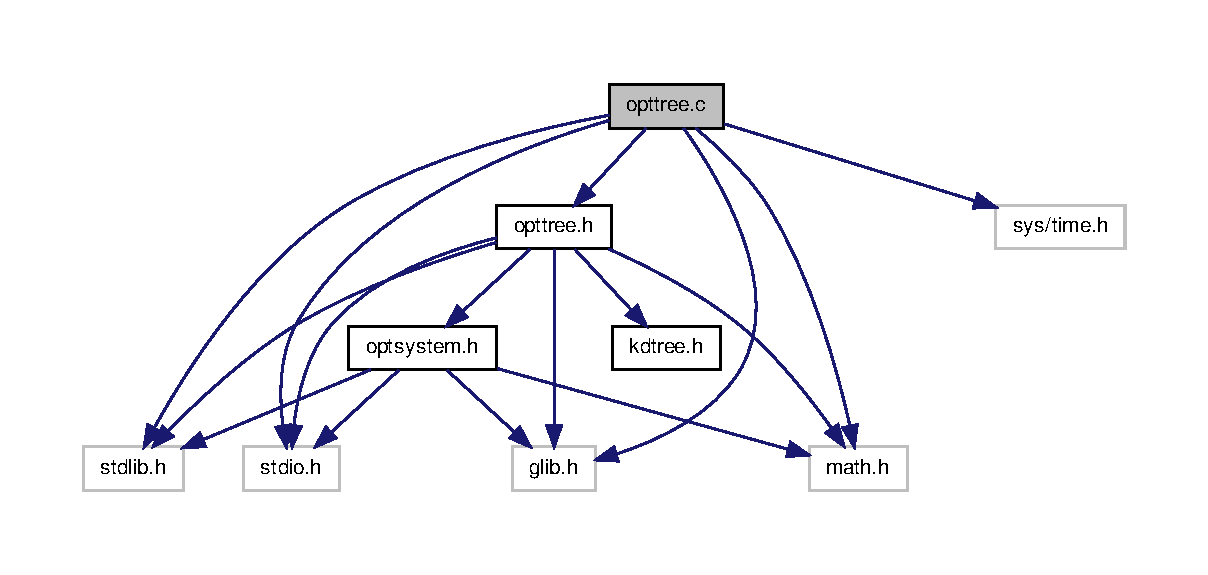
\includegraphics[width=350pt]{df/d61/a00031}
\end{center}
\end{figure}
\subsection*{\-Functions}
\begin{DoxyCompactItemize}
\item 
\hyperlink{a00020_a9c3f304c1ae0687240efd69b7dc98cd6_a9c3f304c1ae0687240efd69b7dc98cd6}{node\-\_\-t} $\ast$ \hyperlink{a00019_a806855fa3cbd142adb06cb12f86af6cf_a806855fa3cbd142adb06cb12f86af6cf}{opttree\-\_\-new\-\_\-node} (\hyperlink{a00020_a07b75293fafb6f31b7e9f723848ad105_a07b75293fafb6f31b7e9f723848ad105}{opttree\-\_\-t} $\ast$self)
\item 
\hyperlink{a00020_a9c3f304c1ae0687240efd69b7dc98cd6_a9c3f304c1ae0687240efd69b7dc98cd6}{node\-\_\-t} $\ast$ \hyperlink{a00019_a7a0fd222dbfa68db41e0cfda4653a0fd_a7a0fd222dbfa68db41e0cfda4653a0fd}{opttree\-\_\-new\-\_\-node\-\_\-no\-\_\-state} ()
\item 
int \hyperlink{a00019_ac3ec357f9dc6bf3500abf3da09a50fdf_ac3ec357f9dc6bf3500abf3da09a50fdf}{opttree\-\_\-free\-\_\-node} (\hyperlink{a00020_a07b75293fafb6f31b7e9f723848ad105_a07b75293fafb6f31b7e9f723848ad105}{opttree\-\_\-t} $\ast$self, \hyperlink{a00020_a9c3f304c1ae0687240efd69b7dc98cd6_a9c3f304c1ae0687240efd69b7dc98cd6}{node\-\_\-t} $\ast$node)
\item 
\hyperlink{a00020_a9c3f304c1ae0687240efd69b7dc98cd6_a9c3f304c1ae0687240efd69b7dc98cd6}{node\-\_\-t} $\ast$ \hyperlink{a00019_ad0c1d9701587dc00f5978ee460b095b9_ad0c1d9701587dc00f5978ee460b095b9}{opttree\-\_\-find\-\_\-nearest\-\_\-neighbor} (\hyperlink{a00020_a07b75293fafb6f31b7e9f723848ad105_a07b75293fafb6f31b7e9f723848ad105}{opttree\-\_\-t} $\ast$self, \hyperlink{a00018_a1c9d0bb39483d4981491e6383b0dbb47_a1c9d0bb39483d4981491e6383b0dbb47}{state\-\_\-t} $\ast$state\-\_\-from)
\item 
void \hyperlink{a00019_a837559b8536b59875d2a4ae3389997b9_a837559b8536b59875d2a4ae3389997b9}{opttree\-\_\-update\-\_\-distance\-\_\-from\-\_\-root} (\hyperlink{a00020_a07b75293fafb6f31b7e9f723848ad105_a07b75293fafb6f31b7e9f723848ad105}{opttree\-\_\-t} $\ast$self, \hyperlink{a00020_a9c3f304c1ae0687240efd69b7dc98cd6_a9c3f304c1ae0687240efd69b7dc98cd6}{node\-\_\-t} $\ast$node\-\_\-parent, \hyperlink{a00020_a9c3f304c1ae0687240efd69b7dc98cd6_a9c3f304c1ae0687240efd69b7dc98cd6}{node\-\_\-t} $\ast$node\-\_\-curr)
\item 
\hyperlink{a00020_a9c3f304c1ae0687240efd69b7dc98cd6_a9c3f304c1ae0687240efd69b7dc98cd6}{node\-\_\-t} $\ast$ \hyperlink{a00019_ac34ccb07ab6ad6b4ea9a46eb2e1d4bc9_ac34ccb07ab6ad6b4ea9a46eb2e1d4bc9}{opttree\-\_\-add\-\_\-traj\-\_\-to\-\_\-graph} (\hyperlink{a00020_a07b75293fafb6f31b7e9f723848ad105_a07b75293fafb6f31b7e9f723848ad105}{opttree\-\_\-t} $\ast$self, \hyperlink{a00020_a9c3f304c1ae0687240efd69b7dc98cd6_a9c3f304c1ae0687240efd69b7dc98cd6}{node\-\_\-t} $\ast$node\-\_\-start, \hyperlink{a00020_a9c3f304c1ae0687240efd69b7dc98cd6_a9c3f304c1ae0687240efd69b7dc98cd6}{node\-\_\-t} $\ast$node\-\_\-end, \-G\-S\-List $\ast$trajectory, int num\-\_\-node\-\_\-states, int $\ast$node\-\_\-states, \-G\-S\-List $\ast$inputs)
\item 
\hyperlink{a00020_a9c3f304c1ae0687240efd69b7dc98cd6_a9c3f304c1ae0687240efd69b7dc98cd6}{node\-\_\-t} $\ast$ \hyperlink{a00019_a4c7ac9f461a2ab5ee216ff5ee1a71581_a4c7ac9f461a2ab5ee216ff5ee1a71581}{opttree\-\_\-extend\-\_\-towards\-\_\-sample} (\hyperlink{a00020_a07b75293fafb6f31b7e9f723848ad105_a07b75293fafb6f31b7e9f723848ad105}{opttree\-\_\-t} $\ast$self, \hyperlink{a00020_a9c3f304c1ae0687240efd69b7dc98cd6_a9c3f304c1ae0687240efd69b7dc98cd6}{node\-\_\-t} $\ast$node\-\_\-from, \hyperlink{a00018_a1c9d0bb39483d4981491e6383b0dbb47_a1c9d0bb39483d4981491e6383b0dbb47}{state\-\_\-t} $\ast$state\-\_\-towards)
\item 
\hyperlink{a00018_a1c9d0bb39483d4981491e6383b0dbb47_a1c9d0bb39483d4981491e6383b0dbb47}{state\-\_\-t} $\ast$ \hyperlink{a00019_a10ca7374cac48feb78ca27aa0f1c5f4b_a10ca7374cac48feb78ca27aa0f1c5f4b}{opttree\-\_\-extend\-\_\-towards\-\_\-sample\-\_\-no\-\_\-create\-\_\-node} (\hyperlink{a00020_a07b75293fafb6f31b7e9f723848ad105_a07b75293fafb6f31b7e9f723848ad105}{opttree\-\_\-t} $\ast$self, \hyperlink{a00020_a9c3f304c1ae0687240efd69b7dc98cd6_a9c3f304c1ae0687240efd69b7dc98cd6}{node\-\_\-t} $\ast$node\-\_\-from, \hyperlink{a00018_a1c9d0bb39483d4981491e6383b0dbb47_a1c9d0bb39483d4981491e6383b0dbb47}{state\-\_\-t} $\ast$state\-\_\-towards)
\item 
\hyperlink{a00020_a9c3f304c1ae0687240efd69b7dc98cd6_a9c3f304c1ae0687240efd69b7dc98cd6}{node\-\_\-t} $\ast$ \hyperlink{a00019_a9b3dc630acdceed59117ab742023e386_a9b3dc630acdceed59117ab742023e386}{opttree\-\_\-find\-\_\-min\-\_\-node\-\_\-in\-\_\-set} (\hyperlink{a00020_a07b75293fafb6f31b7e9f723848ad105_a07b75293fafb6f31b7e9f723848ad105}{opttree\-\_\-t} $\ast$self, \hyperlink{a00018_a1c9d0bb39483d4981491e6383b0dbb47_a1c9d0bb39483d4981491e6383b0dbb47}{state\-\_\-t} $\ast$state\-\_\-towards, \-G\-S\-List $\ast$list\-\_\-nodes)
\item 
\-G\-S\-List $\ast$ \hyperlink{a00019_ad857d6510573bc8771e20d4f290a8cc9_ad857d6510573bc8771e20d4f290a8cc9}{opttree\-\_\-kdtree\-\_\-to\-\_\-gslist} (\hyperlink{a00018_a1c9d0bb39483d4981491e6383b0dbb47_a1c9d0bb39483d4981491e6383b0dbb47}{state\-\_\-t} $\ast$state, \hyperlink{a00020_a7aa4cf85254d52d13693c7328834f6c5_a7aa4cf85254d52d13693c7328834f6c5}{kdres\-\_\-t} $\ast$\hyperlink{a00010}{kdres})
\item 
\-G\-S\-List $\ast$ \hyperlink{a00019_a8713a409c570a5ec10b251b62ee8714e_a8713a409c570a5ec10b251b62ee8714e}{opttree\-\_\-find\-\_\-nodes\-\_\-in\-\_\-ball} (\hyperlink{a00020_a07b75293fafb6f31b7e9f723848ad105_a07b75293fafb6f31b7e9f723848ad105}{opttree\-\_\-t} $\ast$self, \hyperlink{a00018_a1c9d0bb39483d4981491e6383b0dbb47_a1c9d0bb39483d4981491e6383b0dbb47}{state\-\_\-t} $\ast$state, double ball\-\_\-radius)
\item 
int \hyperlink{a00019_a5693c6e43fd9b41afba070ed16bbbcf6_a5693c6e43fd9b41afba070ed16bbbcf6}{opttree\-\_\-extend\-\_\-back\-\_\-to\-\_\-tree} (\hyperlink{a00020_a07b75293fafb6f31b7e9f723848ad105_a07b75293fafb6f31b7e9f723848ad105}{opttree\-\_\-t} $\ast$self, \hyperlink{a00020_a9c3f304c1ae0687240efd69b7dc98cd6_a9c3f304c1ae0687240efd69b7dc98cd6}{node\-\_\-t} $\ast$node\-\_\-from, \-G\-S\-List $\ast$node\-\_\-list)
\item 
int \hyperlink{a00019_a555d69f9356c39303401f79b5e3c02b8_a555d69f9356c39303401f79b5e3c02b8}{opttree\-\_\-iteration} (\hyperlink{a00020_a07b75293fafb6f31b7e9f723848ad105_a07b75293fafb6f31b7e9f723848ad105}{opttree\-\_\-t} $\ast$self)
\item 
int \hyperlink{a00019_a1a94286b5107f470ea340b615cc1e11c_a1a94286b5107f470ea340b615cc1e11c}{opttree\-\_\-reinitialize} (\hyperlink{a00020_a07b75293fafb6f31b7e9f723848ad105_a07b75293fafb6f31b7e9f723848ad105}{opttree\-\_\-t} $\ast$self)
\item 
\hyperlink{a00020_a07b75293fafb6f31b7e9f723848ad105_a07b75293fafb6f31b7e9f723848ad105}{opttree\-\_\-t} $\ast$ \hyperlink{a00019_a9477fb49d51f94d64301104b66f6f193_a9477fb49d51f94d64301104b66f6f193}{opttree\-\_\-create} ()
\item 
int \hyperlink{a00019_a0870ad0ef3b9b2f3ada62a352430f4b1_a0870ad0ef3b9b2f3ada62a352430f4b1}{opttree\-\_\-free\-\_\-tree} (\hyperlink{a00020_a07b75293fafb6f31b7e9f723848ad105_a07b75293fafb6f31b7e9f723848ad105}{opttree\-\_\-t} $\ast$self)
\item 
int \hyperlink{a00019_a87bc01b7917d322ff2ee448bb4055557_a87bc01b7917d322ff2ee448bb4055557}{opttree\-\_\-destroy} (\hyperlink{a00020_a07b75293fafb6f31b7e9f723848ad105_a07b75293fafb6f31b7e9f723848ad105}{opttree\-\_\-t} $\ast$self)
\item 
int \hyperlink{a00019_a7e5472ef1473797978ce8216b345b7fa_a7e5472ef1473797978ce8216b345b7fa}{opttree\-\_\-set\-\_\-root\-\_\-state} (\hyperlink{a00020_a07b75293fafb6f31b7e9f723848ad105_a07b75293fafb6f31b7e9f723848ad105}{opttree\-\_\-t} $\ast$self, \hyperlink{a00018_a1c9d0bb39483d4981491e6383b0dbb47_a1c9d0bb39483d4981491e6383b0dbb47}{state\-\_\-t} $\ast$state)
\end{DoxyCompactItemize}


\subsection{\-Function \-Documentation}
\hypertarget{a00019_ac34ccb07ab6ad6b4ea9a46eb2e1d4bc9_ac34ccb07ab6ad6b4ea9a46eb2e1d4bc9}{\index{opttree.\-c@{opttree.\-c}!opttree\-\_\-add\-\_\-traj\-\_\-to\-\_\-graph@{opttree\-\_\-add\-\_\-traj\-\_\-to\-\_\-graph}}
\index{opttree\-\_\-add\-\_\-traj\-\_\-to\-\_\-graph@{opttree\-\_\-add\-\_\-traj\-\_\-to\-\_\-graph}!opttree.c@{opttree.\-c}}
\subsubsection[{opttree\-\_\-add\-\_\-traj\-\_\-to\-\_\-graph}]{\setlength{\rightskip}{0pt plus 5cm}{\bf node\-\_\-t}$\ast$ {\bf opttree\-\_\-add\-\_\-traj\-\_\-to\-\_\-graph} (
\begin{DoxyParamCaption}
\item[{{\bf opttree\-\_\-t} $\ast$}]{self, }
\item[{{\bf node\-\_\-t} $\ast$}]{node\-\_\-start, }
\item[{{\bf node\-\_\-t} $\ast$}]{node\-\_\-end, }
\item[{\-G\-S\-List $\ast$}]{trajectory, }
\item[{int}]{num\-\_\-node\-\_\-states, }
\item[{int $\ast$}]{node\-\_\-states, }
\item[{\-G\-S\-List $\ast$}]{inputs}
\end{DoxyParamCaption}
)}}\label{dd/da2/a00019_ac34ccb07ab6ad6b4ea9a46eb2e1d4bc9_ac34ccb07ab6ad6b4ea9a46eb2e1d4bc9}
\hypertarget{a00019_a9477fb49d51f94d64301104b66f6f193_a9477fb49d51f94d64301104b66f6f193}{\index{opttree.\-c@{opttree.\-c}!opttree\-\_\-create@{opttree\-\_\-create}}
\index{opttree\-\_\-create@{opttree\-\_\-create}!opttree.c@{opttree.\-c}}
\subsubsection[{opttree\-\_\-create}]{\setlength{\rightskip}{0pt plus 5cm}{\bf opttree\-\_\-t}$\ast$ {\bf opttree\-\_\-create} (
\begin{DoxyParamCaption}
{}
\end{DoxyParamCaption}
)}}\label{dd/da2/a00019_a9477fb49d51f94d64301104b66f6f193_a9477fb49d51f94d64301104b66f6f193}
\hypertarget{a00019_a87bc01b7917d322ff2ee448bb4055557_a87bc01b7917d322ff2ee448bb4055557}{\index{opttree.\-c@{opttree.\-c}!opttree\-\_\-destroy@{opttree\-\_\-destroy}}
\index{opttree\-\_\-destroy@{opttree\-\_\-destroy}!opttree.c@{opttree.\-c}}
\subsubsection[{opttree\-\_\-destroy}]{\setlength{\rightskip}{0pt plus 5cm}int {\bf opttree\-\_\-destroy} (
\begin{DoxyParamCaption}
\item[{{\bf opttree\-\_\-t} $\ast$}]{self}
\end{DoxyParamCaption}
)}}\label{dd/da2/a00019_a87bc01b7917d322ff2ee448bb4055557_a87bc01b7917d322ff2ee448bb4055557}
\hypertarget{a00019_a5693c6e43fd9b41afba070ed16bbbcf6_a5693c6e43fd9b41afba070ed16bbbcf6}{\index{opttree.\-c@{opttree.\-c}!opttree\-\_\-extend\-\_\-back\-\_\-to\-\_\-tree@{opttree\-\_\-extend\-\_\-back\-\_\-to\-\_\-tree}}
\index{opttree\-\_\-extend\-\_\-back\-\_\-to\-\_\-tree@{opttree\-\_\-extend\-\_\-back\-\_\-to\-\_\-tree}!opttree.c@{opttree.\-c}}
\subsubsection[{opttree\-\_\-extend\-\_\-back\-\_\-to\-\_\-tree}]{\setlength{\rightskip}{0pt plus 5cm}int {\bf opttree\-\_\-extend\-\_\-back\-\_\-to\-\_\-tree} (
\begin{DoxyParamCaption}
\item[{{\bf opttree\-\_\-t} $\ast$}]{self, }
\item[{{\bf node\-\_\-t} $\ast$}]{node\-\_\-from, }
\item[{\-G\-S\-List $\ast$}]{node\-\_\-list}
\end{DoxyParamCaption}
)}}\label{dd/da2/a00019_a5693c6e43fd9b41afba070ed16bbbcf6_a5693c6e43fd9b41afba070ed16bbbcf6}
\hypertarget{a00019_a4c7ac9f461a2ab5ee216ff5ee1a71581_a4c7ac9f461a2ab5ee216ff5ee1a71581}{\index{opttree.\-c@{opttree.\-c}!opttree\-\_\-extend\-\_\-towards\-\_\-sample@{opttree\-\_\-extend\-\_\-towards\-\_\-sample}}
\index{opttree\-\_\-extend\-\_\-towards\-\_\-sample@{opttree\-\_\-extend\-\_\-towards\-\_\-sample}!opttree.c@{opttree.\-c}}
\subsubsection[{opttree\-\_\-extend\-\_\-towards\-\_\-sample}]{\setlength{\rightskip}{0pt plus 5cm}{\bf node\-\_\-t}$\ast$ {\bf opttree\-\_\-extend\-\_\-towards\-\_\-sample} (
\begin{DoxyParamCaption}
\item[{{\bf opttree\-\_\-t} $\ast$}]{self, }
\item[{{\bf node\-\_\-t} $\ast$}]{node\-\_\-from, }
\item[{{\bf state\-\_\-t} $\ast$}]{state\-\_\-towards}
\end{DoxyParamCaption}
)}}\label{dd/da2/a00019_a4c7ac9f461a2ab5ee216ff5ee1a71581_a4c7ac9f461a2ab5ee216ff5ee1a71581}
\hypertarget{a00019_a10ca7374cac48feb78ca27aa0f1c5f4b_a10ca7374cac48feb78ca27aa0f1c5f4b}{\index{opttree.\-c@{opttree.\-c}!opttree\-\_\-extend\-\_\-towards\-\_\-sample\-\_\-no\-\_\-create\-\_\-node@{opttree\-\_\-extend\-\_\-towards\-\_\-sample\-\_\-no\-\_\-create\-\_\-node}}
\index{opttree\-\_\-extend\-\_\-towards\-\_\-sample\-\_\-no\-\_\-create\-\_\-node@{opttree\-\_\-extend\-\_\-towards\-\_\-sample\-\_\-no\-\_\-create\-\_\-node}!opttree.c@{opttree.\-c}}
\subsubsection[{opttree\-\_\-extend\-\_\-towards\-\_\-sample\-\_\-no\-\_\-create\-\_\-node}]{\setlength{\rightskip}{0pt plus 5cm}{\bf state\-\_\-t}$\ast$ {\bf opttree\-\_\-extend\-\_\-towards\-\_\-sample\-\_\-no\-\_\-create\-\_\-node} (
\begin{DoxyParamCaption}
\item[{{\bf opttree\-\_\-t} $\ast$}]{self, }
\item[{{\bf node\-\_\-t} $\ast$}]{node\-\_\-from, }
\item[{{\bf state\-\_\-t} $\ast$}]{state\-\_\-towards}
\end{DoxyParamCaption}
)}}\label{dd/da2/a00019_a10ca7374cac48feb78ca27aa0f1c5f4b_a10ca7374cac48feb78ca27aa0f1c5f4b}
\hypertarget{a00019_a9b3dc630acdceed59117ab742023e386_a9b3dc630acdceed59117ab742023e386}{\index{opttree.\-c@{opttree.\-c}!opttree\-\_\-find\-\_\-min\-\_\-node\-\_\-in\-\_\-set@{opttree\-\_\-find\-\_\-min\-\_\-node\-\_\-in\-\_\-set}}
\index{opttree\-\_\-find\-\_\-min\-\_\-node\-\_\-in\-\_\-set@{opttree\-\_\-find\-\_\-min\-\_\-node\-\_\-in\-\_\-set}!opttree.c@{opttree.\-c}}
\subsubsection[{opttree\-\_\-find\-\_\-min\-\_\-node\-\_\-in\-\_\-set}]{\setlength{\rightskip}{0pt plus 5cm}{\bf node\-\_\-t}$\ast$ {\bf opttree\-\_\-find\-\_\-min\-\_\-node\-\_\-in\-\_\-set} (
\begin{DoxyParamCaption}
\item[{{\bf opttree\-\_\-t} $\ast$}]{self, }
\item[{{\bf state\-\_\-t} $\ast$}]{state\-\_\-towards, }
\item[{\-G\-S\-List $\ast$}]{list\-\_\-nodes}
\end{DoxyParamCaption}
)}}\label{dd/da2/a00019_a9b3dc630acdceed59117ab742023e386_a9b3dc630acdceed59117ab742023e386}
\hypertarget{a00019_ad0c1d9701587dc00f5978ee460b095b9_ad0c1d9701587dc00f5978ee460b095b9}{\index{opttree.\-c@{opttree.\-c}!opttree\-\_\-find\-\_\-nearest\-\_\-neighbor@{opttree\-\_\-find\-\_\-nearest\-\_\-neighbor}}
\index{opttree\-\_\-find\-\_\-nearest\-\_\-neighbor@{opttree\-\_\-find\-\_\-nearest\-\_\-neighbor}!opttree.c@{opttree.\-c}}
\subsubsection[{opttree\-\_\-find\-\_\-nearest\-\_\-neighbor}]{\setlength{\rightskip}{0pt plus 5cm}{\bf node\-\_\-t}$\ast$ {\bf opttree\-\_\-find\-\_\-nearest\-\_\-neighbor} (
\begin{DoxyParamCaption}
\item[{{\bf opttree\-\_\-t} $\ast$}]{self, }
\item[{{\bf state\-\_\-t} $\ast$}]{state\-\_\-from}
\end{DoxyParamCaption}
)}}\label{dd/da2/a00019_ad0c1d9701587dc00f5978ee460b095b9_ad0c1d9701587dc00f5978ee460b095b9}
\hypertarget{a00019_a8713a409c570a5ec10b251b62ee8714e_a8713a409c570a5ec10b251b62ee8714e}{\index{opttree.\-c@{opttree.\-c}!opttree\-\_\-find\-\_\-nodes\-\_\-in\-\_\-ball@{opttree\-\_\-find\-\_\-nodes\-\_\-in\-\_\-ball}}
\index{opttree\-\_\-find\-\_\-nodes\-\_\-in\-\_\-ball@{opttree\-\_\-find\-\_\-nodes\-\_\-in\-\_\-ball}!opttree.c@{opttree.\-c}}
\subsubsection[{opttree\-\_\-find\-\_\-nodes\-\_\-in\-\_\-ball}]{\setlength{\rightskip}{0pt plus 5cm}\-G\-S\-List$\ast$ {\bf opttree\-\_\-find\-\_\-nodes\-\_\-in\-\_\-ball} (
\begin{DoxyParamCaption}
\item[{{\bf opttree\-\_\-t} $\ast$}]{self, }
\item[{{\bf state\-\_\-t} $\ast$}]{state, }
\item[{double}]{ball\-\_\-radius}
\end{DoxyParamCaption}
)}}\label{dd/da2/a00019_a8713a409c570a5ec10b251b62ee8714e_a8713a409c570a5ec10b251b62ee8714e}
\hypertarget{a00019_ac3ec357f9dc6bf3500abf3da09a50fdf_ac3ec357f9dc6bf3500abf3da09a50fdf}{\index{opttree.\-c@{opttree.\-c}!opttree\-\_\-free\-\_\-node@{opttree\-\_\-free\-\_\-node}}
\index{opttree\-\_\-free\-\_\-node@{opttree\-\_\-free\-\_\-node}!opttree.c@{opttree.\-c}}
\subsubsection[{opttree\-\_\-free\-\_\-node}]{\setlength{\rightskip}{0pt plus 5cm}int {\bf opttree\-\_\-free\-\_\-node} (
\begin{DoxyParamCaption}
\item[{{\bf opttree\-\_\-t} $\ast$}]{self, }
\item[{{\bf node\-\_\-t} $\ast$}]{node}
\end{DoxyParamCaption}
)}}\label{dd/da2/a00019_ac3ec357f9dc6bf3500abf3da09a50fdf_ac3ec357f9dc6bf3500abf3da09a50fdf}
\hypertarget{a00019_a0870ad0ef3b9b2f3ada62a352430f4b1_a0870ad0ef3b9b2f3ada62a352430f4b1}{\index{opttree.\-c@{opttree.\-c}!opttree\-\_\-free\-\_\-tree@{opttree\-\_\-free\-\_\-tree}}
\index{opttree\-\_\-free\-\_\-tree@{opttree\-\_\-free\-\_\-tree}!opttree.c@{opttree.\-c}}
\subsubsection[{opttree\-\_\-free\-\_\-tree}]{\setlength{\rightskip}{0pt plus 5cm}int {\bf opttree\-\_\-free\-\_\-tree} (
\begin{DoxyParamCaption}
\item[{{\bf opttree\-\_\-t} $\ast$}]{self}
\end{DoxyParamCaption}
)}}\label{dd/da2/a00019_a0870ad0ef3b9b2f3ada62a352430f4b1_a0870ad0ef3b9b2f3ada62a352430f4b1}
\hypertarget{a00019_a555d69f9356c39303401f79b5e3c02b8_a555d69f9356c39303401f79b5e3c02b8}{\index{opttree.\-c@{opttree.\-c}!opttree\-\_\-iteration@{opttree\-\_\-iteration}}
\index{opttree\-\_\-iteration@{opttree\-\_\-iteration}!opttree.c@{opttree.\-c}}
\subsubsection[{opttree\-\_\-iteration}]{\setlength{\rightskip}{0pt plus 5cm}int {\bf opttree\-\_\-iteration} (
\begin{DoxyParamCaption}
\item[{{\bf opttree\-\_\-t} $\ast$}]{self}
\end{DoxyParamCaption}
)}}\label{dd/da2/a00019_a555d69f9356c39303401f79b5e3c02b8_a555d69f9356c39303401f79b5e3c02b8}
\hypertarget{a00019_ad857d6510573bc8771e20d4f290a8cc9_ad857d6510573bc8771e20d4f290a8cc9}{\index{opttree.\-c@{opttree.\-c}!opttree\-\_\-kdtree\-\_\-to\-\_\-gslist@{opttree\-\_\-kdtree\-\_\-to\-\_\-gslist}}
\index{opttree\-\_\-kdtree\-\_\-to\-\_\-gslist@{opttree\-\_\-kdtree\-\_\-to\-\_\-gslist}!opttree.c@{opttree.\-c}}
\subsubsection[{opttree\-\_\-kdtree\-\_\-to\-\_\-gslist}]{\setlength{\rightskip}{0pt plus 5cm}\-G\-S\-List$\ast$ {\bf opttree\-\_\-kdtree\-\_\-to\-\_\-gslist} (
\begin{DoxyParamCaption}
\item[{{\bf state\-\_\-t} $\ast$}]{state, }
\item[{{\bf kdres\-\_\-t} $\ast$}]{kdres}
\end{DoxyParamCaption}
)}}\label{dd/da2/a00019_ad857d6510573bc8771e20d4f290a8cc9_ad857d6510573bc8771e20d4f290a8cc9}
\hypertarget{a00019_a806855fa3cbd142adb06cb12f86af6cf_a806855fa3cbd142adb06cb12f86af6cf}{\index{opttree.\-c@{opttree.\-c}!opttree\-\_\-new\-\_\-node@{opttree\-\_\-new\-\_\-node}}
\index{opttree\-\_\-new\-\_\-node@{opttree\-\_\-new\-\_\-node}!opttree.c@{opttree.\-c}}
\subsubsection[{opttree\-\_\-new\-\_\-node}]{\setlength{\rightskip}{0pt plus 5cm}{\bf node\-\_\-t}$\ast$ {\bf opttree\-\_\-new\-\_\-node} (
\begin{DoxyParamCaption}
\item[{{\bf opttree\-\_\-t} $\ast$}]{self}
\end{DoxyParamCaption}
)}}\label{dd/da2/a00019_a806855fa3cbd142adb06cb12f86af6cf_a806855fa3cbd142adb06cb12f86af6cf}
\hypertarget{a00019_a7a0fd222dbfa68db41e0cfda4653a0fd_a7a0fd222dbfa68db41e0cfda4653a0fd}{\index{opttree.\-c@{opttree.\-c}!opttree\-\_\-new\-\_\-node\-\_\-no\-\_\-state@{opttree\-\_\-new\-\_\-node\-\_\-no\-\_\-state}}
\index{opttree\-\_\-new\-\_\-node\-\_\-no\-\_\-state@{opttree\-\_\-new\-\_\-node\-\_\-no\-\_\-state}!opttree.c@{opttree.\-c}}
\subsubsection[{opttree\-\_\-new\-\_\-node\-\_\-no\-\_\-state}]{\setlength{\rightskip}{0pt plus 5cm}{\bf node\-\_\-t}$\ast$ {\bf opttree\-\_\-new\-\_\-node\-\_\-no\-\_\-state} (
\begin{DoxyParamCaption}
{}
\end{DoxyParamCaption}
)}}\label{dd/da2/a00019_a7a0fd222dbfa68db41e0cfda4653a0fd_a7a0fd222dbfa68db41e0cfda4653a0fd}
\hypertarget{a00019_a1a94286b5107f470ea340b615cc1e11c_a1a94286b5107f470ea340b615cc1e11c}{\index{opttree.\-c@{opttree.\-c}!opttree\-\_\-reinitialize@{opttree\-\_\-reinitialize}}
\index{opttree\-\_\-reinitialize@{opttree\-\_\-reinitialize}!opttree.c@{opttree.\-c}}
\subsubsection[{opttree\-\_\-reinitialize}]{\setlength{\rightskip}{0pt plus 5cm}int {\bf opttree\-\_\-reinitialize} (
\begin{DoxyParamCaption}
\item[{{\bf opttree\-\_\-t} $\ast$}]{self}
\end{DoxyParamCaption}
)}}\label{dd/da2/a00019_a1a94286b5107f470ea340b615cc1e11c_a1a94286b5107f470ea340b615cc1e11c}
\hypertarget{a00019_a7e5472ef1473797978ce8216b345b7fa_a7e5472ef1473797978ce8216b345b7fa}{\index{opttree.\-c@{opttree.\-c}!opttree\-\_\-set\-\_\-root\-\_\-state@{opttree\-\_\-set\-\_\-root\-\_\-state}}
\index{opttree\-\_\-set\-\_\-root\-\_\-state@{opttree\-\_\-set\-\_\-root\-\_\-state}!opttree.c@{opttree.\-c}}
\subsubsection[{opttree\-\_\-set\-\_\-root\-\_\-state}]{\setlength{\rightskip}{0pt plus 5cm}int {\bf opttree\-\_\-set\-\_\-root\-\_\-state} (
\begin{DoxyParamCaption}
\item[{{\bf opttree\-\_\-t} $\ast$}]{self, }
\item[{{\bf state\-\_\-t} $\ast$}]{state}
\end{DoxyParamCaption}
)}}\label{dd/da2/a00019_a7e5472ef1473797978ce8216b345b7fa_a7e5472ef1473797978ce8216b345b7fa}
\hypertarget{a00019_a837559b8536b59875d2a4ae3389997b9_a837559b8536b59875d2a4ae3389997b9}{\index{opttree.\-c@{opttree.\-c}!opttree\-\_\-update\-\_\-distance\-\_\-from\-\_\-root@{opttree\-\_\-update\-\_\-distance\-\_\-from\-\_\-root}}
\index{opttree\-\_\-update\-\_\-distance\-\_\-from\-\_\-root@{opttree\-\_\-update\-\_\-distance\-\_\-from\-\_\-root}!opttree.c@{opttree.\-c}}
\subsubsection[{opttree\-\_\-update\-\_\-distance\-\_\-from\-\_\-root}]{\setlength{\rightskip}{0pt plus 5cm}void {\bf opttree\-\_\-update\-\_\-distance\-\_\-from\-\_\-root} (
\begin{DoxyParamCaption}
\item[{{\bf opttree\-\_\-t} $\ast$}]{self, }
\item[{{\bf node\-\_\-t} $\ast$}]{node\-\_\-parent, }
\item[{{\bf node\-\_\-t} $\ast$}]{node\-\_\-curr}
\end{DoxyParamCaption}
)}}\label{dd/da2/a00019_a837559b8536b59875d2a4ae3389997b9_a837559b8536b59875d2a4ae3389997b9}

\hypertarget{a00020}{\section{opttree.\-h \-File \-Reference}
\label{db/db2/a00020}\index{opttree.\-h@{opttree.\-h}}
}
{\ttfamily \#include $<$stdlib.\-h$>$}\*
{\ttfamily \#include $<$stdio.\-h$>$}\*
{\ttfamily \#include $<$math.\-h$>$}\*
{\ttfamily \#include $<$glib.\-h$>$}\*
{\ttfamily \#include \char`\"{}optsystem.\-h\char`\"{}}\*
{\ttfamily \#include \char`\"{}kdtree.\-h\char`\"{}}\*
\-Include dependency graph for opttree.\-h\-:
\nopagebreak
\begin{figure}[H]
\begin{center}
\leavevmode
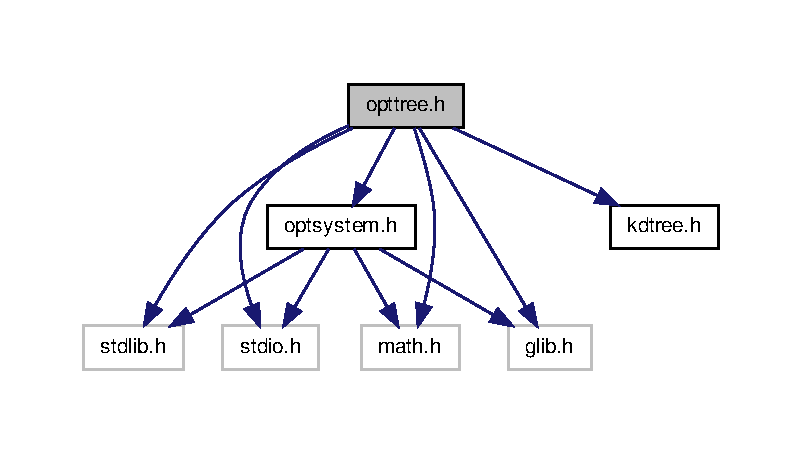
\includegraphics[width=350pt]{dc/d87/a00032}
\end{center}
\end{figure}
\-This graph shows which files directly or indirectly include this file\-:
\nopagebreak
\begin{figure}[H]
\begin{center}
\leavevmode
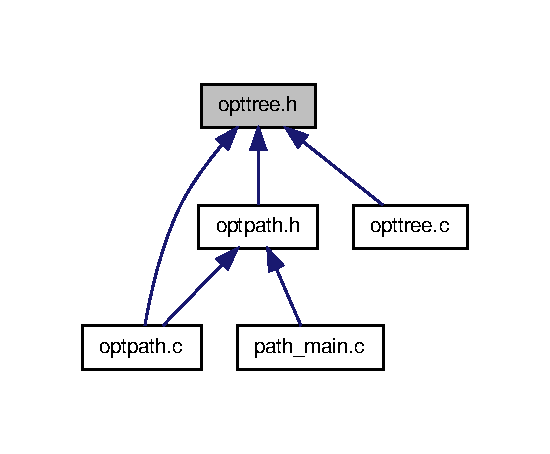
\includegraphics[width=264pt]{d0/dc0/a00033}
\end{center}
\end{figure}
\subsection*{\-Data \-Structures}
\begin{DoxyCompactItemize}
\item 
struct \hyperlink{a00003}{\-\_\-node\-\_\-t}
\item 
struct \hyperlink{a00001}{\-\_\-bounding\-\_\-box\-\_\-t}
\item 
struct \hyperlink{a00005}{\-\_\-opttree\-\_\-t}
\end{DoxyCompactItemize}
\subsection*{\-Typedefs}
\begin{DoxyCompactItemize}
\item 
typedef struct \hyperlink{a00011}{kdtree} \hyperlink{a00020_a3f2e3c0cbfdc70b2db1a09b9aa637a63_a3f2e3c0cbfdc70b2db1a09b9aa637a63}{kdtree\-\_\-t}
\item 
typedef struct \hyperlink{a00010}{kdres} \hyperlink{a00020_a7aa4cf85254d52d13693c7328834f6c5_a7aa4cf85254d52d13693c7328834f6c5}{kdres\-\_\-t}
\item 
typedef struct \hyperlink{a00003}{\-\_\-node\-\_\-t} \hyperlink{a00020_a9c3f304c1ae0687240efd69b7dc98cd6_a9c3f304c1ae0687240efd69b7dc98cd6}{node\-\_\-t}
\item 
typedef struct \hyperlink{a00001}{\-\_\-bounding\-\_\-box\-\_\-t} \hyperlink{a00020_a8cc4dbdff0bcdec2142e75a68b717e6c_a8cc4dbdff0bcdec2142e75a68b717e6c}{bounding\-\_\-box\-\_\-t}
\item 
typedef struct \hyperlink{a00005}{\-\_\-opttree\-\_\-t} \hyperlink{a00020_a07b75293fafb6f31b7e9f723848ad105_a07b75293fafb6f31b7e9f723848ad105}{opttree\-\_\-t}
\end{DoxyCompactItemize}
\subsection*{\-Functions}
\begin{DoxyCompactItemize}
\item 
\hyperlink{a00020_a07b75293fafb6f31b7e9f723848ad105_a07b75293fafb6f31b7e9f723848ad105}{opttree\-\_\-t} $\ast$ \hyperlink{a00020_a9477fb49d51f94d64301104b66f6f193_a9477fb49d51f94d64301104b66f6f193}{opttree\-\_\-create} ()
\item 
int \hyperlink{a00020_a87bc01b7917d322ff2ee448bb4055557_a87bc01b7917d322ff2ee448bb4055557}{opttree\-\_\-destroy} (\hyperlink{a00020_a07b75293fafb6f31b7e9f723848ad105_a07b75293fafb6f31b7e9f723848ad105}{opttree\-\_\-t} $\ast$self)
\item 
int \hyperlink{a00020_a7e5472ef1473797978ce8216b345b7fa_a7e5472ef1473797978ce8216b345b7fa}{opttree\-\_\-set\-\_\-root\-\_\-state} (\hyperlink{a00020_a07b75293fafb6f31b7e9f723848ad105_a07b75293fafb6f31b7e9f723848ad105}{opttree\-\_\-t} $\ast$self, \hyperlink{a00018_a1c9d0bb39483d4981491e6383b0dbb47_a1c9d0bb39483d4981491e6383b0dbb47}{state\-\_\-t} $\ast$state)
\item 
int \hyperlink{a00020_a555d69f9356c39303401f79b5e3c02b8_a555d69f9356c39303401f79b5e3c02b8}{opttree\-\_\-iteration} (\hyperlink{a00020_a07b75293fafb6f31b7e9f723848ad105_a07b75293fafb6f31b7e9f723848ad105}{opttree\-\_\-t} $\ast$self)
\item 
int \hyperlink{a00020_a1a94286b5107f470ea340b615cc1e11c_a1a94286b5107f470ea340b615cc1e11c}{opttree\-\_\-reinitialize} (\hyperlink{a00020_a07b75293fafb6f31b7e9f723848ad105_a07b75293fafb6f31b7e9f723848ad105}{opttree\-\_\-t} $\ast$self)
\end{DoxyCompactItemize}


\subsection{\-Typedef \-Documentation}
\hypertarget{a00020_a8cc4dbdff0bcdec2142e75a68b717e6c_a8cc4dbdff0bcdec2142e75a68b717e6c}{\index{opttree.\-h@{opttree.\-h}!bounding\-\_\-box\-\_\-t@{bounding\-\_\-box\-\_\-t}}
\index{bounding\-\_\-box\-\_\-t@{bounding\-\_\-box\-\_\-t}!opttree.h@{opttree.\-h}}
\subsubsection[{bounding\-\_\-box\-\_\-t}]{\setlength{\rightskip}{0pt plus 5cm}typedef struct {\bf \-\_\-bounding\-\_\-box\-\_\-t}  {\bf bounding\-\_\-box\-\_\-t}}}\label{db/db2/a00020_a8cc4dbdff0bcdec2142e75a68b717e6c_a8cc4dbdff0bcdec2142e75a68b717e6c}
\hypertarget{a00020_a7aa4cf85254d52d13693c7328834f6c5_a7aa4cf85254d52d13693c7328834f6c5}{\index{opttree.\-h@{opttree.\-h}!kdres\-\_\-t@{kdres\-\_\-t}}
\index{kdres\-\_\-t@{kdres\-\_\-t}!opttree.h@{opttree.\-h}}
\subsubsection[{kdres\-\_\-t}]{\setlength{\rightskip}{0pt plus 5cm}typedef struct {\bf kdres} {\bf kdres\-\_\-t}}}\label{db/db2/a00020_a7aa4cf85254d52d13693c7328834f6c5_a7aa4cf85254d52d13693c7328834f6c5}
\hypertarget{a00020_a3f2e3c0cbfdc70b2db1a09b9aa637a63_a3f2e3c0cbfdc70b2db1a09b9aa637a63}{\index{opttree.\-h@{opttree.\-h}!kdtree\-\_\-t@{kdtree\-\_\-t}}
\index{kdtree\-\_\-t@{kdtree\-\_\-t}!opttree.h@{opttree.\-h}}
\subsubsection[{kdtree\-\_\-t}]{\setlength{\rightskip}{0pt plus 5cm}typedef struct {\bf kdtree} {\bf kdtree\-\_\-t}}}\label{db/db2/a00020_a3f2e3c0cbfdc70b2db1a09b9aa637a63_a3f2e3c0cbfdc70b2db1a09b9aa637a63}
\hypertarget{a00020_a9c3f304c1ae0687240efd69b7dc98cd6_a9c3f304c1ae0687240efd69b7dc98cd6}{\index{opttree.\-h@{opttree.\-h}!node\-\_\-t@{node\-\_\-t}}
\index{node\-\_\-t@{node\-\_\-t}!opttree.h@{opttree.\-h}}
\subsubsection[{node\-\_\-t}]{\setlength{\rightskip}{0pt plus 5cm}typedef struct {\bf \-\_\-node\-\_\-t} {\bf node\-\_\-t}}}\label{db/db2/a00020_a9c3f304c1ae0687240efd69b7dc98cd6_a9c3f304c1ae0687240efd69b7dc98cd6}
\hypertarget{a00020_a07b75293fafb6f31b7e9f723848ad105_a07b75293fafb6f31b7e9f723848ad105}{\index{opttree.\-h@{opttree.\-h}!opttree\-\_\-t@{opttree\-\_\-t}}
\index{opttree\-\_\-t@{opttree\-\_\-t}!opttree.h@{opttree.\-h}}
\subsubsection[{opttree\-\_\-t}]{\setlength{\rightskip}{0pt plus 5cm}typedef struct {\bf \-\_\-opttree\-\_\-t} {\bf opttree\-\_\-t}}}\label{db/db2/a00020_a07b75293fafb6f31b7e9f723848ad105_a07b75293fafb6f31b7e9f723848ad105}


\subsection{\-Function \-Documentation}
\hypertarget{a00020_a9477fb49d51f94d64301104b66f6f193_a9477fb49d51f94d64301104b66f6f193}{\index{opttree.\-h@{opttree.\-h}!opttree\-\_\-create@{opttree\-\_\-create}}
\index{opttree\-\_\-create@{opttree\-\_\-create}!opttree.h@{opttree.\-h}}
\subsubsection[{opttree\-\_\-create}]{\setlength{\rightskip}{0pt plus 5cm}{\bf opttree\-\_\-t}$\ast$ {\bf opttree\-\_\-create} (
\begin{DoxyParamCaption}
{}
\end{DoxyParamCaption}
)}}\label{db/db2/a00020_a9477fb49d51f94d64301104b66f6f193_a9477fb49d51f94d64301104b66f6f193}
\hypertarget{a00020_a87bc01b7917d322ff2ee448bb4055557_a87bc01b7917d322ff2ee448bb4055557}{\index{opttree.\-h@{opttree.\-h}!opttree\-\_\-destroy@{opttree\-\_\-destroy}}
\index{opttree\-\_\-destroy@{opttree\-\_\-destroy}!opttree.h@{opttree.\-h}}
\subsubsection[{opttree\-\_\-destroy}]{\setlength{\rightskip}{0pt plus 5cm}int {\bf opttree\-\_\-destroy} (
\begin{DoxyParamCaption}
\item[{{\bf opttree\-\_\-t} $\ast$}]{self}
\end{DoxyParamCaption}
)}}\label{db/db2/a00020_a87bc01b7917d322ff2ee448bb4055557_a87bc01b7917d322ff2ee448bb4055557}
\hypertarget{a00020_a555d69f9356c39303401f79b5e3c02b8_a555d69f9356c39303401f79b5e3c02b8}{\index{opttree.\-h@{opttree.\-h}!opttree\-\_\-iteration@{opttree\-\_\-iteration}}
\index{opttree\-\_\-iteration@{opttree\-\_\-iteration}!opttree.h@{opttree.\-h}}
\subsubsection[{opttree\-\_\-iteration}]{\setlength{\rightskip}{0pt plus 5cm}int {\bf opttree\-\_\-iteration} (
\begin{DoxyParamCaption}
\item[{{\bf opttree\-\_\-t} $\ast$}]{self}
\end{DoxyParamCaption}
)}}\label{db/db2/a00020_a555d69f9356c39303401f79b5e3c02b8_a555d69f9356c39303401f79b5e3c02b8}
\hypertarget{a00020_a1a94286b5107f470ea340b615cc1e11c_a1a94286b5107f470ea340b615cc1e11c}{\index{opttree.\-h@{opttree.\-h}!opttree\-\_\-reinitialize@{opttree\-\_\-reinitialize}}
\index{opttree\-\_\-reinitialize@{opttree\-\_\-reinitialize}!opttree.h@{opttree.\-h}}
\subsubsection[{opttree\-\_\-reinitialize}]{\setlength{\rightskip}{0pt plus 5cm}int {\bf opttree\-\_\-reinitialize} (
\begin{DoxyParamCaption}
\item[{{\bf opttree\-\_\-t} $\ast$}]{self}
\end{DoxyParamCaption}
)}}\label{db/db2/a00020_a1a94286b5107f470ea340b615cc1e11c_a1a94286b5107f470ea340b615cc1e11c}
\hypertarget{a00020_a7e5472ef1473797978ce8216b345b7fa_a7e5472ef1473797978ce8216b345b7fa}{\index{opttree.\-h@{opttree.\-h}!opttree\-\_\-set\-\_\-root\-\_\-state@{opttree\-\_\-set\-\_\-root\-\_\-state}}
\index{opttree\-\_\-set\-\_\-root\-\_\-state@{opttree\-\_\-set\-\_\-root\-\_\-state}!opttree.h@{opttree.\-h}}
\subsubsection[{opttree\-\_\-set\-\_\-root\-\_\-state}]{\setlength{\rightskip}{0pt plus 5cm}int {\bf opttree\-\_\-set\-\_\-root\-\_\-state} (
\begin{DoxyParamCaption}
\item[{{\bf opttree\-\_\-t} $\ast$}]{self, }
\item[{{\bf state\-\_\-t} $\ast$}]{state}
\end{DoxyParamCaption}
)}}\label{db/db2/a00020_a7e5472ef1473797978ce8216b345b7fa_a7e5472ef1473797978ce8216b345b7fa}

\hypertarget{a00021}{\section{path\-\_\-main.\-c \-File \-Reference}
\label{de/d11/a00021}\index{path\-\_\-main.\-c@{path\-\_\-main.\-c}}
}
{\ttfamily \#include \char`\"{}optpath.\-h\char`\"{}}\*
\-Include dependency graph for path\-\_\-main.\-c\-:
\nopagebreak
\begin{figure}[H]
\begin{center}
\leavevmode
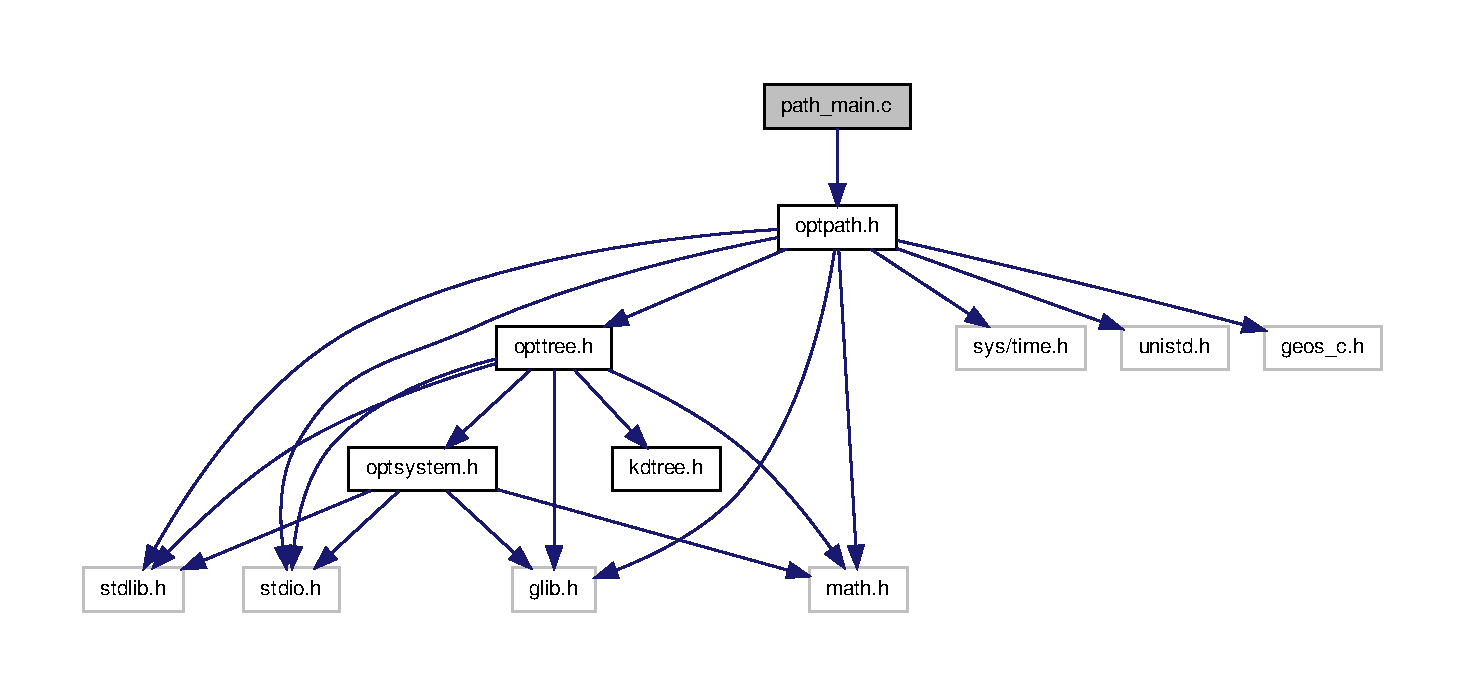
\includegraphics[width=350pt]{db/df3/a00034}
\end{center}
\end{figure}
\subsection*{\-Functions}
\begin{DoxyCompactItemize}
\item 
int \hyperlink{a00021_a0ddf1224851353fc92bfbff6f499fa97_a0ddf1224851353fc92bfbff6f499fa97}{main} (int argc, char $\ast$argv\mbox{[}$\,$\mbox{]})
\begin{DoxyCompactList}\small\item\em program entry \end{DoxyCompactList}\end{DoxyCompactItemize}


\subsection{\-Function \-Documentation}
\hypertarget{a00021_a0ddf1224851353fc92bfbff6f499fa97_a0ddf1224851353fc92bfbff6f499fa97}{\index{path\-\_\-main.\-c@{path\-\_\-main.\-c}!main@{main}}
\index{main@{main}!path_main.c@{path\-\_\-main.\-c}}
\subsubsection[{main}]{\setlength{\rightskip}{0pt plus 5cm}int {\bf main} (
\begin{DoxyParamCaption}
\item[{int}]{argc, }
\item[{char $\ast$}]{argv\mbox{[}$\,$\mbox{]}}
\end{DoxyParamCaption}
)}}\label{de/d11/a00021_a0ddf1224851353fc92bfbff6f499fa97_a0ddf1224851353fc92bfbff6f499fa97}


program entry 


\begin{DoxyParams}{\-Parameters}
{\em argc} & must be 5 to run the program \\
\hline
{\em $\ast$argv\mbox{[}$\,$\mbox{]}} & coordinates of initial point and arrival point \\
\hline
\end{DoxyParams}
\begin{DoxyReturn}{\-Returns}
0 if there were not enough parameter in entry, else 1 
\end{DoxyReturn}

\printindex
\end{document}
